\documentclass[12pt,a4paper]{article}

\usepackage[T1]{fontenc}
\usepackage[utf8]{inputenc}

\usepackage[english]{babel}
\usepackage{csquotes}

\usepackage[authordate-trad,backend=biber]{biblatex-chicago}
\usepackage{acro}
\usepackage{amsmath}
\usepackage{circuitikz}
\usepackage{lmodern}
\usepackage{mathtools}
\usepackage{multirow}
\usepackage{pgf}
\usepackage{todonotes}
\addbibresource{jabref.bib}

\DeclareAcronym{qoe}{
	short=QoE,
	long=Quality of Experience,
}
\DeclareAcronym{qos}{
	short=QoS,
	long=Quality of Service,
}
\DeclareAcronym{p2p}{
	short=P2P,
	long=Peer-to-peer,
}
\DeclareAcronym{cdn}{
	short=CDN,
	long=Content delivery network,
}
\DeclareAcronym{dht}{
short=DHT,
long=Distributed hash-table,
}
\DeclareAcronym{ip}{
	short=IP,
	long=Internet protocol (address),
}
\DeclareAcronym{rtt}{
	short=RTT,
	long=Round-trip time,
}
\DeclareAcronym{tcp}{
short=TCP,
long=Transmission control protocol,
}


\begin{document}

\begin{titlepage}
	\begin{center}
		\vspace*{1cm}
		
		\textbf{By how far have recent churn-reduction techniques improved quality of experience in peer-to-peer video streaming environments?}
		
		\vspace{1.5cm}
		
		\textbf{Martin Symons}
		
		\vfill
		
		A dissertation presented for the degree of\\
		BSc Computer Science
		
		\vspace{0.8cm}
		
		School of Mathematics, Computer Science and Engineering\\
		Liverpool Hope University\\
		United Kingdom\\
		\today
		
	\end{center}
\end{titlepage}

\begin{abstract}
The past decade has proven fruitful for P2P livestreaming research, though limited commercial uptake has kept the total performance improvement vague. To quantify this research, we aim to build three representative models under an \textit{OverSim} simulation and compare in various QoE heuristics. Surveying recent P2P livestreaming research, we find candidate replacements for several modules in popular network \textit{New Coolstreaming}, and select a single competitive monolithic model. In attempting an implementation, we find numerous gaps in \textit{New Coolstreaming}'s literature that negatively impact reproducibility in the research space. A new model, \textit{coolstreaming-spiked}, is proposed to correct these errors without compromising to meet production requirements.  A novel partnership algorithm \textit{Partnerlink} is produced to resolve various unknowns in the \textit{New Coolstreaming} partner relationship program. These algorithms form a more valuable basis for reliable research in the field, whilst remaining compatible with prior \textit{Coolstreaming} research.
\end{abstract}

\section{Declaration of Originality}
I hereby confirm that this assignment is in whole my own work, that no part of it has been copied from any other person's work, published or unpublished, and that any work paraphrased or quoted has been cited and fairly credited in the bibliography.

I have read the guidance provided by Liverpool Hope University and understand the consequences of academic misconduct, including that it may result in the termination of my studies at Liverpool Hope University.

\section{Acknowledgements}
Thanks to my supervisor Mark Greenwood for advising me not only through this paper, but the course as a whole. To everybody else: thanks.

\newpage
\tableofcontents
\listoffigures
\listoftables
\printacronyms[display=all]
\newpage

\section{Introduction} \label{introduction}
Within the past ten years, video streaming traffic across the internet has exploded. Traditional client-server architectures place a large load on the small portion of nodes controlled by the streaming host, and lead to dramatic infrastructure costs. To combat this, peer-to-peer systems have been proposed that spread usage across the network's collective resources. Starting with \textit{DONet/Coolstreaming} in 2004 these networks became defacto for IPTV streaming, their proven utility accelerating research in both pace and complexity. Industry, however, did not take. Since the shutdown of \textit{Coolstreaming} and \textit{PPLive} in the late 2000's, these newer solutions have seen little real-world usage.

As such, the actual impact of current research on network performance is vague. Still, research since has suggested that churn has a substantial and exponential impact on client quality-of-experience (QoE) beyond that which was considered in these original models. This paper attempts to investigate several marked improvements over the best-documented benchmark architecture, \textit{New Coolstreaming}, with particular focus on methods to reduce churn throughout the network. In our proceedings we find several inaccuracies in the specification of this network interrupting our efforts, which we discuss and document. \textit{coolstreaming-spiked} is proposed as an alternative research-oriented model with a strict specification, having these errors corrected. As part of this effort, we produce the novel \textit{Partnerlink} partnership algorithm, forming relationship webs of any scale with minimal link breakage and including a self-healing \textit{panic} mechanism to recover from unexpected failure.

The rest of the paper is structured as follows. Section \ref{litreview} provides a background into P2P livestreaming and defines the research we intended to investigate. This research is compiled into three concrete models in Section \ref{methodology}. Section \ref{implementation} timelines our attempts to produce these models, of which one is completed and tested for effectiveness in Section \ref{results}. Section \ref{problems} explains the problems found in \textit{New Coolstreaming} throughout our implementation attempts. A research-oriented alternative \textit{coolstreaming-spiked} is then formally specified in Section \ref{css}. We conclude in Section \ref{conclusion} and summarize further avenues of research in Section \ref{further}.

\section{Literature Review}  \label{litreview}
We review prior work to understand the essential components of a peer-to-peer livestreaming system, and analyze these piece-by-piece for any potential improvements. These improvements are considered against a generally-understood set of heuristics, providing insight into the QoE for any potential user. We determine our baseline model for comparison, \textit{New Coolstreaming}, and ways in which it could be improved on a modular basis. Finally, we introduce two contemporary monolithic network architectures to represent the state of highly optimized, production-ready designs in current-day research.

Section \ref{litreview:fundamentals} describes the basic analytical model many networks are built from, and its four constituent components. Heuristics used for performance analysis across the P2P video streaming field are established in Section \ref{litreview:heuristics}, alongside a discussion of our focus on churn in Section \ref{litreview:churn}. Components of the prior analytical model are dissected to find potential churn resistance improvements in Sections \ref{litreview:structure}, \ref{litreview:selection} and \ref{litreview:schedulers}, investigating overlay structure, peer selection strategies and chunk schedulers respectively. We introduce \textit{New Coolstreaming} and its older form \textit{DONet} in Section \ref{litreview:coolstreaming}, and pick compatible improvements from our investigations so far in Section \ref{litreview:specifics}. Section \ref{litreview:monoliths} concludes with a discussion on monolithic architectures.

\subsection{Peer-to-Peer Streaming Fundamentals} \label{litreview:fundamentals}
Recent explosions in demand mean video streaming consumes 38\% of current internet traffic (\cite{Sandvine2024}). Despite global innovations in CDN and edge computing technologies, an imbalance still arises in client and server resource availability, forming a bandwidth bottleneck (\cite{Ramzan2012}). Media dissemination at scale hence remains prohibitively expensive. Peer-to-peer protocols aim to spread the bandwidth load across the complete set of peers, detaching bandwidth demands from network size whilst retaining high video quality. These protocols are generally split into VoD and livestreaming purposes, of which we focus on the latter.

Livestreaming presents a unique set of challenges compared to traditional P2P networks like BitTorrent (\cite{Cohen2017}), where QoE is measured mostly by upload speed and piece availability. These two priorities can be trivially arranged through a rarest-first tit-for-tat piece retrieval algorithm; rare pieces are disseminated across the most productive peers to ensure data availability and maximal throughput. Under a livestreaming environment, however, additional constraints apply. Blocks must arrive strictly in-order for efficient filling of client buffers, and end-to-end delay must be minimized to provide a satisfactory "real-time" experience. Different nodes may also maintain different playout positions within the stream, which must be carefully synchronized. Resolution of these factors necessitates network designs unique for this purpose (\cite{Liu2008}).

\cite{Friedman2015} surveys existing designs and expresses their structure in four key modules:

\begin{itemize}
	\item The \textit{player module}, which consumes the received video signal to display to the user. The current playout index and any halting, buffering or chunk skipping mechanisms are also held here.
	\item The \textit{streaming module}, which reads buffered chunks to exchange with neighbors in the overlay, and makes requests on behalf of the player ahead of playout. Depending on the chunk dissemination strategy, discussed in Section \ref{litreview:schedulers}, this will also hold responsibility over gossiping the availability of chunks in the local buffers, or requesting long-term block service through the formation of parent-child relationships.
	\item The \textit{overlay module}, which manages a set of short-term \textit{known} nodes and long-term \textit{neighbor} nodes ready for video transmission. These sets are built mainly from a list retrieved on interval from the origin node or through gossiping.
	\item The \textit{network module}, abstracting the lower-level networking stack and applying any necessary encryption.
\end{itemize}

A node's life therefore begins by spinning up the network module, learning of some nodes to place in its \textit{known} buffer, adapting these to \textit{neighbors} based on some criteria, and exchanging initial block information. Once enough information is gathered, chunks will be requested or transmitted automatically to be stored in memory and eventually played out at the player module. We now explore the metrics used to analyze the performance of this model.

\subsection{Performance Heuristics} \label{litreview:heuristics}
Network heuristics can be broadly classified into two categories: service integrity, covering aspects that apply to any time-series media playback, and audiovisual, describing encoding-specific characteristics in a more subjective manner (\cite{Moltchanov2011}). As our simulation study does not support analysis of the actual encoded signal, we focus for now on the former category.

\cite{Hei2007} describes three key measures in an analysis of the PPLive (\cite{PPLive}) network.
\begin{itemize}
	\item \textit{Playback continuity} (also known as \textit{playout rate} or \textit{playout probability}) is given top priority, measuring the ratio of blocks received by the player module before their playout deadline. 
	\item \textit{Start-up latency} or \textit{start-up delay}, measuring the interval between time of entry to first block playout. This is the first metric impacting user QoE upon network entry, ranking just below continuity in importance.
	\item \textit{Playback delay} or \textit{end-to-end delay}, measuring the interval between a block entering the network until playout at a given node. The importance of this metric depends on the interactivity of a stream: it may rank above start-up delay for real-time purposes, whilst other use cases may prove highly delay-tolerant.
\end{itemize}

These measures correlate various facets of playout quality with user QoE. Additional checks on \textit{bandwidth utilization} and \textit{messaging overhead} can provide insight into the effects of the overlay and streaming modules (\cite{Carta2010}). In our paper, however, we focus on broader aspects of churn and its impact on topology for QoE improvement.

\subsection{Churn} \label{litreview:churn}
In a P2P system, a node's participation is not controlled or supervised; it may leave or join at any time without notification. Particularly under certain overlays, though, the QoE of any node is reliant on that a continued relationship with another - if the partner node leaves, the video stream may suffer an interruption. These dynamics, known on a macro scale as "\textit{churn}," are a fundamental problem that must be solved by any robust P2P system (\cite{Stutzbach2004}).

Churn's impact on QoE is well-studied in structured DHT networks. In this environment, high periods of churn are associated mostly with a hit to startup delay (\cite{Ho2013}). Under the additional constraints of livestreaming, however, this impact expands to cover all measures of performance. \cite{Nanao2012} finds that the mean churn time of a simulation noticably damages forwarding interval and end-to-end delay in topologies where the search time for a new parent is above 100ms. In even the fastest-resolving network discussed in our paper, reselection takes at least three times this interval (\cite{Sina2020}). Simulation analysis in \cite{Kang2012} finds that playout probability across all three tested chunk scheduling strategies also worsens up to 17.2\% under high churn.

Understanding these direct impacts of churn on QoE, we bring particular note to the conclusions of \cite{Vassilakis2010}, drawing correlations from the playout quality and QoE at a node to its chance to churn. Hence, a network with high churn suffers poor QoE, and a network with poor QoE suffers further from worsening churn. This user-driven view of churn is reminiscent of the discovery of the Zipf distribution within P2P file-share peer lifetimes (\cite{Pouwelse2005}), which has since become a research topic in its own right  (\cite{Bustamante}); whether this characterization of P2P streaming churn should be as influential in streaming networks remains an open research question, though its compounding nature leads to its prioritization in our research. Real-world studies on \textit{New Coolstreaming} (discussed in Section \ref{litreview:coolstreaming}) solidify our interest in this area, where churn is described as the most impactful factor on overall performance (\cite{Li2007}).

We now focus on each component of the basic model we have discussed, comparing research under each to find candidate replacements for improved churn management.

\subsection{Overlay Structure} \label{litreview:structure}
Streaming systems can be mostly split into two categories, tree-based and mesh-based. Early P2P streaming networks were designed with the expectation of a rise in IP multicast uptake across the underlying internet, locating multi-host dissemination within the low-level network stack (\cite{Deering1989}). Concerns regarding error correction and scalability eventually prevented this adoption (\cite{Chu2002}), bringing interest to alternative end-to-end approaches.

Designers first moved to single tree overlays, a natural analog to multicast. Tree overlays are structured, with each node forwarding the complete data stream to a greater number of children, administered by a single server at the top of the hierarchy. \cite{Goh2013} finds through comparative simulations that resulting playback delay is up to 114\% lower than in a mesh, observing similar improvements to playout rate. We doubt the validity of these results, however - the paper proposes playback delays shorter than the RTT of a typical single hop in trees of up to 1000 nodes. Still, it is generally understood that tree overlays perform better in delay statistics that than their mesh counterparts \cite{Awiphan2010}, though at the expense of enormous susceptibility to peer churn, since a departing peer temporarily detaches all child nodes from the tree until the overlay heals (\cite{Ghoshal2007}). The uplink bandwidth at each node in a tree also acts as a bottleneck for all children. If any one node cannot transfer the full description as necessary for playout between its children, no alternative source is available for retrieval, and QoS will suffer throughout the remaining tree (\cite{Magharei2007}).

Multi-tree networks have been proposed to mitigate this effect. Video is split into multiple substreams, each directed through an independently managed tree. A peer can join as many trees as necessary to meet playout demand, limited only by its download bandwidth. Since a downstream node retrieves the complete encoding from multiple parents, a single failing node no longer has catastrophic impact on its children. If a layered encoding method is chosen, playout may only degrade in quality instead of buffer (\cite{Zink2004}). Analysis at the time suggested the improved reliability and churn resistance came at the cost of a more complex design and intensive media decoding requirements (\cite{Ghoshal2007}). The former is not a concern for a production network at scale; the latter has since been resolved by the proliferation of advanced hardware video decoding chips and the integration of layered encoding in \textit{de facto} codecs like H.264 (\cite{Seeling2012}). We would now consider that a multi-tree overlay represents a guaranteed improvement over single-tree.

Still, mesh networks have become standard, forming a randomly connected unstructured overlay of parent-child relationships. Each node holds multiple parents and multiple children, resembling a multi-tree; however, nodes can now freely move anywhere in the swarm, using any other node as a source for blocks, without maintaining more than one overlay. Churn recovery is thus bolstered even further, and nodes can easily move away from any detected bottleneck on a given substream (\cite{Magharei2006}). Simulation results in \cite{Magharei2007} suggest bandwidth utilization in mesh networks is universally superior to a tree approach, remaining beyond 90\% of the optimal in all experiments, whilst tree approaches proved less efficient and more sensitive to improperly tuned parameters. At least one additional quality level was received compared to the tree equivalent even when ideally tuned. Bandwidth utilization in a tree is also shown to crater significantly under churn, whilst staying constant in a mesh. We consider these results more reliable than those presented earlier in support of tree networks - Magharei is a respected opinion in overlay construction, being cited within a number of influential papers, and has provided unbiased insight into the field's nuances across their whole portfolio.

In our paper, we consider only mesh networks due to their well-researched performance under a variety of conditions, and their resistance to churn proving relevant to our priorities. That said, hybrid networks combining tree, multi-tree and mesh networks at once have been proposed. A sweeping analysis of these toplogies proves unhelpful due to the wide range of approaches seen in the field. As such, we discuss only the performance of relevant hybrids on a per-network basis later in section \ref{litreview:monoliths}.

\subsection{Peer Selection Strategies} \label{litreview:selection}
Peer selection strategies can be split into three types: random, QoS-aware and locality-aware (\cite{Kim2018}). Random selection methods are highly resilient to churn (\cite{Vishnumurthy2007}) and provide inherent load balancing (\cite{Wang2008}), though at a cost. \textit{PPLive} was noted to suffer very high startup delay of up to 83.5 seconds in some channels, after a failure to quickly accrue quality nodes - the first random batch usually contained nodes with insufficient bandwidth or were unreachable due to network constraints. After 150 seconds, the average node only connected to four parents \cite{Hei2008}. This is not viable compared to today's near-instant CDN delivery; \textit{PPLive}'s popularity proves that this approach can be sufficient, but alternatives should be considered.

QoS-aware methods prioritize nodes by some network heuristic before supply for connection. \textit{OCals} tests RTT both during construction and during scheduling via TCP-Friendly Rate Control (\cite{Floyd2000}), passing as many candidates for which the new node can provide good QoS as those providing good QoS to the node. Compared to established random selection strategy \textit{SCAMP}, startup delay remains approximately constant whilst average throughput increases 103\% in a 1000 node network. Gossiped heuristics can also provide system benefit. Nodes under \textit{Chameleon} (\cite{Nguyen2010}) are bootstrapped with random nodes by \textit{SCAMP}; the overlay then moves nodes matching a heuristic against the requested \textit{quality level} closer together. Senders within these nodes are filtered again based on matching upload/download bandwidth and lowest available layer count. This strategy massively improves playout probability at scale whilst boosting quality satisfaction up to 24.7\% in smaller networks, when compared to simpler bandwidth-based mechanism \textit{FABALAM} (\cite{Liu2004}).

Locality-aware methods are the black sheep of the family, primarily aiding underlay efficiency instead of overlay performance. They reduce end-to-end delays to a minimum, though lack the churn-resilience and throughput utilization better provided by QoS or even random approaches (\cite{Zhao2012}). Fluid representations of the selection strategy categories proved that locality-aware methods can push better performance in networks with universally high RTT (\cite{CoutodaSilva2011}), though this is a rarity in today's highly capable networks. \cite{Magharei2014} proposes \textit{OLIVE}, explicitly aiming to reduce demand on the underlying routing hardware and support the best-effort internet. Though this is a valiant effort, compromises to playout quality for the sake of such optimizations are unlikely to see uptake until a minimum QoS barrier is crossed.

Improvements originating in selection strategy can be amplified by exercising the strategy  wherever possible across the network. \cite{Budhkar2017} proposes three unique sorting algorithms across the network. At entry, the origin node prioritizes peers with high upload bandwidth and a full buffer. Entering nodes filter this list further according to locally perceived upload, propagation delay, lag and buffer before initiating connections. Throughout a node's lifetime, the overlay module scores all ancestors once more to slowly drive performance as playout continues. This thorough application of principles reduces startup delay by 10\% in all cases, and playback delay and parent search time by up to 20\% under churn. This may incur additional performance costs local to each node - however, modern hardware should be capable of these calculations without meaningful strain.

\subsection{Chunk Schedulers} \label{litreview:schedulers}
Chunk schedulers under a mesh topology are generally split into pull, push and hybrid-push-pull approaches, depending on the node taking responsibility of chunk selection. Whilst most aspects of P2P live streaming have been thoroughly surveyed, insights into the ideal scheduler approach appear limited to suppositions made in the proposal of new overlays, and a complete survey remains an open research question.

Pull schemes run the scheduler on the child node, whom determines blocks to request from its parents based on the status of their buffer maps. Overhead under this scheme is high: the sequential processes of neighbor selection, buffer map exchange, chunk selection, request and finally delivery add up, resulting in high end-to-end delay (\cite{Hei2008a}). Such a strategy is therefore rarely proposed for low-latency interactive use (\cite{Zhang2007}). Under mathematical modelling, it is proven that pull schemes provide near-optimal playout probability as long as a node is allowed to push at least three blocks per timestep (\cite{Zhang2014}). Duplication is not an issue, as nodes control exactly when and how each block is received (\cite{LoCigno2008}). Generally speaking, pull schemes are considered "good enough" - even when effort is spent to determine the ideal scheme, \cite{Liang2009} finds through real-world internet experiments that the chunk scheduler only becomes relevant when both the streaming rate approaches maximum throughput for a network and minimal end-to-end delay is desired.

Still, we consider the alternatives. Push schemes have seen some minor uptake. Under this arrangement, the scheduler is run on a parent node automatically pushing received blocks to its children, who attach or leave the parent at will based on their own heuristics. The children, however, have no say in the blocks that they receive; parents instead run an algorithm to determine which block should be pushed to which peer, for which many solutions have been proposed. \cite{Massoulie2007} finds through fluid modelling that the \textit{most deprived peer, random useful chunk} algorithm provides ideal throughput, whilst \cite{Sanghavi2006} theoretically proves the optimal delay of \textit{random peer, latest blind chunk} in pursuit of a hybrid approach. \cite{Bonald2008} notes, however, that the delay performance of the former and throughput of the latter are suboptimal for use in a livestreaming environment. Through simulation and mathematical analysis, the \textit{random peer, latest useful chunk} algorithm is instead found to provide the best compromise between these factors, with methods suggested to reduce message overhead and implementation complexity. Regardless, this does not appear any more optimal than the aforementioned pull schemes, whilst requiring more complex mathematical models to run.

To simplify operations, hybrid-push-pull approaches allow the parent node to push received blocks as before. However, the child nodes are given autonomy to select a subset of blocks to receive, usually by splitting the video into substreams. Such an approach regards the pull mechanism primarily as a routing mechanism, reducing routing, messaging and modelling overhead, whilst maintaining the high bandwidth utilization offered by push networks (\cite{Zhang2007}). The resulting granular control is tempting for those producing monolithic, tightly-optimize overlays, as explored in \ref{litreview:monoliths}.

\subsection{Coolstreaming} \label{litreview:coolstreaming}
We now consider historic implementations of peer-to-peer streaming systems in relation to the above characteristics. An explosion in IPTV popularity in the mid-2000's lead to a great number of new networks - \textit{PPLive}, \textit{SopCast} (\cite{SopCast2019}), \textit{UUSee} (\cite{UUSee2007}) et al. The majority of these networks were commercial endeavors, and therefore closed source.

Of most relevance to our paper is the \textit{Coolstreaming} network. Thanks to its origins in academia, it remained open-source throughout its lifetime despite commercialization, whilst its eventual serving of over 80,000 simultaneous users lead to the gathering of an enormous quantity of data \cite{Li2007}. A great deal of benchmark information is therefore available for our use.

\textit{Coolstreaming} was initially built on the \textit{DONet} architecture, evolving over several years to form the \textit{New Coolstreaming} framework. We provide a brief comparison of both.

\textit{DONet} (\cite{Zhang2005}) forms a mesh-pull topology with random peer selection. Nodes are built of four key components:

\begin{itemize}
	\item The \textit{membership manager}, maintaining a random partial view over the swarm - the \textit{mCache}.
	\item The \textit{partnership manager}, adapting nodes from this view into longer-lived connections suited for video transmission.
	\item The \textit{scheduler}, holding responsibility over the chunk scheduler and requesting blocks from other nodes
	\item The \textit{buffer}, performing playout and acting as a bridge between the overlay and player client.
\end{itemize} 

Each node is provided a unique \textit{NodeID}, usually an IP address. Nodes initially contact a central origin for entry, who redirects to a member chosen at random from its \textit{mCache}. This \textit{deputy node} provides a larger list of random candidates from which the entering node can initiate partnerships and request its first blocks. A membership message is also gossiped as defined under popular protocol \textit{SCAMP} for further \textit{mCache} upkeep.

Nodes begin to exchange buffer maps once partnerships have been established. Partnerships are bidirectional - a node requests and pushes blocks through the same connection. Buffer maps are represented as a single boolean bitmap of length \(B\), where \(B\) is the length of the buffer window. Each entry denotes the availability of one block. Children process these maps through a \textit{rarest-first} chunk scheduling strategy when making requests, giving blocks with only one supplier absolute priority.

Node departure is advertised either by a leaving node itself, or by a partner noticing the departure sending a message on its behalf. On interval, the partnership manager ranks all partners by a score: the average blocks uploaded or average blocks downloaded per unit time, whichever is higher. The worst scoring partner is then swapped out for a fresh member from the \textit{mCache} to converge on better partnerships. A limiting factor \textit{M} is placed on partnership count, provided 4 as example.

In contrast, \textit{New Coolstreaming} (\cite{Li2008}) employs hybrid-push-pull scheduling. This specification poses unique challenges, as explored in Section \ref{implementation}, and so we summarize here with hindsight information. The \textit{SCAMP} protocol has been removed, replaced with a simpler method where the origin node maintains and provides a list of peers directly. Partners from this list are no longer regularly swapped, only \textit{reselected} after any insufficient service is found. Two new heuristics detect this improper service, taking the form of inequalities; one limiting the gap between the local node's buffers and the parent's, and another limiting the gap between the parent's buffers and the rest of the swarm. If these inequalities do not hold, a new partner is swapped in for whom they do.

The buffer and scheduler are coupled to form the \textit{stream manager}. Video is split into substreams, with buffer maps now comprising two tuples - one displaying the most recent block received in each substream, the other a node's subscriptions to the receiving parent. Nodes subscribe to a parent with a single buffer map message, after which the parent will continue to push blocks until the child explicitly unsubscribes or disconnects. The relationship is not broken under any other circumstances.

Finally, a new method for calculating the initial block number is defined, which was not covered as part of \textit{DONet}.

The improvements \textit{New Coolstreaming} proposes against \textit{DONet} are typical of a pull vs hybrid-push-pull mechanism - lower messaging overhead, lower end-to-end delay, and better support for layered video encodings leading to improved QoS. In comparative analysis, median start-up time also reduces from 40 to 24 seconds (\cite{Li2007}). As more data is available on \textit{New Coolstreaming} than \textit{DONet}, and the approach is more in-line with contemporary monoliths, we intend to use \textit{New Coolstreaming} as a benchmark for our analysis. Based on the key components identified above, we now discuss candidate churn-focused improvements that could be suited for \textit{New Coolstreaming}.

\subsection{Coolstreaming-Compatible Churn Improvements} \label{litreview:specifics}
\textit{New Coolstreaming}'s overlay management broadly overlaps with Chameleon's, whose QoS-aware peer selection strategy and resultant churn resistance improvement has already been discussed. \cite{Wang2013} proposes a further measure to adjust a peer's partner count based on its bandwidth, mixing well with \textit{New Coolstreaming}'s existing \textit{M} factor. When taken with the analysis of \cite{Vassilakis2010}, we expect that this should further improve churn resistance - nodes with lesser bandwidth receive worse playout quality on average, and are thus more likely to churn. By subscribing less nodes to these peers, we drive network topology towards longer-lived partnerships. These two papers seem compatible together; we aim to adapt both for \textit{New Coolstreaming}.

\cite{Ho2014} augments \textit{New Coolstreaming}'s chunk scheduler with a complex heuristic involving upload bandwidth, latency and playout delay to determine its downstream quality. Blocks are then sent by priority to nodes which can best service their peers, encouraging lesser nodes to reselect onto them. Simulation experiments within this paper determine its superiority over other simple bandwidth-aware or locality-aware schedulers. Another paper \cite{Li2010} performs more advanced bandwidth \textit{weighting} which may prove competitive, as a substantial reduction in parent reselection rate is shown. However, these results are based on a network with additional functionality, namely a last-effort pull mechanism for missing blocks. Without any means to immediately determine the better approach, we choose to implement the former for its simplicity.

We also propose some improvements outside the traditional view of a P2P architecture. \cite{Wu2009} decouples what a peer uploads from what it views, spreading peer resources to smaller channels to improve their playout quality. Switching delay also improves, and we anticipate that churn chance should also reduce as nodes "stick" to channels for longer, even through disruptive behaviour like channel surfing. Whilst we cannot simulate channel prediction, the inclusion of some ratio of non-playout nodes could provide useful insight. \cite{Huang2010} introduces powerful bootstrap agents into the network, selected for high bandwidth and predicted lifetime, which pre-schedule a download plan for incoming nodes and fill their initial buffer. Churning parents are most disruptive as a node is building its initial buffer for playout, greatly increasing startup delay, so this eliminates a major weak point in \textit{New Coolstreaming}'s current strategy. The existing \textit{DONet} deputy system provides a good baseline for implementation, although the downloading plan cannot be used under \textit{New Coolstreaming} due to the hybrid-push-pull approach. We hope to incorporate both of these novel components into our solution.

We now discuss monolithic solutions developed since the introduction of \textit{New Coolstreaming}. 

\subsection{Monolithic Single Solutions} \label{litreview:monoliths}
\textit{WidePLive} (\cite{Sina2020}) forms a mesh-hybrid-push-pull topology, tightly coupling the overlay construction algorithm with the chunk scheduler via a shared database. Numerous statistics are tracked about each node that are taken into account when finding long-lived, high-contribution peers across both components. A node's actions during the chunk scheduling phase will therefore impact its future position in the overlay, and vice versa. Almost all actions are buffered, prioritized and acted upon after a short period, granting a node greater intelligence about its overlay position and future service. Nodes using the origin as a parent are known as \textit{root peers}, forming a novel load-balancing network to equalize block dissemination between all children. Analysis of these changes against simpler mechanisms similar to those in \textit{PPLive} shows improvement across almost all heuristics: playback latency improves 41.5\%, startup delay improves 67.9\%, and playout rate sees some small improvement. No analysis is performed directly on the impact of churn, however - a gap in literature which we would aim to resolve.

\textit{WidePLive}'s key disadvantage is its complexity. The reference implementation in \textit{OMNeT++} comprises 3000 lines of code. Given the large scope of the project already proposed, an implementation of this network would likely exceed our time constraint.

A promising alternative is seen in the synthesis of two papers. The \textit{AQCS} chunk scheduler (\cite{Guo2008}) marks all blocks in the network as \textit{F} (\textit{forwarding}) or \textit{NF} (\textit{non-forwarding}). All client nodes receiving \textit{F} content will mark it as \textit{NF} and forward it to other peers; any \textit{NF} packets are filtered out on reception. \textit{F} blocks are stored in a buffer. When this buffer becomes empty, the responsible node pulls three new \textit{F} blocks from the origin. If the server completes its backlog of pull requests and becomes idle, it serves one duplicated block to all clients. A last-effort block recovery mechanism is also included. This approach achieves within 10\% of the optimal bandwidth utilization for a P2P system as calculated by a stochastic fluid approach (\cite{Kumar2007}), without the need for any complex scheduling algorithm. This drops to 12\% under churn - an insignificant difference.

\textit{AQCS}'s approach is limited by its need for a fully-connected network, making it unviable for a substantially-sized system. In \cite{Liang2007} a hierarchal overlay construction is therefore discussed, whereby the origin nodes of each \textit{AQCS} cluster form a tree overlay themselves using QoS-aware peer selection. The churn susceptibility of this tree is not a concern due to its small size - in a system with 10 clusters directly owned by the origin, where each cluster holds 20 nodes, the hierarchy can support 4000 peers in two layers. In this way the connection overhead is split across the network, whilst retaining 90\% of optimal bandwidth utilization.

Our results on this system will not fill any gaps in the paper itself, as churn has already been studied. Even so, the logic behind this combined network is much simpler than \textit{WidePLive}, and is more feasible to produce within the time provided. We thus aim to implement this as an additional point of comparison beyond a simple upgrade to \textit{New Coolstreaming}.

This marks the end of our background review. We now summarize the models we have produced, and discuss the means of our analysis.

\section{Methodology} \label{methodology}
Our prior discussion has produced three candidate models:

\begin{itemize}
	\item The default \textit{New Coolstreaming} model, as a baseline.
	\item An enhanced \textit{New Coolstreaming} containing substitute modules proposed in modern research. This includes replacement QoS-aware peer selection strategies and chunk scheduling, decoupling of viewing from uploaded material, and bootstrap nodes to accelerate node entry.
	\item The hierarchical \textit{AQCS} model representing the modern monolithic approach.
\end{itemize}

We aim to produce these three models in a simulation, pitting each in numerous scenarios to gather detailed performance heuristics. Comparisons of this data will reveal the level of improvement at each stage, and any weaknesses of our considered research.

As a simulation environment, we chose \textit{OverSim} (\cite{Baumgart2007}). Its included churn mechanisms, quick-switching between simplified and realistic underlay models, and complete debugging suite eased the otherwise involved development cycle. Ejecting from \textit{OverSim} to \textit{OMNeT++} would also have been trivial, though this was never necessary.

Statistics have been gathered with the built-in \textit{OMNeT++} collection and visualization tools.

\section{Implementation} \label{implementation}
We based our initial experiments on \textit{New Coolstreaming} as described in \cite{Li2008}. We quickly found trouble - whilst the paper describes the stream manager and buffer map exchange in great detail, little space is given to the membership and partnership managers. The upkeep of the \textit{mCache} with incoming peers is unspecified, as is most connection management action related to churning or failing nodes. Some key equations to system function also do not appear. We pushed forward and attempted to fill the blanks ourselves; the final result, whilst technically functional, invariably failed to meet playout across nodes and was in no way correspondent of \textit{New Coolstreaming}'s measured real-world performance.

The \textit{New Coolstreaming} paper concludes its discussion on the problem modules stating \textit{"these basic modules form the base for the initial }Coolstreaming\textit{ system,"} and that \textit{New Coolstreaming} \textit{"has made significant changes in the design of other components."} We thus considered that these modules were holdovers from the older design, implying \textit{New Coolstreaming} must be built up using \textit{DONet/Coolstreaming} as groundwork. We thereby set about an implementation of this more primitive network.

The final \textit{DONet} implementation took two weeks to complete. This network was not fully performant, though the cause was generally understood - as \textit{New Coolstreaming} replaces the buffer, scheduler and related messaging completely, we saw no need to optimize these components. More worryingly, the partnership manager collapsed quickly under even minimal churn. Still, this constituted the groundwork needed to continue.

Returning to the original problem, we found that our architecture still did not align with the basic modules in \textit{New Coolstreaming}. This proved troubling. As discussed later in Section \ref{problems:prodopt}, \textit{DONet} has clarity problems of its own when describing parts of other systems, and we reasoned this might similarly be the case for \textit{New Coolstreaming}. Noticing that the output of these components - \textit{M}-number exchanging partners ready for video transmission - \textit{did} align with the older model, we therefore treated this as a simple faulty description, and moved on to the design of the stream manager.

The well-specified stream manager proved unproblematic, but placed new constraints on the partnership manager that our already brittle implementation could not bear. We hence designed \textit{Partnerlink}, a relationship algorithm reconciling the high-churn overlay with \textit{New Coolstreaming}'s low-churn subscription requirements and performance at scale. This new algorithm integrated well with the wider system, and brought our implementation to a close.

The full development process took over a month. We were therefore not able to complete any further models or make any inter-model comparisons on QoS benefits.

\section{Results and Analysis} \label{results}
We repeat five tests on two scenarios, joining two origin nodes and 30 client nodes over the course of 90 seconds. Nodes live on average 500 seconds before churning; we allow 300 seconds for the overlay to stabilize before a 2000 second measurement period. The 500Kbps source video is split into 10 substreams, containing blocks of one second duration. Partner and membership count \(M\) is limited to 16.

Partner counts are recorded globally as a histogram at each node's playout to gain an overall view of the system. Block statistics are recorded locally as a scalar and averaged across all nodes.

We first test our model on a simple underlay without packet dropping, bandwidth limitations or timeouts. Table \ref{simple_histogram} shows that our partnership mechanism works well in this environment, averaging 15.89 partners across all nodes over the entire measurement period. We also find our manually-tracked potential partner count \(M_c\) to be the same value, though this may not be surprising, as our failure mechanisms are almost never engaged in this abstracted underlay. No node is ever seen below 12 partners in Figure \ref{simple_mc_count}. Our block efficiency shown in Table \ref{simple_scalar} is reasonable - of all received blocks, 3.78\% are duplicates and 2.51\% are outside the bounds of the receiver's buffer, almost all being too old. Despite this, our playout probability is poor: only 64.82\% of blocks are received before playout time, far below expectation.

We test again on a realistic underlay simulating the best-effort internet, including bandwidth limitations, packet loss and queuing. Under this environment, the partnership mechanism fails: despite recording an average \(M_c\) of 13.65 in Table \ref{inet_histogram}, our actual partner count averages 2.04. Figures \ref{inet_mc_count} and \ref{inet_partner_count} reveal a reasonable middle-ground surrounded by nodes simultaneously reporting \(M_c = 16\) and \(partner\ count = 0\) - we explore this and the resultant changes made to \textit{Partnerlink} in section \ref{css:comparison}. Surprisingly, our playout performs very similarly, with a playout rate of 62.66\%. As we believe the partnership manager fails slowly over a node's lifespan, this suggests transmitted blocks must be across relationships made before failure begins; our partnerships are therefore very long lived. This playout rate is in spite of a major hit to efficiency - 9.49\% of all received blocks are now out of bounds, and 8.86\% are now duplicates. The mechanics allowing playout rate to remain so high under these circumstances are unknown.

\begin{table}[h!]
	\centering
	\begin{tabular}{ |p{3cm}||p{3cm}|p{3cm}|p{3cm}|  }
		\hline
		\multicolumn{4}{|c|}{Partner Histograms at Each Simple Playout} \\
		\hline
		Histogram & Mean & Std. & Variance \\
		\hline
		Mc   & 15.89    & 0.33 &   0.11\\
		Partner Count &   15.89  & 0.33   & 0.11\\
		\hline
	\end{tabular} 
	\caption{Statistical analysis of simple underlay partner counts at each playout.}
	\label{simple_histogram}
\end{table}

\begin{table}[h!]
	\centering
	\begin{tabular}{ |p{6cm}||p{3cm}|  }
		\hline
		\multicolumn{2}{|c|}{Block Scalars over Simple Node Lifetime} \\
		\hline
		Scalar & Mean \\
		\hline
		Hit Playouts   & 267.85 \\
		Missed Playouts   & 145.36 \\
		Accepted Blocks   & 273.27 \\
		Out-of-bounds Blocks   & 11.04 \\
		Duplicate Blocks   & 7.34 \\
		\hline
	\end{tabular} 
	\caption{Statistical analysis of simple underlay block statistics throughout the average node's lifetime.}
	\label{simple_scalar}
\end{table}

\begin{table}[h!]
	\centering
	\begin{tabular}{ |p{3cm}||p{3cm}|p{3cm}|p{3cm}|  }
		\hline
		\multicolumn{4}{|c|}{Partner Histograms at Each Inet Playout} \\
		\hline
		Histogram & Mean & Std. & Variance \\
		\hline
		Mc   & 13.65    & 4.24 &   17.98\\
		Partner Count &   2.04  & 3.79  & 14.44 \\
		\hline
	\end{tabular} 
	\caption{Statistical analysis of realistic internet underlay histogram values at each playout.}
	\label{inet_histogram}
\end{table}

\begin{table}[h!]
	\centering
	\begin{tabular}{ |p{6cm}||p{3cm}|  }
		\hline
		\multicolumn{2}{|c|}{Block Scalars over Inet Node Lifetime} \\
		\hline
		Scalar & Mean \\
		\hline
		Hit Playouts   & 171.33 \\
		Missed Playouts   & 102.09 \\
		Accepted Blocks   & 193.53 \\
		Out-of-bounds Blocks   & 18.36 \\
		Duplicate Blocks   & 20.59 \\
		\hline
	\end{tabular} 
	\caption{Statistical analysis of realistic internet underlay block statistics throughout the average node's lifetime.}
	\label{inet_scalar}
\end{table}

\begin{figure}[!ht]
	\centering
	\resizebox{0.7\textwidth}{!}{%
		\input{simple_mc_count.pgf}
	}%
	\caption{Histogram of \(M_c\) at each playout within the simple underlay experiment.}
	\label{simple_mc_count}
\end{figure}

\begin{figure}[!ht]
	\centering
	\resizebox{0.7\textwidth}{!}{%
		%% Creator: Matplotlib, PGF backend
%%
%% To include the figure in your LaTeX document, write
%%   \input{<filename>.pgf}
%%
%% Make sure the required packages are loaded in your preamble
%%   \usepackage{pgf}
%%
%% Also ensure that all the required font packages are loaded; for instance,
%% the lmodern package is sometimes necessary when using math font.
%%   \usepackage{lmodern}
%%
%% Figures using additional raster images can only be included by \input if
%% they are in the same directory as the main LaTeX file. For loading figures
%% from other directories you can use the `import` package
%%   \usepackage{import}
%%
%% and then include the figures with
%%   \import{<path to file>}{<filename>.pgf}
%%
%% Matplotlib used the following preamble
%%   \def\mathdefault#1{#1}
%%   \everymath=\expandafter{\the\everymath\displaystyle}
%%   
%%   \usepackage{fontspec}
%%   \setmainfont{DejaVuSerif.ttf}[Path=\detokenize{/home/sk/.local/lib/python3.10/site-packages/matplotlib/mpl-data/fonts/ttf/}]
%%   \setsansfont{DejaVuSans.ttf}[Path=\detokenize{/home/sk/.local/lib/python3.10/site-packages/matplotlib/mpl-data/fonts/ttf/}]
%%   \setmonofont{DejaVuSansMono.ttf}[Path=\detokenize{/home/sk/.local/lib/python3.10/site-packages/matplotlib/mpl-data/fonts/ttf/}]
%%   \makeatletter\@ifpackageloaded{underscore}{}{\usepackage[strings]{underscore}}\makeatother
%%
\begingroup%
\makeatletter%
\begin{pgfpicture}%
\pgfpathrectangle{\pgfpointorigin}{\pgfqpoint{6.000000in}{4.000000in}}%
\pgfusepath{use as bounding box, clip}%
\begin{pgfscope}%
\pgfsetbuttcap%
\pgfsetmiterjoin%
\definecolor{currentfill}{rgb}{1.000000,1.000000,1.000000}%
\pgfsetfillcolor{currentfill}%
\pgfsetlinewidth{0.000000pt}%
\definecolor{currentstroke}{rgb}{1.000000,1.000000,1.000000}%
\pgfsetstrokecolor{currentstroke}%
\pgfsetdash{}{0pt}%
\pgfpathmoveto{\pgfqpoint{0.000000in}{0.000000in}}%
\pgfpathlineto{\pgfqpoint{6.000000in}{0.000000in}}%
\pgfpathlineto{\pgfqpoint{6.000000in}{4.000000in}}%
\pgfpathlineto{\pgfqpoint{0.000000in}{4.000000in}}%
\pgfpathlineto{\pgfqpoint{0.000000in}{0.000000in}}%
\pgfpathclose%
\pgfusepath{fill}%
\end{pgfscope}%
\begin{pgfscope}%
\pgfsetbuttcap%
\pgfsetmiterjoin%
\definecolor{currentfill}{rgb}{1.000000,1.000000,1.000000}%
\pgfsetfillcolor{currentfill}%
\pgfsetlinewidth{0.000000pt}%
\definecolor{currentstroke}{rgb}{0.000000,0.000000,0.000000}%
\pgfsetstrokecolor{currentstroke}%
\pgfsetstrokeopacity{0.000000}%
\pgfsetdash{}{0pt}%
\pgfpathmoveto{\pgfqpoint{0.905208in}{0.580556in}}%
\pgfpathlineto{\pgfqpoint{5.850000in}{0.580556in}}%
\pgfpathlineto{\pgfqpoint{5.850000in}{3.627778in}}%
\pgfpathlineto{\pgfqpoint{0.905208in}{3.627778in}}%
\pgfpathlineto{\pgfqpoint{0.905208in}{0.580556in}}%
\pgfpathclose%
\pgfusepath{fill}%
\end{pgfscope}%
\begin{pgfscope}%
\pgfpathrectangle{\pgfqpoint{0.905208in}{0.580556in}}{\pgfqpoint{4.944792in}{3.047222in}}%
\pgfusepath{clip}%
\pgfsetbuttcap%
\pgfsetmiterjoin%
\definecolor{currentfill}{rgb}{0.121569,0.466667,0.705882}%
\pgfsetfillcolor{currentfill}%
\pgfsetlinewidth{0.000000pt}%
\definecolor{currentstroke}{rgb}{0.000000,0.000000,0.000000}%
\pgfsetstrokecolor{currentstroke}%
\pgfsetstrokeopacity{0.000000}%
\pgfsetdash{}{0pt}%
\pgfpathmoveto{\pgfqpoint{4.342764in}{0.580556in}}%
\pgfpathlineto{\pgfqpoint{4.342764in}{0.581085in}}%
\pgfpathlineto{\pgfqpoint{4.607191in}{0.581085in}}%
\pgfpathlineto{\pgfqpoint{4.607191in}{0.596160in}}%
\pgfpathlineto{\pgfqpoint{4.871619in}{0.596160in}}%
\pgfpathlineto{\pgfqpoint{4.871619in}{0.805227in}}%
\pgfpathlineto{\pgfqpoint{5.136046in}{0.805227in}}%
\pgfpathlineto{\pgfqpoint{5.136046in}{2.929045in}}%
\pgfpathlineto{\pgfqpoint{5.400473in}{2.929045in}}%
\pgfpathlineto{\pgfqpoint{5.400473in}{0.580556in}}%
\pgfpathlineto{\pgfqpoint{5.136046in}{0.580556in}}%
\pgfpathlineto{\pgfqpoint{5.136046in}{0.580556in}}%
\pgfpathlineto{\pgfqpoint{4.871619in}{0.580556in}}%
\pgfpathlineto{\pgfqpoint{4.871619in}{0.580556in}}%
\pgfpathlineto{\pgfqpoint{4.607191in}{0.580556in}}%
\pgfpathlineto{\pgfqpoint{4.607191in}{0.580556in}}%
\pgfpathlineto{\pgfqpoint{4.342764in}{0.580556in}}%
\pgfpathclose%
\pgfusepath{fill}%
\end{pgfscope}%
\begin{pgfscope}%
\pgfpathrectangle{\pgfqpoint{0.905208in}{0.580556in}}{\pgfqpoint{4.944792in}{3.047222in}}%
\pgfusepath{clip}%
\pgfsetbuttcap%
\pgfsetmiterjoin%
\definecolor{currentfill}{rgb}{1.000000,0.498039,0.054902}%
\pgfsetfillcolor{currentfill}%
\pgfsetlinewidth{0.000000pt}%
\definecolor{currentstroke}{rgb}{0.000000,0.000000,0.000000}%
\pgfsetstrokecolor{currentstroke}%
\pgfsetstrokeopacity{0.000000}%
\pgfsetdash{}{0pt}%
\pgfpathmoveto{\pgfqpoint{4.342764in}{0.580556in}}%
\pgfpathlineto{\pgfqpoint{4.342764in}{0.581393in}}%
\pgfpathlineto{\pgfqpoint{4.607191in}{0.581393in}}%
\pgfpathlineto{\pgfqpoint{4.607191in}{0.599686in}}%
\pgfpathlineto{\pgfqpoint{4.871619in}{0.599686in}}%
\pgfpathlineto{\pgfqpoint{4.871619in}{0.818715in}}%
\pgfpathlineto{\pgfqpoint{5.136046in}{0.818715in}}%
\pgfpathlineto{\pgfqpoint{5.136046in}{3.063398in}}%
\pgfpathlineto{\pgfqpoint{5.400473in}{3.063398in}}%
\pgfpathlineto{\pgfqpoint{5.400473in}{0.580556in}}%
\pgfpathlineto{\pgfqpoint{5.136046in}{0.580556in}}%
\pgfpathlineto{\pgfqpoint{5.136046in}{0.580556in}}%
\pgfpathlineto{\pgfqpoint{4.871619in}{0.580556in}}%
\pgfpathlineto{\pgfqpoint{4.871619in}{0.580556in}}%
\pgfpathlineto{\pgfqpoint{4.607191in}{0.580556in}}%
\pgfpathlineto{\pgfqpoint{4.607191in}{0.580556in}}%
\pgfpathlineto{\pgfqpoint{4.342764in}{0.580556in}}%
\pgfpathclose%
\pgfusepath{fill}%
\end{pgfscope}%
\begin{pgfscope}%
\pgfpathrectangle{\pgfqpoint{0.905208in}{0.580556in}}{\pgfqpoint{4.944792in}{3.047222in}}%
\pgfusepath{clip}%
\pgfsetbuttcap%
\pgfsetmiterjoin%
\definecolor{currentfill}{rgb}{0.172549,0.627451,0.172549}%
\pgfsetfillcolor{currentfill}%
\pgfsetlinewidth{0.000000pt}%
\definecolor{currentstroke}{rgb}{0.000000,0.000000,0.000000}%
\pgfsetstrokecolor{currentstroke}%
\pgfsetstrokeopacity{0.000000}%
\pgfsetdash{}{0pt}%
\pgfpathmoveto{\pgfqpoint{4.342764in}{0.580556in}}%
\pgfpathlineto{\pgfqpoint{4.342764in}{0.581746in}}%
\pgfpathlineto{\pgfqpoint{4.607191in}{0.581746in}}%
\pgfpathlineto{\pgfqpoint{4.607191in}{0.599069in}}%
\pgfpathlineto{\pgfqpoint{4.871619in}{0.599069in}}%
\pgfpathlineto{\pgfqpoint{4.871619in}{0.818759in}}%
\pgfpathlineto{\pgfqpoint{5.136046in}{0.818759in}}%
\pgfpathlineto{\pgfqpoint{5.136046in}{3.119907in}}%
\pgfpathlineto{\pgfqpoint{5.400473in}{3.119907in}}%
\pgfpathlineto{\pgfqpoint{5.400473in}{0.580556in}}%
\pgfpathlineto{\pgfqpoint{5.136046in}{0.580556in}}%
\pgfpathlineto{\pgfqpoint{5.136046in}{0.580556in}}%
\pgfpathlineto{\pgfqpoint{4.871619in}{0.580556in}}%
\pgfpathlineto{\pgfqpoint{4.871619in}{0.580556in}}%
\pgfpathlineto{\pgfqpoint{4.607191in}{0.580556in}}%
\pgfpathlineto{\pgfqpoint{4.607191in}{0.580556in}}%
\pgfpathlineto{\pgfqpoint{4.342764in}{0.580556in}}%
\pgfpathclose%
\pgfusepath{fill}%
\end{pgfscope}%
\begin{pgfscope}%
\pgfpathrectangle{\pgfqpoint{0.905208in}{0.580556in}}{\pgfqpoint{4.944792in}{3.047222in}}%
\pgfusepath{clip}%
\pgfsetbuttcap%
\pgfsetmiterjoin%
\definecolor{currentfill}{rgb}{0.839216,0.152941,0.156863}%
\pgfsetfillcolor{currentfill}%
\pgfsetlinewidth{0.000000pt}%
\definecolor{currentstroke}{rgb}{0.000000,0.000000,0.000000}%
\pgfsetstrokecolor{currentstroke}%
\pgfsetstrokeopacity{0.000000}%
\pgfsetdash{}{0pt}%
\pgfpathmoveto{\pgfqpoint{4.078337in}{0.580556in}}%
\pgfpathlineto{\pgfqpoint{4.078337in}{0.580644in}}%
\pgfpathlineto{\pgfqpoint{4.342764in}{0.580644in}}%
\pgfpathlineto{\pgfqpoint{4.342764in}{0.582010in}}%
\pgfpathlineto{\pgfqpoint{4.607191in}{0.582010in}}%
\pgfpathlineto{\pgfqpoint{4.607191in}{0.602771in}}%
\pgfpathlineto{\pgfqpoint{4.871619in}{0.602771in}}%
\pgfpathlineto{\pgfqpoint{4.871619in}{0.852700in}}%
\pgfpathlineto{\pgfqpoint{5.136046in}{0.852700in}}%
\pgfpathlineto{\pgfqpoint{5.136046in}{2.975857in}}%
\pgfpathlineto{\pgfqpoint{5.400473in}{2.975857in}}%
\pgfpathlineto{\pgfqpoint{5.400473in}{0.580556in}}%
\pgfpathlineto{\pgfqpoint{5.136046in}{0.580556in}}%
\pgfpathlineto{\pgfqpoint{5.136046in}{0.580556in}}%
\pgfpathlineto{\pgfqpoint{4.871619in}{0.580556in}}%
\pgfpathlineto{\pgfqpoint{4.871619in}{0.580556in}}%
\pgfpathlineto{\pgfqpoint{4.607191in}{0.580556in}}%
\pgfpathlineto{\pgfqpoint{4.607191in}{0.580556in}}%
\pgfpathlineto{\pgfqpoint{4.342764in}{0.580556in}}%
\pgfpathlineto{\pgfqpoint{4.342764in}{0.580556in}}%
\pgfpathlineto{\pgfqpoint{4.078337in}{0.580556in}}%
\pgfpathclose%
\pgfusepath{fill}%
\end{pgfscope}%
\begin{pgfscope}%
\pgfpathrectangle{\pgfqpoint{0.905208in}{0.580556in}}{\pgfqpoint{4.944792in}{3.047222in}}%
\pgfusepath{clip}%
\pgfsetbuttcap%
\pgfsetmiterjoin%
\definecolor{currentfill}{rgb}{0.580392,0.403922,0.741176}%
\pgfsetfillcolor{currentfill}%
\pgfsetlinewidth{0.000000pt}%
\definecolor{currentstroke}{rgb}{0.000000,0.000000,0.000000}%
\pgfsetstrokecolor{currentstroke}%
\pgfsetstrokeopacity{0.000000}%
\pgfsetdash{}{0pt}%
\pgfpathmoveto{\pgfqpoint{4.078337in}{0.580556in}}%
\pgfpathlineto{\pgfqpoint{4.078337in}{0.580644in}}%
\pgfpathlineto{\pgfqpoint{4.342764in}{0.580644in}}%
\pgfpathlineto{\pgfqpoint{4.342764in}{0.581173in}}%
\pgfpathlineto{\pgfqpoint{4.607191in}{0.581173in}}%
\pgfpathlineto{\pgfqpoint{4.607191in}{0.600656in}}%
\pgfpathlineto{\pgfqpoint{4.871619in}{0.600656in}}%
\pgfpathlineto{\pgfqpoint{4.871619in}{0.833658in}}%
\pgfpathlineto{\pgfqpoint{5.136046in}{0.833658in}}%
\pgfpathlineto{\pgfqpoint{5.136046in}{3.039375in}}%
\pgfpathlineto{\pgfqpoint{5.400473in}{3.039375in}}%
\pgfpathlineto{\pgfqpoint{5.400473in}{0.580556in}}%
\pgfpathlineto{\pgfqpoint{5.136046in}{0.580556in}}%
\pgfpathlineto{\pgfqpoint{5.136046in}{0.580556in}}%
\pgfpathlineto{\pgfqpoint{4.871619in}{0.580556in}}%
\pgfpathlineto{\pgfqpoint{4.871619in}{0.580556in}}%
\pgfpathlineto{\pgfqpoint{4.607191in}{0.580556in}}%
\pgfpathlineto{\pgfqpoint{4.607191in}{0.580556in}}%
\pgfpathlineto{\pgfqpoint{4.342764in}{0.580556in}}%
\pgfpathlineto{\pgfqpoint{4.342764in}{0.580556in}}%
\pgfpathlineto{\pgfqpoint{4.078337in}{0.580556in}}%
\pgfpathclose%
\pgfusepath{fill}%
\end{pgfscope}%
\begin{pgfscope}%
\pgfpathrectangle{\pgfqpoint{0.905208in}{0.580556in}}{\pgfqpoint{4.944792in}{3.047222in}}%
\pgfusepath{clip}%
\pgfsetrectcap%
\pgfsetroundjoin%
\pgfsetlinewidth{0.803000pt}%
\definecolor{currentstroke}{rgb}{0.690196,0.690196,0.690196}%
\pgfsetstrokecolor{currentstroke}%
\pgfsetdash{}{0pt}%
\pgfpathmoveto{\pgfqpoint{0.905208in}{0.580556in}}%
\pgfpathlineto{\pgfqpoint{0.905208in}{3.627778in}}%
\pgfusepath{stroke}%
\end{pgfscope}%
\begin{pgfscope}%
\pgfsetbuttcap%
\pgfsetroundjoin%
\definecolor{currentfill}{rgb}{0.000000,0.000000,0.000000}%
\pgfsetfillcolor{currentfill}%
\pgfsetlinewidth{0.803000pt}%
\definecolor{currentstroke}{rgb}{0.000000,0.000000,0.000000}%
\pgfsetstrokecolor{currentstroke}%
\pgfsetdash{}{0pt}%
\pgfsys@defobject{currentmarker}{\pgfqpoint{0.000000in}{-0.048611in}}{\pgfqpoint{0.000000in}{0.000000in}}{%
\pgfpathmoveto{\pgfqpoint{0.000000in}{0.000000in}}%
\pgfpathlineto{\pgfqpoint{0.000000in}{-0.048611in}}%
\pgfusepath{stroke,fill}%
}%
\begin{pgfscope}%
\pgfsys@transformshift{0.905208in}{0.580556in}%
\pgfsys@useobject{currentmarker}{}%
\end{pgfscope}%
\end{pgfscope}%
\begin{pgfscope}%
\definecolor{textcolor}{rgb}{0.000000,0.000000,0.000000}%
\pgfsetstrokecolor{textcolor}%
\pgfsetfillcolor{textcolor}%
\pgftext[x=0.905208in,y=0.483333in,,top]{\color{textcolor}{\sffamily\fontsize{10.000000}{12.000000}\selectfont\catcode`\^=\active\def^{\ifmmode\sp\else\^{}\fi}\catcode`\%=\active\def%{\%}0.0}}%
\end{pgfscope}%
\begin{pgfscope}%
\pgfpathrectangle{\pgfqpoint{0.905208in}{0.580556in}}{\pgfqpoint{4.944792in}{3.047222in}}%
\pgfusepath{clip}%
\pgfsetrectcap%
\pgfsetroundjoin%
\pgfsetlinewidth{0.803000pt}%
\definecolor{currentstroke}{rgb}{0.690196,0.690196,0.690196}%
\pgfsetstrokecolor{currentstroke}%
\pgfsetdash{}{0pt}%
\pgfpathmoveto{\pgfqpoint{1.566277in}{0.580556in}}%
\pgfpathlineto{\pgfqpoint{1.566277in}{3.627778in}}%
\pgfusepath{stroke}%
\end{pgfscope}%
\begin{pgfscope}%
\pgfsetbuttcap%
\pgfsetroundjoin%
\definecolor{currentfill}{rgb}{0.000000,0.000000,0.000000}%
\pgfsetfillcolor{currentfill}%
\pgfsetlinewidth{0.803000pt}%
\definecolor{currentstroke}{rgb}{0.000000,0.000000,0.000000}%
\pgfsetstrokecolor{currentstroke}%
\pgfsetdash{}{0pt}%
\pgfsys@defobject{currentmarker}{\pgfqpoint{0.000000in}{-0.048611in}}{\pgfqpoint{0.000000in}{0.000000in}}{%
\pgfpathmoveto{\pgfqpoint{0.000000in}{0.000000in}}%
\pgfpathlineto{\pgfqpoint{0.000000in}{-0.048611in}}%
\pgfusepath{stroke,fill}%
}%
\begin{pgfscope}%
\pgfsys@transformshift{1.566277in}{0.580556in}%
\pgfsys@useobject{currentmarker}{}%
\end{pgfscope}%
\end{pgfscope}%
\begin{pgfscope}%
\definecolor{textcolor}{rgb}{0.000000,0.000000,0.000000}%
\pgfsetstrokecolor{textcolor}%
\pgfsetfillcolor{textcolor}%
\pgftext[x=1.566277in,y=0.483333in,,top]{\color{textcolor}{\sffamily\fontsize{10.000000}{12.000000}\selectfont\catcode`\^=\active\def^{\ifmmode\sp\else\^{}\fi}\catcode`\%=\active\def%{\%}2.5}}%
\end{pgfscope}%
\begin{pgfscope}%
\pgfpathrectangle{\pgfqpoint{0.905208in}{0.580556in}}{\pgfqpoint{4.944792in}{3.047222in}}%
\pgfusepath{clip}%
\pgfsetrectcap%
\pgfsetroundjoin%
\pgfsetlinewidth{0.803000pt}%
\definecolor{currentstroke}{rgb}{0.690196,0.690196,0.690196}%
\pgfsetstrokecolor{currentstroke}%
\pgfsetdash{}{0pt}%
\pgfpathmoveto{\pgfqpoint{2.227345in}{0.580556in}}%
\pgfpathlineto{\pgfqpoint{2.227345in}{3.627778in}}%
\pgfusepath{stroke}%
\end{pgfscope}%
\begin{pgfscope}%
\pgfsetbuttcap%
\pgfsetroundjoin%
\definecolor{currentfill}{rgb}{0.000000,0.000000,0.000000}%
\pgfsetfillcolor{currentfill}%
\pgfsetlinewidth{0.803000pt}%
\definecolor{currentstroke}{rgb}{0.000000,0.000000,0.000000}%
\pgfsetstrokecolor{currentstroke}%
\pgfsetdash{}{0pt}%
\pgfsys@defobject{currentmarker}{\pgfqpoint{0.000000in}{-0.048611in}}{\pgfqpoint{0.000000in}{0.000000in}}{%
\pgfpathmoveto{\pgfqpoint{0.000000in}{0.000000in}}%
\pgfpathlineto{\pgfqpoint{0.000000in}{-0.048611in}}%
\pgfusepath{stroke,fill}%
}%
\begin{pgfscope}%
\pgfsys@transformshift{2.227345in}{0.580556in}%
\pgfsys@useobject{currentmarker}{}%
\end{pgfscope}%
\end{pgfscope}%
\begin{pgfscope}%
\definecolor{textcolor}{rgb}{0.000000,0.000000,0.000000}%
\pgfsetstrokecolor{textcolor}%
\pgfsetfillcolor{textcolor}%
\pgftext[x=2.227345in,y=0.483333in,,top]{\color{textcolor}{\sffamily\fontsize{10.000000}{12.000000}\selectfont\catcode`\^=\active\def^{\ifmmode\sp\else\^{}\fi}\catcode`\%=\active\def%{\%}5.0}}%
\end{pgfscope}%
\begin{pgfscope}%
\pgfpathrectangle{\pgfqpoint{0.905208in}{0.580556in}}{\pgfqpoint{4.944792in}{3.047222in}}%
\pgfusepath{clip}%
\pgfsetrectcap%
\pgfsetroundjoin%
\pgfsetlinewidth{0.803000pt}%
\definecolor{currentstroke}{rgb}{0.690196,0.690196,0.690196}%
\pgfsetstrokecolor{currentstroke}%
\pgfsetdash{}{0pt}%
\pgfpathmoveto{\pgfqpoint{2.888414in}{0.580556in}}%
\pgfpathlineto{\pgfqpoint{2.888414in}{3.627778in}}%
\pgfusepath{stroke}%
\end{pgfscope}%
\begin{pgfscope}%
\pgfsetbuttcap%
\pgfsetroundjoin%
\definecolor{currentfill}{rgb}{0.000000,0.000000,0.000000}%
\pgfsetfillcolor{currentfill}%
\pgfsetlinewidth{0.803000pt}%
\definecolor{currentstroke}{rgb}{0.000000,0.000000,0.000000}%
\pgfsetstrokecolor{currentstroke}%
\pgfsetdash{}{0pt}%
\pgfsys@defobject{currentmarker}{\pgfqpoint{0.000000in}{-0.048611in}}{\pgfqpoint{0.000000in}{0.000000in}}{%
\pgfpathmoveto{\pgfqpoint{0.000000in}{0.000000in}}%
\pgfpathlineto{\pgfqpoint{0.000000in}{-0.048611in}}%
\pgfusepath{stroke,fill}%
}%
\begin{pgfscope}%
\pgfsys@transformshift{2.888414in}{0.580556in}%
\pgfsys@useobject{currentmarker}{}%
\end{pgfscope}%
\end{pgfscope}%
\begin{pgfscope}%
\definecolor{textcolor}{rgb}{0.000000,0.000000,0.000000}%
\pgfsetstrokecolor{textcolor}%
\pgfsetfillcolor{textcolor}%
\pgftext[x=2.888414in,y=0.483333in,,top]{\color{textcolor}{\sffamily\fontsize{10.000000}{12.000000}\selectfont\catcode`\^=\active\def^{\ifmmode\sp\else\^{}\fi}\catcode`\%=\active\def%{\%}7.5}}%
\end{pgfscope}%
\begin{pgfscope}%
\pgfpathrectangle{\pgfqpoint{0.905208in}{0.580556in}}{\pgfqpoint{4.944792in}{3.047222in}}%
\pgfusepath{clip}%
\pgfsetrectcap%
\pgfsetroundjoin%
\pgfsetlinewidth{0.803000pt}%
\definecolor{currentstroke}{rgb}{0.690196,0.690196,0.690196}%
\pgfsetstrokecolor{currentstroke}%
\pgfsetdash{}{0pt}%
\pgfpathmoveto{\pgfqpoint{3.549482in}{0.580556in}}%
\pgfpathlineto{\pgfqpoint{3.549482in}{3.627778in}}%
\pgfusepath{stroke}%
\end{pgfscope}%
\begin{pgfscope}%
\pgfsetbuttcap%
\pgfsetroundjoin%
\definecolor{currentfill}{rgb}{0.000000,0.000000,0.000000}%
\pgfsetfillcolor{currentfill}%
\pgfsetlinewidth{0.803000pt}%
\definecolor{currentstroke}{rgb}{0.000000,0.000000,0.000000}%
\pgfsetstrokecolor{currentstroke}%
\pgfsetdash{}{0pt}%
\pgfsys@defobject{currentmarker}{\pgfqpoint{0.000000in}{-0.048611in}}{\pgfqpoint{0.000000in}{0.000000in}}{%
\pgfpathmoveto{\pgfqpoint{0.000000in}{0.000000in}}%
\pgfpathlineto{\pgfqpoint{0.000000in}{-0.048611in}}%
\pgfusepath{stroke,fill}%
}%
\begin{pgfscope}%
\pgfsys@transformshift{3.549482in}{0.580556in}%
\pgfsys@useobject{currentmarker}{}%
\end{pgfscope}%
\end{pgfscope}%
\begin{pgfscope}%
\definecolor{textcolor}{rgb}{0.000000,0.000000,0.000000}%
\pgfsetstrokecolor{textcolor}%
\pgfsetfillcolor{textcolor}%
\pgftext[x=3.549482in,y=0.483333in,,top]{\color{textcolor}{\sffamily\fontsize{10.000000}{12.000000}\selectfont\catcode`\^=\active\def^{\ifmmode\sp\else\^{}\fi}\catcode`\%=\active\def%{\%}10.0}}%
\end{pgfscope}%
\begin{pgfscope}%
\pgfpathrectangle{\pgfqpoint{0.905208in}{0.580556in}}{\pgfqpoint{4.944792in}{3.047222in}}%
\pgfusepath{clip}%
\pgfsetrectcap%
\pgfsetroundjoin%
\pgfsetlinewidth{0.803000pt}%
\definecolor{currentstroke}{rgb}{0.690196,0.690196,0.690196}%
\pgfsetstrokecolor{currentstroke}%
\pgfsetdash{}{0pt}%
\pgfpathmoveto{\pgfqpoint{4.210550in}{0.580556in}}%
\pgfpathlineto{\pgfqpoint{4.210550in}{3.627778in}}%
\pgfusepath{stroke}%
\end{pgfscope}%
\begin{pgfscope}%
\pgfsetbuttcap%
\pgfsetroundjoin%
\definecolor{currentfill}{rgb}{0.000000,0.000000,0.000000}%
\pgfsetfillcolor{currentfill}%
\pgfsetlinewidth{0.803000pt}%
\definecolor{currentstroke}{rgb}{0.000000,0.000000,0.000000}%
\pgfsetstrokecolor{currentstroke}%
\pgfsetdash{}{0pt}%
\pgfsys@defobject{currentmarker}{\pgfqpoint{0.000000in}{-0.048611in}}{\pgfqpoint{0.000000in}{0.000000in}}{%
\pgfpathmoveto{\pgfqpoint{0.000000in}{0.000000in}}%
\pgfpathlineto{\pgfqpoint{0.000000in}{-0.048611in}}%
\pgfusepath{stroke,fill}%
}%
\begin{pgfscope}%
\pgfsys@transformshift{4.210550in}{0.580556in}%
\pgfsys@useobject{currentmarker}{}%
\end{pgfscope}%
\end{pgfscope}%
\begin{pgfscope}%
\definecolor{textcolor}{rgb}{0.000000,0.000000,0.000000}%
\pgfsetstrokecolor{textcolor}%
\pgfsetfillcolor{textcolor}%
\pgftext[x=4.210550in,y=0.483333in,,top]{\color{textcolor}{\sffamily\fontsize{10.000000}{12.000000}\selectfont\catcode`\^=\active\def^{\ifmmode\sp\else\^{}\fi}\catcode`\%=\active\def%{\%}12.5}}%
\end{pgfscope}%
\begin{pgfscope}%
\pgfpathrectangle{\pgfqpoint{0.905208in}{0.580556in}}{\pgfqpoint{4.944792in}{3.047222in}}%
\pgfusepath{clip}%
\pgfsetrectcap%
\pgfsetroundjoin%
\pgfsetlinewidth{0.803000pt}%
\definecolor{currentstroke}{rgb}{0.690196,0.690196,0.690196}%
\pgfsetstrokecolor{currentstroke}%
\pgfsetdash{}{0pt}%
\pgfpathmoveto{\pgfqpoint{4.871619in}{0.580556in}}%
\pgfpathlineto{\pgfqpoint{4.871619in}{3.627778in}}%
\pgfusepath{stroke}%
\end{pgfscope}%
\begin{pgfscope}%
\pgfsetbuttcap%
\pgfsetroundjoin%
\definecolor{currentfill}{rgb}{0.000000,0.000000,0.000000}%
\pgfsetfillcolor{currentfill}%
\pgfsetlinewidth{0.803000pt}%
\definecolor{currentstroke}{rgb}{0.000000,0.000000,0.000000}%
\pgfsetstrokecolor{currentstroke}%
\pgfsetdash{}{0pt}%
\pgfsys@defobject{currentmarker}{\pgfqpoint{0.000000in}{-0.048611in}}{\pgfqpoint{0.000000in}{0.000000in}}{%
\pgfpathmoveto{\pgfqpoint{0.000000in}{0.000000in}}%
\pgfpathlineto{\pgfqpoint{0.000000in}{-0.048611in}}%
\pgfusepath{stroke,fill}%
}%
\begin{pgfscope}%
\pgfsys@transformshift{4.871619in}{0.580556in}%
\pgfsys@useobject{currentmarker}{}%
\end{pgfscope}%
\end{pgfscope}%
\begin{pgfscope}%
\definecolor{textcolor}{rgb}{0.000000,0.000000,0.000000}%
\pgfsetstrokecolor{textcolor}%
\pgfsetfillcolor{textcolor}%
\pgftext[x=4.871619in,y=0.483333in,,top]{\color{textcolor}{\sffamily\fontsize{10.000000}{12.000000}\selectfont\catcode`\^=\active\def^{\ifmmode\sp\else\^{}\fi}\catcode`\%=\active\def%{\%}15.0}}%
\end{pgfscope}%
\begin{pgfscope}%
\pgfpathrectangle{\pgfqpoint{0.905208in}{0.580556in}}{\pgfqpoint{4.944792in}{3.047222in}}%
\pgfusepath{clip}%
\pgfsetrectcap%
\pgfsetroundjoin%
\pgfsetlinewidth{0.803000pt}%
\definecolor{currentstroke}{rgb}{0.690196,0.690196,0.690196}%
\pgfsetstrokecolor{currentstroke}%
\pgfsetdash{}{0pt}%
\pgfpathmoveto{\pgfqpoint{5.532687in}{0.580556in}}%
\pgfpathlineto{\pgfqpoint{5.532687in}{3.627778in}}%
\pgfusepath{stroke}%
\end{pgfscope}%
\begin{pgfscope}%
\pgfsetbuttcap%
\pgfsetroundjoin%
\definecolor{currentfill}{rgb}{0.000000,0.000000,0.000000}%
\pgfsetfillcolor{currentfill}%
\pgfsetlinewidth{0.803000pt}%
\definecolor{currentstroke}{rgb}{0.000000,0.000000,0.000000}%
\pgfsetstrokecolor{currentstroke}%
\pgfsetdash{}{0pt}%
\pgfsys@defobject{currentmarker}{\pgfqpoint{0.000000in}{-0.048611in}}{\pgfqpoint{0.000000in}{0.000000in}}{%
\pgfpathmoveto{\pgfqpoint{0.000000in}{0.000000in}}%
\pgfpathlineto{\pgfqpoint{0.000000in}{-0.048611in}}%
\pgfusepath{stroke,fill}%
}%
\begin{pgfscope}%
\pgfsys@transformshift{5.532687in}{0.580556in}%
\pgfsys@useobject{currentmarker}{}%
\end{pgfscope}%
\end{pgfscope}%
\begin{pgfscope}%
\definecolor{textcolor}{rgb}{0.000000,0.000000,0.000000}%
\pgfsetstrokecolor{textcolor}%
\pgfsetfillcolor{textcolor}%
\pgftext[x=5.532687in,y=0.483333in,,top]{\color{textcolor}{\sffamily\fontsize{10.000000}{12.000000}\selectfont\catcode`\^=\active\def^{\ifmmode\sp\else\^{}\fi}\catcode`\%=\active\def%{\%}17.5}}%
\end{pgfscope}%
\begin{pgfscope}%
\definecolor{textcolor}{rgb}{0.000000,0.000000,0.000000}%
\pgfsetstrokecolor{textcolor}%
\pgfsetfillcolor{textcolor}%
\pgftext[x=3.377604in,y=0.293365in,,top]{\color{textcolor}{\sffamily\fontsize{10.000000}{12.000000}\selectfont\catcode`\^=\active\def^{\ifmmode\sp\else\^{}\fi}\catcode`\%=\active\def%{\%}Partner Count}}%
\end{pgfscope}%
\begin{pgfscope}%
\pgfpathrectangle{\pgfqpoint{0.905208in}{0.580556in}}{\pgfqpoint{4.944792in}{3.047222in}}%
\pgfusepath{clip}%
\pgfsetrectcap%
\pgfsetroundjoin%
\pgfsetlinewidth{0.803000pt}%
\definecolor{currentstroke}{rgb}{0.690196,0.690196,0.690196}%
\pgfsetstrokecolor{currentstroke}%
\pgfsetdash{}{0pt}%
\pgfpathmoveto{\pgfqpoint{0.905208in}{0.580556in}}%
\pgfpathlineto{\pgfqpoint{5.850000in}{0.580556in}}%
\pgfusepath{stroke}%
\end{pgfscope}%
\begin{pgfscope}%
\pgfsetbuttcap%
\pgfsetroundjoin%
\definecolor{currentfill}{rgb}{0.000000,0.000000,0.000000}%
\pgfsetfillcolor{currentfill}%
\pgfsetlinewidth{0.803000pt}%
\definecolor{currentstroke}{rgb}{0.000000,0.000000,0.000000}%
\pgfsetstrokecolor{currentstroke}%
\pgfsetdash{}{0pt}%
\pgfsys@defobject{currentmarker}{\pgfqpoint{-0.048611in}{0.000000in}}{\pgfqpoint{-0.000000in}{0.000000in}}{%
\pgfpathmoveto{\pgfqpoint{-0.000000in}{0.000000in}}%
\pgfpathlineto{\pgfqpoint{-0.048611in}{0.000000in}}%
\pgfusepath{stroke,fill}%
}%
\begin{pgfscope}%
\pgfsys@transformshift{0.905208in}{0.580556in}%
\pgfsys@useobject{currentmarker}{}%
\end{pgfscope}%
\end{pgfscope}%
\begin{pgfscope}%
\definecolor{textcolor}{rgb}{0.000000,0.000000,0.000000}%
\pgfsetstrokecolor{textcolor}%
\pgfsetfillcolor{textcolor}%
\pgftext[x=0.719621in, y=0.527794in, left, base]{\color{textcolor}{\sffamily\fontsize{10.000000}{12.000000}\selectfont\catcode`\^=\active\def^{\ifmmode\sp\else\^{}\fi}\catcode`\%=\active\def%{\%}0}}%
\end{pgfscope}%
\begin{pgfscope}%
\pgfpathrectangle{\pgfqpoint{0.905208in}{0.580556in}}{\pgfqpoint{4.944792in}{3.047222in}}%
\pgfusepath{clip}%
\pgfsetrectcap%
\pgfsetroundjoin%
\pgfsetlinewidth{0.803000pt}%
\definecolor{currentstroke}{rgb}{0.690196,0.690196,0.690196}%
\pgfsetstrokecolor{currentstroke}%
\pgfsetdash{}{0pt}%
\pgfpathmoveto{\pgfqpoint{0.905208in}{1.021346in}}%
\pgfpathlineto{\pgfqpoint{5.850000in}{1.021346in}}%
\pgfusepath{stroke}%
\end{pgfscope}%
\begin{pgfscope}%
\pgfsetbuttcap%
\pgfsetroundjoin%
\definecolor{currentfill}{rgb}{0.000000,0.000000,0.000000}%
\pgfsetfillcolor{currentfill}%
\pgfsetlinewidth{0.803000pt}%
\definecolor{currentstroke}{rgb}{0.000000,0.000000,0.000000}%
\pgfsetstrokecolor{currentstroke}%
\pgfsetdash{}{0pt}%
\pgfsys@defobject{currentmarker}{\pgfqpoint{-0.048611in}{0.000000in}}{\pgfqpoint{-0.000000in}{0.000000in}}{%
\pgfpathmoveto{\pgfqpoint{-0.000000in}{0.000000in}}%
\pgfpathlineto{\pgfqpoint{-0.048611in}{0.000000in}}%
\pgfusepath{stroke,fill}%
}%
\begin{pgfscope}%
\pgfsys@transformshift{0.905208in}{1.021346in}%
\pgfsys@useobject{currentmarker}{}%
\end{pgfscope}%
\end{pgfscope}%
\begin{pgfscope}%
\definecolor{textcolor}{rgb}{0.000000,0.000000,0.000000}%
\pgfsetstrokecolor{textcolor}%
\pgfsetfillcolor{textcolor}%
\pgftext[x=0.338422in, y=0.968585in, left, base]{\color{textcolor}{\sffamily\fontsize{10.000000}{12.000000}\selectfont\catcode`\^=\active\def^{\ifmmode\sp\else\^{}\fi}\catcode`\%=\active\def%{\%}10 000}}%
\end{pgfscope}%
\begin{pgfscope}%
\pgfpathrectangle{\pgfqpoint{0.905208in}{0.580556in}}{\pgfqpoint{4.944792in}{3.047222in}}%
\pgfusepath{clip}%
\pgfsetrectcap%
\pgfsetroundjoin%
\pgfsetlinewidth{0.803000pt}%
\definecolor{currentstroke}{rgb}{0.690196,0.690196,0.690196}%
\pgfsetstrokecolor{currentstroke}%
\pgfsetdash{}{0pt}%
\pgfpathmoveto{\pgfqpoint{0.905208in}{1.462137in}}%
\pgfpathlineto{\pgfqpoint{5.850000in}{1.462137in}}%
\pgfusepath{stroke}%
\end{pgfscope}%
\begin{pgfscope}%
\pgfsetbuttcap%
\pgfsetroundjoin%
\definecolor{currentfill}{rgb}{0.000000,0.000000,0.000000}%
\pgfsetfillcolor{currentfill}%
\pgfsetlinewidth{0.803000pt}%
\definecolor{currentstroke}{rgb}{0.000000,0.000000,0.000000}%
\pgfsetstrokecolor{currentstroke}%
\pgfsetdash{}{0pt}%
\pgfsys@defobject{currentmarker}{\pgfqpoint{-0.048611in}{0.000000in}}{\pgfqpoint{-0.000000in}{0.000000in}}{%
\pgfpathmoveto{\pgfqpoint{-0.000000in}{0.000000in}}%
\pgfpathlineto{\pgfqpoint{-0.048611in}{0.000000in}}%
\pgfusepath{stroke,fill}%
}%
\begin{pgfscope}%
\pgfsys@transformshift{0.905208in}{1.462137in}%
\pgfsys@useobject{currentmarker}{}%
\end{pgfscope}%
\end{pgfscope}%
\begin{pgfscope}%
\definecolor{textcolor}{rgb}{0.000000,0.000000,0.000000}%
\pgfsetstrokecolor{textcolor}%
\pgfsetfillcolor{textcolor}%
\pgftext[x=0.338422in, y=1.409376in, left, base]{\color{textcolor}{\sffamily\fontsize{10.000000}{12.000000}\selectfont\catcode`\^=\active\def^{\ifmmode\sp\else\^{}\fi}\catcode`\%=\active\def%{\%}20 000}}%
\end{pgfscope}%
\begin{pgfscope}%
\pgfpathrectangle{\pgfqpoint{0.905208in}{0.580556in}}{\pgfqpoint{4.944792in}{3.047222in}}%
\pgfusepath{clip}%
\pgfsetrectcap%
\pgfsetroundjoin%
\pgfsetlinewidth{0.803000pt}%
\definecolor{currentstroke}{rgb}{0.690196,0.690196,0.690196}%
\pgfsetstrokecolor{currentstroke}%
\pgfsetdash{}{0pt}%
\pgfpathmoveto{\pgfqpoint{0.905208in}{1.902928in}}%
\pgfpathlineto{\pgfqpoint{5.850000in}{1.902928in}}%
\pgfusepath{stroke}%
\end{pgfscope}%
\begin{pgfscope}%
\pgfsetbuttcap%
\pgfsetroundjoin%
\definecolor{currentfill}{rgb}{0.000000,0.000000,0.000000}%
\pgfsetfillcolor{currentfill}%
\pgfsetlinewidth{0.803000pt}%
\definecolor{currentstroke}{rgb}{0.000000,0.000000,0.000000}%
\pgfsetstrokecolor{currentstroke}%
\pgfsetdash{}{0pt}%
\pgfsys@defobject{currentmarker}{\pgfqpoint{-0.048611in}{0.000000in}}{\pgfqpoint{-0.000000in}{0.000000in}}{%
\pgfpathmoveto{\pgfqpoint{-0.000000in}{0.000000in}}%
\pgfpathlineto{\pgfqpoint{-0.048611in}{0.000000in}}%
\pgfusepath{stroke,fill}%
}%
\begin{pgfscope}%
\pgfsys@transformshift{0.905208in}{1.902928in}%
\pgfsys@useobject{currentmarker}{}%
\end{pgfscope}%
\end{pgfscope}%
\begin{pgfscope}%
\definecolor{textcolor}{rgb}{0.000000,0.000000,0.000000}%
\pgfsetstrokecolor{textcolor}%
\pgfsetfillcolor{textcolor}%
\pgftext[x=0.338422in, y=1.850166in, left, base]{\color{textcolor}{\sffamily\fontsize{10.000000}{12.000000}\selectfont\catcode`\^=\active\def^{\ifmmode\sp\else\^{}\fi}\catcode`\%=\active\def%{\%}30 000}}%
\end{pgfscope}%
\begin{pgfscope}%
\pgfpathrectangle{\pgfqpoint{0.905208in}{0.580556in}}{\pgfqpoint{4.944792in}{3.047222in}}%
\pgfusepath{clip}%
\pgfsetrectcap%
\pgfsetroundjoin%
\pgfsetlinewidth{0.803000pt}%
\definecolor{currentstroke}{rgb}{0.690196,0.690196,0.690196}%
\pgfsetstrokecolor{currentstroke}%
\pgfsetdash{}{0pt}%
\pgfpathmoveto{\pgfqpoint{0.905208in}{2.343719in}}%
\pgfpathlineto{\pgfqpoint{5.850000in}{2.343719in}}%
\pgfusepath{stroke}%
\end{pgfscope}%
\begin{pgfscope}%
\pgfsetbuttcap%
\pgfsetroundjoin%
\definecolor{currentfill}{rgb}{0.000000,0.000000,0.000000}%
\pgfsetfillcolor{currentfill}%
\pgfsetlinewidth{0.803000pt}%
\definecolor{currentstroke}{rgb}{0.000000,0.000000,0.000000}%
\pgfsetstrokecolor{currentstroke}%
\pgfsetdash{}{0pt}%
\pgfsys@defobject{currentmarker}{\pgfqpoint{-0.048611in}{0.000000in}}{\pgfqpoint{-0.000000in}{0.000000in}}{%
\pgfpathmoveto{\pgfqpoint{-0.000000in}{0.000000in}}%
\pgfpathlineto{\pgfqpoint{-0.048611in}{0.000000in}}%
\pgfusepath{stroke,fill}%
}%
\begin{pgfscope}%
\pgfsys@transformshift{0.905208in}{2.343719in}%
\pgfsys@useobject{currentmarker}{}%
\end{pgfscope}%
\end{pgfscope}%
\begin{pgfscope}%
\definecolor{textcolor}{rgb}{0.000000,0.000000,0.000000}%
\pgfsetstrokecolor{textcolor}%
\pgfsetfillcolor{textcolor}%
\pgftext[x=0.338422in, y=2.290957in, left, base]{\color{textcolor}{\sffamily\fontsize{10.000000}{12.000000}\selectfont\catcode`\^=\active\def^{\ifmmode\sp\else\^{}\fi}\catcode`\%=\active\def%{\%}40 000}}%
\end{pgfscope}%
\begin{pgfscope}%
\pgfpathrectangle{\pgfqpoint{0.905208in}{0.580556in}}{\pgfqpoint{4.944792in}{3.047222in}}%
\pgfusepath{clip}%
\pgfsetrectcap%
\pgfsetroundjoin%
\pgfsetlinewidth{0.803000pt}%
\definecolor{currentstroke}{rgb}{0.690196,0.690196,0.690196}%
\pgfsetstrokecolor{currentstroke}%
\pgfsetdash{}{0pt}%
\pgfpathmoveto{\pgfqpoint{0.905208in}{2.784510in}}%
\pgfpathlineto{\pgfqpoint{5.850000in}{2.784510in}}%
\pgfusepath{stroke}%
\end{pgfscope}%
\begin{pgfscope}%
\pgfsetbuttcap%
\pgfsetroundjoin%
\definecolor{currentfill}{rgb}{0.000000,0.000000,0.000000}%
\pgfsetfillcolor{currentfill}%
\pgfsetlinewidth{0.803000pt}%
\definecolor{currentstroke}{rgb}{0.000000,0.000000,0.000000}%
\pgfsetstrokecolor{currentstroke}%
\pgfsetdash{}{0pt}%
\pgfsys@defobject{currentmarker}{\pgfqpoint{-0.048611in}{0.000000in}}{\pgfqpoint{-0.000000in}{0.000000in}}{%
\pgfpathmoveto{\pgfqpoint{-0.000000in}{0.000000in}}%
\pgfpathlineto{\pgfqpoint{-0.048611in}{0.000000in}}%
\pgfusepath{stroke,fill}%
}%
\begin{pgfscope}%
\pgfsys@transformshift{0.905208in}{2.784510in}%
\pgfsys@useobject{currentmarker}{}%
\end{pgfscope}%
\end{pgfscope}%
\begin{pgfscope}%
\definecolor{textcolor}{rgb}{0.000000,0.000000,0.000000}%
\pgfsetstrokecolor{textcolor}%
\pgfsetfillcolor{textcolor}%
\pgftext[x=0.338422in, y=2.731748in, left, base]{\color{textcolor}{\sffamily\fontsize{10.000000}{12.000000}\selectfont\catcode`\^=\active\def^{\ifmmode\sp\else\^{}\fi}\catcode`\%=\active\def%{\%}50 000}}%
\end{pgfscope}%
\begin{pgfscope}%
\pgfpathrectangle{\pgfqpoint{0.905208in}{0.580556in}}{\pgfqpoint{4.944792in}{3.047222in}}%
\pgfusepath{clip}%
\pgfsetrectcap%
\pgfsetroundjoin%
\pgfsetlinewidth{0.803000pt}%
\definecolor{currentstroke}{rgb}{0.690196,0.690196,0.690196}%
\pgfsetstrokecolor{currentstroke}%
\pgfsetdash{}{0pt}%
\pgfpathmoveto{\pgfqpoint{0.905208in}{3.225300in}}%
\pgfpathlineto{\pgfqpoint{5.850000in}{3.225300in}}%
\pgfusepath{stroke}%
\end{pgfscope}%
\begin{pgfscope}%
\pgfsetbuttcap%
\pgfsetroundjoin%
\definecolor{currentfill}{rgb}{0.000000,0.000000,0.000000}%
\pgfsetfillcolor{currentfill}%
\pgfsetlinewidth{0.803000pt}%
\definecolor{currentstroke}{rgb}{0.000000,0.000000,0.000000}%
\pgfsetstrokecolor{currentstroke}%
\pgfsetdash{}{0pt}%
\pgfsys@defobject{currentmarker}{\pgfqpoint{-0.048611in}{0.000000in}}{\pgfqpoint{-0.000000in}{0.000000in}}{%
\pgfpathmoveto{\pgfqpoint{-0.000000in}{0.000000in}}%
\pgfpathlineto{\pgfqpoint{-0.048611in}{0.000000in}}%
\pgfusepath{stroke,fill}%
}%
\begin{pgfscope}%
\pgfsys@transformshift{0.905208in}{3.225300in}%
\pgfsys@useobject{currentmarker}{}%
\end{pgfscope}%
\end{pgfscope}%
\begin{pgfscope}%
\definecolor{textcolor}{rgb}{0.000000,0.000000,0.000000}%
\pgfsetstrokecolor{textcolor}%
\pgfsetfillcolor{textcolor}%
\pgftext[x=0.338422in, y=3.172539in, left, base]{\color{textcolor}{\sffamily\fontsize{10.000000}{12.000000}\selectfont\catcode`\^=\active\def^{\ifmmode\sp\else\^{}\fi}\catcode`\%=\active\def%{\%}60 000}}%
\end{pgfscope}%
\begin{pgfscope}%
\definecolor{textcolor}{rgb}{0.000000,0.000000,0.000000}%
\pgfsetstrokecolor{textcolor}%
\pgfsetfillcolor{textcolor}%
\pgftext[x=0.282867in,y=2.104167in,,bottom,rotate=90.000000]{\color{textcolor}{\sffamily\fontsize{10.000000}{12.000000}\selectfont\catcode`\^=\active\def^{\ifmmode\sp\else\^{}\fi}\catcode`\%=\active\def%{\%}Playout Count}}%
\end{pgfscope}%
\begin{pgfscope}%
\pgfsetrectcap%
\pgfsetmiterjoin%
\pgfsetlinewidth{0.803000pt}%
\definecolor{currentstroke}{rgb}{0.000000,0.000000,0.000000}%
\pgfsetstrokecolor{currentstroke}%
\pgfsetdash{}{0pt}%
\pgfpathmoveto{\pgfqpoint{0.905208in}{0.580556in}}%
\pgfpathlineto{\pgfqpoint{0.905208in}{3.627778in}}%
\pgfusepath{stroke}%
\end{pgfscope}%
\begin{pgfscope}%
\pgfsetrectcap%
\pgfsetmiterjoin%
\pgfsetlinewidth{0.803000pt}%
\definecolor{currentstroke}{rgb}{0.000000,0.000000,0.000000}%
\pgfsetstrokecolor{currentstroke}%
\pgfsetdash{}{0pt}%
\pgfpathmoveto{\pgfqpoint{5.850000in}{0.580556in}}%
\pgfpathlineto{\pgfqpoint{5.850000in}{3.627778in}}%
\pgfusepath{stroke}%
\end{pgfscope}%
\begin{pgfscope}%
\pgfsetrectcap%
\pgfsetmiterjoin%
\pgfsetlinewidth{0.803000pt}%
\definecolor{currentstroke}{rgb}{0.000000,0.000000,0.000000}%
\pgfsetstrokecolor{currentstroke}%
\pgfsetdash{}{0pt}%
\pgfpathmoveto{\pgfqpoint{0.905208in}{0.580556in}}%
\pgfpathlineto{\pgfqpoint{5.850000in}{0.580556in}}%
\pgfusepath{stroke}%
\end{pgfscope}%
\begin{pgfscope}%
\pgfsetrectcap%
\pgfsetmiterjoin%
\pgfsetlinewidth{0.803000pt}%
\definecolor{currentstroke}{rgb}{0.000000,0.000000,0.000000}%
\pgfsetstrokecolor{currentstroke}%
\pgfsetdash{}{0pt}%
\pgfpathmoveto{\pgfqpoint{0.905208in}{3.627778in}}%
\pgfpathlineto{\pgfqpoint{5.850000in}{3.627778in}}%
\pgfusepath{stroke}%
\end{pgfscope}%
\begin{pgfscope}%
\definecolor{textcolor}{rgb}{0.000000,0.000000,0.000000}%
\pgfsetstrokecolor{textcolor}%
\pgfsetfillcolor{textcolor}%
\pgftext[x=3.377604in,y=3.711111in,,base]{\color{textcolor}{\sffamily\fontsize{12.000000}{14.400000}\selectfont\catcode`\^=\active\def^{\ifmmode\sp\else\^{}\fi}\catcode`\%=\active\def%{\%}Partner Count at Every Playout over Simple Underlay Lifetime}}%
\end{pgfscope}%
\begin{pgfscope}%
\pgfsetbuttcap%
\pgfsetmiterjoin%
\definecolor{currentfill}{rgb}{1.000000,1.000000,1.000000}%
\pgfsetfillcolor{currentfill}%
\pgfsetfillopacity{0.800000}%
\pgfsetlinewidth{1.003750pt}%
\definecolor{currentstroke}{rgb}{0.800000,0.800000,0.800000}%
\pgfsetstrokecolor{currentstroke}%
\pgfsetstrokeopacity{0.800000}%
\pgfsetdash{}{0pt}%
\pgfpathmoveto{\pgfqpoint{1.002431in}{2.497381in}}%
\pgfpathlineto{\pgfqpoint{2.383968in}{2.497381in}}%
\pgfpathquadraticcurveto{\pgfqpoint{2.411746in}{2.497381in}}{\pgfqpoint{2.411746in}{2.525158in}}%
\pgfpathlineto{\pgfqpoint{2.411746in}{3.530556in}}%
\pgfpathquadraticcurveto{\pgfqpoint{2.411746in}{3.558333in}}{\pgfqpoint{2.383968in}{3.558333in}}%
\pgfpathlineto{\pgfqpoint{1.002431in}{3.558333in}}%
\pgfpathquadraticcurveto{\pgfqpoint{0.974653in}{3.558333in}}{\pgfqpoint{0.974653in}{3.530556in}}%
\pgfpathlineto{\pgfqpoint{0.974653in}{2.525158in}}%
\pgfpathquadraticcurveto{\pgfqpoint{0.974653in}{2.497381in}}{\pgfqpoint{1.002431in}{2.497381in}}%
\pgfpathlineto{\pgfqpoint{1.002431in}{2.497381in}}%
\pgfpathclose%
\pgfusepath{stroke,fill}%
\end{pgfscope}%
\begin{pgfscope}%
\pgfsetbuttcap%
\pgfsetmiterjoin%
\definecolor{currentfill}{rgb}{0.121569,0.466667,0.705882}%
\pgfsetfillcolor{currentfill}%
\pgfsetlinewidth{0.000000pt}%
\definecolor{currentstroke}{rgb}{0.000000,0.000000,0.000000}%
\pgfsetstrokecolor{currentstroke}%
\pgfsetstrokeopacity{0.000000}%
\pgfsetdash{}{0pt}%
\pgfpathmoveto{\pgfqpoint{1.030208in}{3.397255in}}%
\pgfpathlineto{\pgfqpoint{1.307986in}{3.397255in}}%
\pgfpathlineto{\pgfqpoint{1.307986in}{3.494477in}}%
\pgfpathlineto{\pgfqpoint{1.030208in}{3.494477in}}%
\pgfpathlineto{\pgfqpoint{1.030208in}{3.397255in}}%
\pgfpathclose%
\pgfusepath{fill}%
\end{pgfscope}%
\begin{pgfscope}%
\definecolor{textcolor}{rgb}{0.000000,0.000000,0.000000}%
\pgfsetstrokecolor{textcolor}%
\pgfsetfillcolor{textcolor}%
\pgftext[x=1.419097in,y=3.397255in,left,base]{\color{textcolor}{\sffamily\fontsize{10.000000}{12.000000}\selectfont\catcode`\^=\active\def^{\ifmmode\sp\else\^{}\fi}\catcode`\%=\active\def%{\%}replication=0}}%
\end{pgfscope}%
\begin{pgfscope}%
\pgfsetbuttcap%
\pgfsetmiterjoin%
\definecolor{currentfill}{rgb}{1.000000,0.498039,0.054902}%
\pgfsetfillcolor{currentfill}%
\pgfsetlinewidth{0.000000pt}%
\definecolor{currentstroke}{rgb}{0.000000,0.000000,0.000000}%
\pgfsetstrokecolor{currentstroke}%
\pgfsetstrokeopacity{0.000000}%
\pgfsetdash{}{0pt}%
\pgfpathmoveto{\pgfqpoint{1.030208in}{3.193397in}}%
\pgfpathlineto{\pgfqpoint{1.307986in}{3.193397in}}%
\pgfpathlineto{\pgfqpoint{1.307986in}{3.290620in}}%
\pgfpathlineto{\pgfqpoint{1.030208in}{3.290620in}}%
\pgfpathlineto{\pgfqpoint{1.030208in}{3.193397in}}%
\pgfpathclose%
\pgfusepath{fill}%
\end{pgfscope}%
\begin{pgfscope}%
\definecolor{textcolor}{rgb}{0.000000,0.000000,0.000000}%
\pgfsetstrokecolor{textcolor}%
\pgfsetfillcolor{textcolor}%
\pgftext[x=1.419097in,y=3.193397in,left,base]{\color{textcolor}{\sffamily\fontsize{10.000000}{12.000000}\selectfont\catcode`\^=\active\def^{\ifmmode\sp\else\^{}\fi}\catcode`\%=\active\def%{\%}replication=1}}%
\end{pgfscope}%
\begin{pgfscope}%
\pgfsetbuttcap%
\pgfsetmiterjoin%
\definecolor{currentfill}{rgb}{0.172549,0.627451,0.172549}%
\pgfsetfillcolor{currentfill}%
\pgfsetlinewidth{0.000000pt}%
\definecolor{currentstroke}{rgb}{0.000000,0.000000,0.000000}%
\pgfsetstrokecolor{currentstroke}%
\pgfsetstrokeopacity{0.000000}%
\pgfsetdash{}{0pt}%
\pgfpathmoveto{\pgfqpoint{1.030208in}{2.989540in}}%
\pgfpathlineto{\pgfqpoint{1.307986in}{2.989540in}}%
\pgfpathlineto{\pgfqpoint{1.307986in}{3.086762in}}%
\pgfpathlineto{\pgfqpoint{1.030208in}{3.086762in}}%
\pgfpathlineto{\pgfqpoint{1.030208in}{2.989540in}}%
\pgfpathclose%
\pgfusepath{fill}%
\end{pgfscope}%
\begin{pgfscope}%
\definecolor{textcolor}{rgb}{0.000000,0.000000,0.000000}%
\pgfsetstrokecolor{textcolor}%
\pgfsetfillcolor{textcolor}%
\pgftext[x=1.419097in,y=2.989540in,left,base]{\color{textcolor}{\sffamily\fontsize{10.000000}{12.000000}\selectfont\catcode`\^=\active\def^{\ifmmode\sp\else\^{}\fi}\catcode`\%=\active\def%{\%}replication=2}}%
\end{pgfscope}%
\begin{pgfscope}%
\pgfsetbuttcap%
\pgfsetmiterjoin%
\definecolor{currentfill}{rgb}{0.839216,0.152941,0.156863}%
\pgfsetfillcolor{currentfill}%
\pgfsetlinewidth{0.000000pt}%
\definecolor{currentstroke}{rgb}{0.000000,0.000000,0.000000}%
\pgfsetstrokecolor{currentstroke}%
\pgfsetstrokeopacity{0.000000}%
\pgfsetdash{}{0pt}%
\pgfpathmoveto{\pgfqpoint{1.030208in}{2.785683in}}%
\pgfpathlineto{\pgfqpoint{1.307986in}{2.785683in}}%
\pgfpathlineto{\pgfqpoint{1.307986in}{2.882905in}}%
\pgfpathlineto{\pgfqpoint{1.030208in}{2.882905in}}%
\pgfpathlineto{\pgfqpoint{1.030208in}{2.785683in}}%
\pgfpathclose%
\pgfusepath{fill}%
\end{pgfscope}%
\begin{pgfscope}%
\definecolor{textcolor}{rgb}{0.000000,0.000000,0.000000}%
\pgfsetstrokecolor{textcolor}%
\pgfsetfillcolor{textcolor}%
\pgftext[x=1.419097in,y=2.785683in,left,base]{\color{textcolor}{\sffamily\fontsize{10.000000}{12.000000}\selectfont\catcode`\^=\active\def^{\ifmmode\sp\else\^{}\fi}\catcode`\%=\active\def%{\%}replication=3}}%
\end{pgfscope}%
\begin{pgfscope}%
\pgfsetbuttcap%
\pgfsetmiterjoin%
\definecolor{currentfill}{rgb}{0.580392,0.403922,0.741176}%
\pgfsetfillcolor{currentfill}%
\pgfsetlinewidth{0.000000pt}%
\definecolor{currentstroke}{rgb}{0.000000,0.000000,0.000000}%
\pgfsetstrokecolor{currentstroke}%
\pgfsetstrokeopacity{0.000000}%
\pgfsetdash{}{0pt}%
\pgfpathmoveto{\pgfqpoint{1.030208in}{2.581826in}}%
\pgfpathlineto{\pgfqpoint{1.307986in}{2.581826in}}%
\pgfpathlineto{\pgfqpoint{1.307986in}{2.679048in}}%
\pgfpathlineto{\pgfqpoint{1.030208in}{2.679048in}}%
\pgfpathlineto{\pgfqpoint{1.030208in}{2.581826in}}%
\pgfpathclose%
\pgfusepath{fill}%
\end{pgfscope}%
\begin{pgfscope}%
\definecolor{textcolor}{rgb}{0.000000,0.000000,0.000000}%
\pgfsetstrokecolor{textcolor}%
\pgfsetfillcolor{textcolor}%
\pgftext[x=1.419097in,y=2.581826in,left,base]{\color{textcolor}{\sffamily\fontsize{10.000000}{12.000000}\selectfont\catcode`\^=\active\def^{\ifmmode\sp\else\^{}\fi}\catcode`\%=\active\def%{\%}replication=4}}%
\end{pgfscope}%
\end{pgfpicture}%
\makeatother%
\endgroup%

	}%
	\caption{Histogram of actual partner count at each playout within the simple underlay experiment.}
	\label{simple_partner_count}
\end{figure}

\begin{figure}[!ht]
	\centering
	\resizebox{0.7\textwidth}{!}{%
		%% Creator: Matplotlib, PGF backend
%%
%% To include the figure in your LaTeX document, write
%%   \input{<filename>.pgf}
%%
%% Make sure the required packages are loaded in your preamble
%%   \usepackage{pgf}
%%
%% Also ensure that all the required font packages are loaded; for instance,
%% the lmodern package is sometimes necessary when using math font.
%%   \usepackage{lmodern}
%%
%% Figures using additional raster images can only be included by \input if
%% they are in the same directory as the main LaTeX file. For loading figures
%% from other directories you can use the `import` package
%%   \usepackage{import}
%%
%% and then include the figures with
%%   \import{<path to file>}{<filename>.pgf}
%%
%% Matplotlib used the following preamble
%%   \def\mathdefault#1{#1}
%%   \everymath=\expandafter{\the\everymath\displaystyle}
%%   
%%   \usepackage{fontspec}
%%   \setmainfont{DejaVuSerif.ttf}[Path=\detokenize{/home/sk/.local/lib/python3.10/site-packages/matplotlib/mpl-data/fonts/ttf/}]
%%   \setsansfont{DejaVuSans.ttf}[Path=\detokenize{/home/sk/.local/lib/python3.10/site-packages/matplotlib/mpl-data/fonts/ttf/}]
%%   \setmonofont{DejaVuSansMono.ttf}[Path=\detokenize{/home/sk/.local/lib/python3.10/site-packages/matplotlib/mpl-data/fonts/ttf/}]
%%   \makeatletter\@ifpackageloaded{underscore}{}{\usepackage[strings]{underscore}}\makeatother
%%
\begingroup%
\makeatletter%
\begin{pgfpicture}%
\pgfpathrectangle{\pgfpointorigin}{\pgfqpoint{6.000000in}{4.000000in}}%
\pgfusepath{use as bounding box, clip}%
\begin{pgfscope}%
\pgfsetbuttcap%
\pgfsetmiterjoin%
\definecolor{currentfill}{rgb}{1.000000,1.000000,1.000000}%
\pgfsetfillcolor{currentfill}%
\pgfsetlinewidth{0.000000pt}%
\definecolor{currentstroke}{rgb}{1.000000,1.000000,1.000000}%
\pgfsetstrokecolor{currentstroke}%
\pgfsetdash{}{0pt}%
\pgfpathmoveto{\pgfqpoint{0.000000in}{0.000000in}}%
\pgfpathlineto{\pgfqpoint{6.000000in}{0.000000in}}%
\pgfpathlineto{\pgfqpoint{6.000000in}{4.000000in}}%
\pgfpathlineto{\pgfqpoint{0.000000in}{4.000000in}}%
\pgfpathlineto{\pgfqpoint{0.000000in}{0.000000in}}%
\pgfpathclose%
\pgfusepath{fill}%
\end{pgfscope}%
\begin{pgfscope}%
\pgfsetbuttcap%
\pgfsetmiterjoin%
\definecolor{currentfill}{rgb}{1.000000,1.000000,1.000000}%
\pgfsetfillcolor{currentfill}%
\pgfsetlinewidth{0.000000pt}%
\definecolor{currentstroke}{rgb}{0.000000,0.000000,0.000000}%
\pgfsetstrokecolor{currentstroke}%
\pgfsetstrokeopacity{0.000000}%
\pgfsetdash{}{0pt}%
\pgfpathmoveto{\pgfqpoint{0.906944in}{0.580556in}}%
\pgfpathlineto{\pgfqpoint{5.850000in}{0.580556in}}%
\pgfpathlineto{\pgfqpoint{5.850000in}{3.627778in}}%
\pgfpathlineto{\pgfqpoint{0.906944in}{3.627778in}}%
\pgfpathlineto{\pgfqpoint{0.906944in}{0.580556in}}%
\pgfpathclose%
\pgfusepath{fill}%
\end{pgfscope}%
\begin{pgfscope}%
\pgfpathrectangle{\pgfqpoint{0.906944in}{0.580556in}}{\pgfqpoint{4.943056in}{3.047222in}}%
\pgfusepath{clip}%
\pgfsetbuttcap%
\pgfsetmiterjoin%
\definecolor{currentfill}{rgb}{0.121569,0.466667,0.705882}%
\pgfsetfillcolor{currentfill}%
\pgfsetlinewidth{0.000000pt}%
\definecolor{currentstroke}{rgb}{0.000000,0.000000,0.000000}%
\pgfsetstrokecolor{currentstroke}%
\pgfsetstrokeopacity{0.000000}%
\pgfsetdash{}{0pt}%
\pgfpathmoveto{\pgfqpoint{0.906944in}{0.580556in}}%
\pgfpathlineto{\pgfqpoint{0.906944in}{0.580556in}}%
\pgfpathlineto{\pgfqpoint{1.131629in}{0.580556in}}%
\pgfpathlineto{\pgfqpoint{1.131629in}{0.625789in}}%
\pgfpathlineto{\pgfqpoint{1.356313in}{0.625789in}}%
\pgfpathlineto{\pgfqpoint{1.356313in}{0.623642in}}%
\pgfpathlineto{\pgfqpoint{1.580997in}{0.623642in}}%
\pgfpathlineto{\pgfqpoint{1.580997in}{0.626825in}}%
\pgfpathlineto{\pgfqpoint{1.805682in}{0.626825in}}%
\pgfpathlineto{\pgfqpoint{1.805682in}{0.625937in}}%
\pgfpathlineto{\pgfqpoint{2.030366in}{0.625937in}}%
\pgfpathlineto{\pgfqpoint{2.030366in}{0.629416in}}%
\pgfpathlineto{\pgfqpoint{2.255051in}{0.629416in}}%
\pgfpathlineto{\pgfqpoint{2.255051in}{0.629935in}}%
\pgfpathlineto{\pgfqpoint{2.479735in}{0.629935in}}%
\pgfpathlineto{\pgfqpoint{2.479735in}{0.643038in}}%
\pgfpathlineto{\pgfqpoint{2.704419in}{0.643038in}}%
\pgfpathlineto{\pgfqpoint{2.704419in}{0.659473in}}%
\pgfpathlineto{\pgfqpoint{2.929104in}{0.659473in}}%
\pgfpathlineto{\pgfqpoint{2.929104in}{0.692639in}}%
\pgfpathlineto{\pgfqpoint{3.153788in}{0.692639in}}%
\pgfpathlineto{\pgfqpoint{3.153788in}{0.702411in}}%
\pgfpathlineto{\pgfqpoint{3.378472in}{0.702411in}}%
\pgfpathlineto{\pgfqpoint{3.378472in}{0.676944in}}%
\pgfpathlineto{\pgfqpoint{3.603157in}{0.676944in}}%
\pgfpathlineto{\pgfqpoint{3.603157in}{0.656956in}}%
\pgfpathlineto{\pgfqpoint{3.827841in}{0.656956in}}%
\pgfpathlineto{\pgfqpoint{3.827841in}{0.614388in}}%
\pgfpathlineto{\pgfqpoint{4.052525in}{0.614388in}}%
\pgfpathlineto{\pgfqpoint{4.052525in}{0.587959in}}%
\pgfpathlineto{\pgfqpoint{4.277210in}{0.587959in}}%
\pgfpathlineto{\pgfqpoint{4.277210in}{0.580778in}}%
\pgfpathlineto{\pgfqpoint{4.501894in}{0.580778in}}%
\pgfpathlineto{\pgfqpoint{4.501894in}{2.814232in}}%
\pgfpathlineto{\pgfqpoint{4.726578in}{2.814232in}}%
\pgfpathlineto{\pgfqpoint{4.726578in}{0.580556in}}%
\pgfpathlineto{\pgfqpoint{4.951263in}{0.580556in}}%
\pgfpathlineto{\pgfqpoint{4.951263in}{0.580556in}}%
\pgfpathlineto{\pgfqpoint{5.175947in}{0.580556in}}%
\pgfpathlineto{\pgfqpoint{5.175947in}{0.580556in}}%
\pgfpathlineto{\pgfqpoint{5.400631in}{0.580556in}}%
\pgfpathlineto{\pgfqpoint{5.400631in}{0.580556in}}%
\pgfpathlineto{\pgfqpoint{5.175947in}{0.580556in}}%
\pgfpathlineto{\pgfqpoint{5.175947in}{0.580556in}}%
\pgfpathlineto{\pgfqpoint{4.951263in}{0.580556in}}%
\pgfpathlineto{\pgfqpoint{4.951263in}{0.580556in}}%
\pgfpathlineto{\pgfqpoint{4.726578in}{0.580556in}}%
\pgfpathlineto{\pgfqpoint{4.726578in}{0.580556in}}%
\pgfpathlineto{\pgfqpoint{4.501894in}{0.580556in}}%
\pgfpathlineto{\pgfqpoint{4.501894in}{0.580556in}}%
\pgfpathlineto{\pgfqpoint{4.277210in}{0.580556in}}%
\pgfpathlineto{\pgfqpoint{4.277210in}{0.580556in}}%
\pgfpathlineto{\pgfqpoint{4.052525in}{0.580556in}}%
\pgfpathlineto{\pgfqpoint{4.052525in}{0.580556in}}%
\pgfpathlineto{\pgfqpoint{3.827841in}{0.580556in}}%
\pgfpathlineto{\pgfqpoint{3.827841in}{0.580556in}}%
\pgfpathlineto{\pgfqpoint{3.603157in}{0.580556in}}%
\pgfpathlineto{\pgfqpoint{3.603157in}{0.580556in}}%
\pgfpathlineto{\pgfqpoint{3.378472in}{0.580556in}}%
\pgfpathlineto{\pgfqpoint{3.378472in}{0.580556in}}%
\pgfpathlineto{\pgfqpoint{3.153788in}{0.580556in}}%
\pgfpathlineto{\pgfqpoint{3.153788in}{0.580556in}}%
\pgfpathlineto{\pgfqpoint{2.929104in}{0.580556in}}%
\pgfpathlineto{\pgfqpoint{2.929104in}{0.580556in}}%
\pgfpathlineto{\pgfqpoint{2.704419in}{0.580556in}}%
\pgfpathlineto{\pgfqpoint{2.704419in}{0.580556in}}%
\pgfpathlineto{\pgfqpoint{2.479735in}{0.580556in}}%
\pgfpathlineto{\pgfqpoint{2.479735in}{0.580556in}}%
\pgfpathlineto{\pgfqpoint{2.255051in}{0.580556in}}%
\pgfpathlineto{\pgfqpoint{2.255051in}{0.580556in}}%
\pgfpathlineto{\pgfqpoint{2.030366in}{0.580556in}}%
\pgfpathlineto{\pgfqpoint{2.030366in}{0.580556in}}%
\pgfpathlineto{\pgfqpoint{1.805682in}{0.580556in}}%
\pgfpathlineto{\pgfqpoint{1.805682in}{0.580556in}}%
\pgfpathlineto{\pgfqpoint{1.580997in}{0.580556in}}%
\pgfpathlineto{\pgfqpoint{1.580997in}{0.580556in}}%
\pgfpathlineto{\pgfqpoint{1.356313in}{0.580556in}}%
\pgfpathlineto{\pgfqpoint{1.356313in}{0.580556in}}%
\pgfpathlineto{\pgfqpoint{1.131629in}{0.580556in}}%
\pgfpathlineto{\pgfqpoint{1.131629in}{0.580556in}}%
\pgfpathlineto{\pgfqpoint{0.906944in}{0.580556in}}%
\pgfpathclose%
\pgfusepath{fill}%
\end{pgfscope}%
\begin{pgfscope}%
\pgfpathrectangle{\pgfqpoint{0.906944in}{0.580556in}}{\pgfqpoint{4.943056in}{3.047222in}}%
\pgfusepath{clip}%
\pgfsetbuttcap%
\pgfsetmiterjoin%
\definecolor{currentfill}{rgb}{1.000000,0.498039,0.054902}%
\pgfsetfillcolor{currentfill}%
\pgfsetlinewidth{0.000000pt}%
\definecolor{currentstroke}{rgb}{0.000000,0.000000,0.000000}%
\pgfsetstrokecolor{currentstroke}%
\pgfsetstrokeopacity{0.000000}%
\pgfsetdash{}{0pt}%
\pgfpathmoveto{\pgfqpoint{0.906944in}{0.580556in}}%
\pgfpathlineto{\pgfqpoint{0.906944in}{0.580704in}}%
\pgfpathlineto{\pgfqpoint{1.131629in}{0.580704in}}%
\pgfpathlineto{\pgfqpoint{1.131629in}{0.627269in}}%
\pgfpathlineto{\pgfqpoint{1.356313in}{0.627269in}}%
\pgfpathlineto{\pgfqpoint{1.356313in}{0.642520in}}%
\pgfpathlineto{\pgfqpoint{1.580997in}{0.642520in}}%
\pgfpathlineto{\pgfqpoint{1.580997in}{0.623938in}}%
\pgfpathlineto{\pgfqpoint{1.805682in}{0.623938in}}%
\pgfpathlineto{\pgfqpoint{1.805682in}{0.624012in}}%
\pgfpathlineto{\pgfqpoint{2.030366in}{0.624012in}}%
\pgfpathlineto{\pgfqpoint{2.030366in}{0.638818in}}%
\pgfpathlineto{\pgfqpoint{2.255051in}{0.638818in}}%
\pgfpathlineto{\pgfqpoint{2.255051in}{0.655623in}}%
\pgfpathlineto{\pgfqpoint{2.479735in}{0.655623in}}%
\pgfpathlineto{\pgfqpoint{2.479735in}{0.677833in}}%
\pgfpathlineto{\pgfqpoint{2.704419in}{0.677833in}}%
\pgfpathlineto{\pgfqpoint{2.704419in}{0.661916in}}%
\pgfpathlineto{\pgfqpoint{2.929104in}{0.661916in}}%
\pgfpathlineto{\pgfqpoint{2.929104in}{0.652070in}}%
\pgfpathlineto{\pgfqpoint{3.153788in}{0.652070in}}%
\pgfpathlineto{\pgfqpoint{3.153788in}{0.642298in}}%
\pgfpathlineto{\pgfqpoint{3.378472in}{0.642298in}}%
\pgfpathlineto{\pgfqpoint{3.378472in}{0.653032in}}%
\pgfpathlineto{\pgfqpoint{3.603157in}{0.653032in}}%
\pgfpathlineto{\pgfqpoint{3.603157in}{0.626233in}}%
\pgfpathlineto{\pgfqpoint{3.827841in}{0.626233in}}%
\pgfpathlineto{\pgfqpoint{3.827841in}{0.628084in}}%
\pgfpathlineto{\pgfqpoint{4.052525in}{0.628084in}}%
\pgfpathlineto{\pgfqpoint{4.052525in}{0.591882in}}%
\pgfpathlineto{\pgfqpoint{4.277210in}{0.591882in}}%
\pgfpathlineto{\pgfqpoint{4.277210in}{0.582480in}}%
\pgfpathlineto{\pgfqpoint{4.501894in}{0.582480in}}%
\pgfpathlineto{\pgfqpoint{4.501894in}{3.015153in}}%
\pgfpathlineto{\pgfqpoint{4.726578in}{3.015153in}}%
\pgfpathlineto{\pgfqpoint{4.726578in}{0.580556in}}%
\pgfpathlineto{\pgfqpoint{4.951263in}{0.580556in}}%
\pgfpathlineto{\pgfqpoint{4.951263in}{0.580556in}}%
\pgfpathlineto{\pgfqpoint{5.175947in}{0.580556in}}%
\pgfpathlineto{\pgfqpoint{5.175947in}{0.580556in}}%
\pgfpathlineto{\pgfqpoint{5.400631in}{0.580556in}}%
\pgfpathlineto{\pgfqpoint{5.400631in}{0.580556in}}%
\pgfpathlineto{\pgfqpoint{5.175947in}{0.580556in}}%
\pgfpathlineto{\pgfqpoint{5.175947in}{0.580556in}}%
\pgfpathlineto{\pgfqpoint{4.951263in}{0.580556in}}%
\pgfpathlineto{\pgfqpoint{4.951263in}{0.580556in}}%
\pgfpathlineto{\pgfqpoint{4.726578in}{0.580556in}}%
\pgfpathlineto{\pgfqpoint{4.726578in}{0.580556in}}%
\pgfpathlineto{\pgfqpoint{4.501894in}{0.580556in}}%
\pgfpathlineto{\pgfqpoint{4.501894in}{0.580556in}}%
\pgfpathlineto{\pgfqpoint{4.277210in}{0.580556in}}%
\pgfpathlineto{\pgfqpoint{4.277210in}{0.580556in}}%
\pgfpathlineto{\pgfqpoint{4.052525in}{0.580556in}}%
\pgfpathlineto{\pgfqpoint{4.052525in}{0.580556in}}%
\pgfpathlineto{\pgfqpoint{3.827841in}{0.580556in}}%
\pgfpathlineto{\pgfqpoint{3.827841in}{0.580556in}}%
\pgfpathlineto{\pgfqpoint{3.603157in}{0.580556in}}%
\pgfpathlineto{\pgfqpoint{3.603157in}{0.580556in}}%
\pgfpathlineto{\pgfqpoint{3.378472in}{0.580556in}}%
\pgfpathlineto{\pgfqpoint{3.378472in}{0.580556in}}%
\pgfpathlineto{\pgfqpoint{3.153788in}{0.580556in}}%
\pgfpathlineto{\pgfqpoint{3.153788in}{0.580556in}}%
\pgfpathlineto{\pgfqpoint{2.929104in}{0.580556in}}%
\pgfpathlineto{\pgfqpoint{2.929104in}{0.580556in}}%
\pgfpathlineto{\pgfqpoint{2.704419in}{0.580556in}}%
\pgfpathlineto{\pgfqpoint{2.704419in}{0.580556in}}%
\pgfpathlineto{\pgfqpoint{2.479735in}{0.580556in}}%
\pgfpathlineto{\pgfqpoint{2.479735in}{0.580556in}}%
\pgfpathlineto{\pgfqpoint{2.255051in}{0.580556in}}%
\pgfpathlineto{\pgfqpoint{2.255051in}{0.580556in}}%
\pgfpathlineto{\pgfqpoint{2.030366in}{0.580556in}}%
\pgfpathlineto{\pgfqpoint{2.030366in}{0.580556in}}%
\pgfpathlineto{\pgfqpoint{1.805682in}{0.580556in}}%
\pgfpathlineto{\pgfqpoint{1.805682in}{0.580556in}}%
\pgfpathlineto{\pgfqpoint{1.580997in}{0.580556in}}%
\pgfpathlineto{\pgfqpoint{1.580997in}{0.580556in}}%
\pgfpathlineto{\pgfqpoint{1.356313in}{0.580556in}}%
\pgfpathlineto{\pgfqpoint{1.356313in}{0.580556in}}%
\pgfpathlineto{\pgfqpoint{1.131629in}{0.580556in}}%
\pgfpathlineto{\pgfqpoint{1.131629in}{0.580556in}}%
\pgfpathlineto{\pgfqpoint{0.906944in}{0.580556in}}%
\pgfpathclose%
\pgfusepath{fill}%
\end{pgfscope}%
\begin{pgfscope}%
\pgfpathrectangle{\pgfqpoint{0.906944in}{0.580556in}}{\pgfqpoint{4.943056in}{3.047222in}}%
\pgfusepath{clip}%
\pgfsetbuttcap%
\pgfsetmiterjoin%
\definecolor{currentfill}{rgb}{0.172549,0.627451,0.172549}%
\pgfsetfillcolor{currentfill}%
\pgfsetlinewidth{0.000000pt}%
\definecolor{currentstroke}{rgb}{0.000000,0.000000,0.000000}%
\pgfsetstrokecolor{currentstroke}%
\pgfsetstrokeopacity{0.000000}%
\pgfsetdash{}{0pt}%
\pgfpathmoveto{\pgfqpoint{0.906944in}{0.580556in}}%
\pgfpathlineto{\pgfqpoint{0.906944in}{0.580630in}}%
\pgfpathlineto{\pgfqpoint{1.131629in}{0.580630in}}%
\pgfpathlineto{\pgfqpoint{1.131629in}{0.624604in}}%
\pgfpathlineto{\pgfqpoint{1.356313in}{0.624604in}}%
\pgfpathlineto{\pgfqpoint{1.356313in}{0.633710in}}%
\pgfpathlineto{\pgfqpoint{1.580997in}{0.633710in}}%
\pgfpathlineto{\pgfqpoint{1.580997in}{0.630009in}}%
\pgfpathlineto{\pgfqpoint{1.805682in}{0.630009in}}%
\pgfpathlineto{\pgfqpoint{1.805682in}{0.633858in}}%
\pgfpathlineto{\pgfqpoint{2.030366in}{0.633858in}}%
\pgfpathlineto{\pgfqpoint{2.030366in}{0.617201in}}%
\pgfpathlineto{\pgfqpoint{2.255051in}{0.617201in}}%
\pgfpathlineto{\pgfqpoint{2.255051in}{0.626011in}}%
\pgfpathlineto{\pgfqpoint{2.479735in}{0.626011in}}%
\pgfpathlineto{\pgfqpoint{2.479735in}{0.632970in}}%
\pgfpathlineto{\pgfqpoint{2.704419in}{0.632970in}}%
\pgfpathlineto{\pgfqpoint{2.704419in}{0.638744in}}%
\pgfpathlineto{\pgfqpoint{2.929104in}{0.638744in}}%
\pgfpathlineto{\pgfqpoint{2.929104in}{0.639929in}}%
\pgfpathlineto{\pgfqpoint{3.153788in}{0.639929in}}%
\pgfpathlineto{\pgfqpoint{3.153788in}{0.655105in}}%
\pgfpathlineto{\pgfqpoint{3.378472in}{0.655105in}}%
\pgfpathlineto{\pgfqpoint{3.378472in}{0.669393in}}%
\pgfpathlineto{\pgfqpoint{3.603157in}{0.669393in}}%
\pgfpathlineto{\pgfqpoint{3.603157in}{0.622827in}}%
\pgfpathlineto{\pgfqpoint{3.827841in}{0.622827in}}%
\pgfpathlineto{\pgfqpoint{3.827841in}{0.620681in}}%
\pgfpathlineto{\pgfqpoint{4.052525in}{0.620681in}}%
\pgfpathlineto{\pgfqpoint{4.052525in}{0.585442in}}%
\pgfpathlineto{\pgfqpoint{4.277210in}{0.585442in}}%
\pgfpathlineto{\pgfqpoint{4.277210in}{0.580630in}}%
\pgfpathlineto{\pgfqpoint{4.501894in}{0.580630in}}%
\pgfpathlineto{\pgfqpoint{4.501894in}{2.772256in}}%
\pgfpathlineto{\pgfqpoint{4.726578in}{2.772256in}}%
\pgfpathlineto{\pgfqpoint{4.726578in}{0.580556in}}%
\pgfpathlineto{\pgfqpoint{4.951263in}{0.580556in}}%
\pgfpathlineto{\pgfqpoint{4.951263in}{0.580556in}}%
\pgfpathlineto{\pgfqpoint{5.175947in}{0.580556in}}%
\pgfpathlineto{\pgfqpoint{5.175947in}{0.580556in}}%
\pgfpathlineto{\pgfqpoint{5.400631in}{0.580556in}}%
\pgfpathlineto{\pgfqpoint{5.400631in}{0.580556in}}%
\pgfpathlineto{\pgfqpoint{5.175947in}{0.580556in}}%
\pgfpathlineto{\pgfqpoint{5.175947in}{0.580556in}}%
\pgfpathlineto{\pgfqpoint{4.951263in}{0.580556in}}%
\pgfpathlineto{\pgfqpoint{4.951263in}{0.580556in}}%
\pgfpathlineto{\pgfqpoint{4.726578in}{0.580556in}}%
\pgfpathlineto{\pgfqpoint{4.726578in}{0.580556in}}%
\pgfpathlineto{\pgfqpoint{4.501894in}{0.580556in}}%
\pgfpathlineto{\pgfqpoint{4.501894in}{0.580556in}}%
\pgfpathlineto{\pgfqpoint{4.277210in}{0.580556in}}%
\pgfpathlineto{\pgfqpoint{4.277210in}{0.580556in}}%
\pgfpathlineto{\pgfqpoint{4.052525in}{0.580556in}}%
\pgfpathlineto{\pgfqpoint{4.052525in}{0.580556in}}%
\pgfpathlineto{\pgfqpoint{3.827841in}{0.580556in}}%
\pgfpathlineto{\pgfqpoint{3.827841in}{0.580556in}}%
\pgfpathlineto{\pgfqpoint{3.603157in}{0.580556in}}%
\pgfpathlineto{\pgfqpoint{3.603157in}{0.580556in}}%
\pgfpathlineto{\pgfqpoint{3.378472in}{0.580556in}}%
\pgfpathlineto{\pgfqpoint{3.378472in}{0.580556in}}%
\pgfpathlineto{\pgfqpoint{3.153788in}{0.580556in}}%
\pgfpathlineto{\pgfqpoint{3.153788in}{0.580556in}}%
\pgfpathlineto{\pgfqpoint{2.929104in}{0.580556in}}%
\pgfpathlineto{\pgfqpoint{2.929104in}{0.580556in}}%
\pgfpathlineto{\pgfqpoint{2.704419in}{0.580556in}}%
\pgfpathlineto{\pgfqpoint{2.704419in}{0.580556in}}%
\pgfpathlineto{\pgfqpoint{2.479735in}{0.580556in}}%
\pgfpathlineto{\pgfqpoint{2.479735in}{0.580556in}}%
\pgfpathlineto{\pgfqpoint{2.255051in}{0.580556in}}%
\pgfpathlineto{\pgfqpoint{2.255051in}{0.580556in}}%
\pgfpathlineto{\pgfqpoint{2.030366in}{0.580556in}}%
\pgfpathlineto{\pgfqpoint{2.030366in}{0.580556in}}%
\pgfpathlineto{\pgfqpoint{1.805682in}{0.580556in}}%
\pgfpathlineto{\pgfqpoint{1.805682in}{0.580556in}}%
\pgfpathlineto{\pgfqpoint{1.580997in}{0.580556in}}%
\pgfpathlineto{\pgfqpoint{1.580997in}{0.580556in}}%
\pgfpathlineto{\pgfqpoint{1.356313in}{0.580556in}}%
\pgfpathlineto{\pgfqpoint{1.356313in}{0.580556in}}%
\pgfpathlineto{\pgfqpoint{1.131629in}{0.580556in}}%
\pgfpathlineto{\pgfqpoint{1.131629in}{0.580556in}}%
\pgfpathlineto{\pgfqpoint{0.906944in}{0.580556in}}%
\pgfpathclose%
\pgfusepath{fill}%
\end{pgfscope}%
\begin{pgfscope}%
\pgfpathrectangle{\pgfqpoint{0.906944in}{0.580556in}}{\pgfqpoint{4.943056in}{3.047222in}}%
\pgfusepath{clip}%
\pgfsetbuttcap%
\pgfsetmiterjoin%
\definecolor{currentfill}{rgb}{0.839216,0.152941,0.156863}%
\pgfsetfillcolor{currentfill}%
\pgfsetlinewidth{0.000000pt}%
\definecolor{currentstroke}{rgb}{0.000000,0.000000,0.000000}%
\pgfsetstrokecolor{currentstroke}%
\pgfsetstrokeopacity{0.000000}%
\pgfsetdash{}{0pt}%
\pgfpathmoveto{\pgfqpoint{0.906944in}{0.580556in}}%
\pgfpathlineto{\pgfqpoint{0.906944in}{0.580630in}}%
\pgfpathlineto{\pgfqpoint{1.131629in}{0.580630in}}%
\pgfpathlineto{\pgfqpoint{1.131629in}{0.623864in}}%
\pgfpathlineto{\pgfqpoint{1.356313in}{0.623864in}}%
\pgfpathlineto{\pgfqpoint{1.356313in}{0.630601in}}%
\pgfpathlineto{\pgfqpoint{1.580997in}{0.630601in}}%
\pgfpathlineto{\pgfqpoint{1.580997in}{0.631785in}}%
\pgfpathlineto{\pgfqpoint{1.805682in}{0.631785in}}%
\pgfpathlineto{\pgfqpoint{1.805682in}{0.639262in}}%
\pgfpathlineto{\pgfqpoint{2.030366in}{0.639262in}}%
\pgfpathlineto{\pgfqpoint{2.030366in}{0.641928in}}%
\pgfpathlineto{\pgfqpoint{2.255051in}{0.641928in}}%
\pgfpathlineto{\pgfqpoint{2.255051in}{0.636671in}}%
\pgfpathlineto{\pgfqpoint{2.479735in}{0.636671in}}%
\pgfpathlineto{\pgfqpoint{2.479735in}{0.641780in}}%
\pgfpathlineto{\pgfqpoint{2.704419in}{0.641780in}}%
\pgfpathlineto{\pgfqpoint{2.704419in}{0.658289in}}%
\pgfpathlineto{\pgfqpoint{2.929104in}{0.658289in}}%
\pgfpathlineto{\pgfqpoint{2.929104in}{0.648813in}}%
\pgfpathlineto{\pgfqpoint{3.153788in}{0.648813in}}%
\pgfpathlineto{\pgfqpoint{3.153788in}{0.646814in}}%
\pgfpathlineto{\pgfqpoint{3.378472in}{0.646814in}}%
\pgfpathlineto{\pgfqpoint{3.378472in}{0.646295in}}%
\pgfpathlineto{\pgfqpoint{3.603157in}{0.646295in}}%
\pgfpathlineto{\pgfqpoint{3.603157in}{0.630675in}}%
\pgfpathlineto{\pgfqpoint{3.827841in}{0.630675in}}%
\pgfpathlineto{\pgfqpoint{3.827841in}{0.627714in}}%
\pgfpathlineto{\pgfqpoint{4.052525in}{0.627714in}}%
\pgfpathlineto{\pgfqpoint{4.052525in}{0.611353in}}%
\pgfpathlineto{\pgfqpoint{4.277210in}{0.611353in}}%
\pgfpathlineto{\pgfqpoint{4.277210in}{0.585886in}}%
\pgfpathlineto{\pgfqpoint{4.501894in}{0.585886in}}%
\pgfpathlineto{\pgfqpoint{4.501894in}{2.232715in}}%
\pgfpathlineto{\pgfqpoint{4.726578in}{2.232715in}}%
\pgfpathlineto{\pgfqpoint{4.726578in}{0.580556in}}%
\pgfpathlineto{\pgfqpoint{4.501894in}{0.580556in}}%
\pgfpathlineto{\pgfqpoint{4.501894in}{0.580556in}}%
\pgfpathlineto{\pgfqpoint{4.277210in}{0.580556in}}%
\pgfpathlineto{\pgfqpoint{4.277210in}{0.580556in}}%
\pgfpathlineto{\pgfqpoint{4.052525in}{0.580556in}}%
\pgfpathlineto{\pgfqpoint{4.052525in}{0.580556in}}%
\pgfpathlineto{\pgfqpoint{3.827841in}{0.580556in}}%
\pgfpathlineto{\pgfqpoint{3.827841in}{0.580556in}}%
\pgfpathlineto{\pgfqpoint{3.603157in}{0.580556in}}%
\pgfpathlineto{\pgfqpoint{3.603157in}{0.580556in}}%
\pgfpathlineto{\pgfqpoint{3.378472in}{0.580556in}}%
\pgfpathlineto{\pgfqpoint{3.378472in}{0.580556in}}%
\pgfpathlineto{\pgfqpoint{3.153788in}{0.580556in}}%
\pgfpathlineto{\pgfqpoint{3.153788in}{0.580556in}}%
\pgfpathlineto{\pgfqpoint{2.929104in}{0.580556in}}%
\pgfpathlineto{\pgfqpoint{2.929104in}{0.580556in}}%
\pgfpathlineto{\pgfqpoint{2.704419in}{0.580556in}}%
\pgfpathlineto{\pgfqpoint{2.704419in}{0.580556in}}%
\pgfpathlineto{\pgfqpoint{2.479735in}{0.580556in}}%
\pgfpathlineto{\pgfqpoint{2.479735in}{0.580556in}}%
\pgfpathlineto{\pgfqpoint{2.255051in}{0.580556in}}%
\pgfpathlineto{\pgfqpoint{2.255051in}{0.580556in}}%
\pgfpathlineto{\pgfqpoint{2.030366in}{0.580556in}}%
\pgfpathlineto{\pgfqpoint{2.030366in}{0.580556in}}%
\pgfpathlineto{\pgfqpoint{1.805682in}{0.580556in}}%
\pgfpathlineto{\pgfqpoint{1.805682in}{0.580556in}}%
\pgfpathlineto{\pgfqpoint{1.580997in}{0.580556in}}%
\pgfpathlineto{\pgfqpoint{1.580997in}{0.580556in}}%
\pgfpathlineto{\pgfqpoint{1.356313in}{0.580556in}}%
\pgfpathlineto{\pgfqpoint{1.356313in}{0.580556in}}%
\pgfpathlineto{\pgfqpoint{1.131629in}{0.580556in}}%
\pgfpathlineto{\pgfqpoint{1.131629in}{0.580556in}}%
\pgfpathlineto{\pgfqpoint{0.906944in}{0.580556in}}%
\pgfpathclose%
\pgfusepath{fill}%
\end{pgfscope}%
\begin{pgfscope}%
\pgfpathrectangle{\pgfqpoint{0.906944in}{0.580556in}}{\pgfqpoint{4.943056in}{3.047222in}}%
\pgfusepath{clip}%
\pgfsetbuttcap%
\pgfsetmiterjoin%
\definecolor{currentfill}{rgb}{0.580392,0.403922,0.741176}%
\pgfsetfillcolor{currentfill}%
\pgfsetlinewidth{0.000000pt}%
\definecolor{currentstroke}{rgb}{0.000000,0.000000,0.000000}%
\pgfsetstrokecolor{currentstroke}%
\pgfsetstrokeopacity{0.000000}%
\pgfsetdash{}{0pt}%
\pgfpathmoveto{\pgfqpoint{0.906944in}{0.580556in}}%
\pgfpathlineto{\pgfqpoint{0.906944in}{0.581074in}}%
\pgfpathlineto{\pgfqpoint{1.131629in}{0.581074in}}%
\pgfpathlineto{\pgfqpoint{1.131629in}{0.647036in}}%
\pgfpathlineto{\pgfqpoint{1.356313in}{0.647036in}}%
\pgfpathlineto{\pgfqpoint{1.356313in}{0.642446in}}%
\pgfpathlineto{\pgfqpoint{1.580997in}{0.642446in}}%
\pgfpathlineto{\pgfqpoint{1.580997in}{0.634821in}}%
\pgfpathlineto{\pgfqpoint{1.805682in}{0.634821in}}%
\pgfpathlineto{\pgfqpoint{1.805682in}{0.631119in}}%
\pgfpathlineto{\pgfqpoint{2.030366in}{0.631119in}}%
\pgfpathlineto{\pgfqpoint{2.030366in}{0.636968in}}%
\pgfpathlineto{\pgfqpoint{2.255051in}{0.636968in}}%
\pgfpathlineto{\pgfqpoint{2.255051in}{0.643260in}}%
\pgfpathlineto{\pgfqpoint{2.479735in}{0.643260in}}%
\pgfpathlineto{\pgfqpoint{2.479735in}{0.675020in}}%
\pgfpathlineto{\pgfqpoint{2.704419in}{0.675020in}}%
\pgfpathlineto{\pgfqpoint{2.704419in}{0.688419in}}%
\pgfpathlineto{\pgfqpoint{2.929104in}{0.688419in}}%
\pgfpathlineto{\pgfqpoint{2.929104in}{0.697821in}}%
\pgfpathlineto{\pgfqpoint{3.153788in}{0.697821in}}%
\pgfpathlineto{\pgfqpoint{3.153788in}{0.673835in}}%
\pgfpathlineto{\pgfqpoint{3.378472in}{0.673835in}}%
\pgfpathlineto{\pgfqpoint{3.378472in}{0.669986in}}%
\pgfpathlineto{\pgfqpoint{3.603157in}{0.669986in}}%
\pgfpathlineto{\pgfqpoint{3.603157in}{0.651996in}}%
\pgfpathlineto{\pgfqpoint{3.827841in}{0.651996in}}%
\pgfpathlineto{\pgfqpoint{3.827841in}{0.611575in}}%
\pgfpathlineto{\pgfqpoint{4.052525in}{0.611575in}}%
\pgfpathlineto{\pgfqpoint{4.052525in}{0.584775in}}%
\pgfpathlineto{\pgfqpoint{4.277210in}{0.584775in}}%
\pgfpathlineto{\pgfqpoint{4.277210in}{0.580630in}}%
\pgfpathlineto{\pgfqpoint{4.501894in}{0.580630in}}%
\pgfpathlineto{\pgfqpoint{4.501894in}{3.119907in}}%
\pgfpathlineto{\pgfqpoint{4.726578in}{3.119907in}}%
\pgfpathlineto{\pgfqpoint{4.726578in}{0.580556in}}%
\pgfpathlineto{\pgfqpoint{4.951263in}{0.580556in}}%
\pgfpathlineto{\pgfqpoint{4.951263in}{0.580556in}}%
\pgfpathlineto{\pgfqpoint{5.175947in}{0.580556in}}%
\pgfpathlineto{\pgfqpoint{5.175947in}{0.580556in}}%
\pgfpathlineto{\pgfqpoint{5.400631in}{0.580556in}}%
\pgfpathlineto{\pgfqpoint{5.400631in}{0.580556in}}%
\pgfpathlineto{\pgfqpoint{5.175947in}{0.580556in}}%
\pgfpathlineto{\pgfqpoint{5.175947in}{0.580556in}}%
\pgfpathlineto{\pgfqpoint{4.951263in}{0.580556in}}%
\pgfpathlineto{\pgfqpoint{4.951263in}{0.580556in}}%
\pgfpathlineto{\pgfqpoint{4.726578in}{0.580556in}}%
\pgfpathlineto{\pgfqpoint{4.726578in}{0.580556in}}%
\pgfpathlineto{\pgfqpoint{4.501894in}{0.580556in}}%
\pgfpathlineto{\pgfqpoint{4.501894in}{0.580556in}}%
\pgfpathlineto{\pgfqpoint{4.277210in}{0.580556in}}%
\pgfpathlineto{\pgfqpoint{4.277210in}{0.580556in}}%
\pgfpathlineto{\pgfqpoint{4.052525in}{0.580556in}}%
\pgfpathlineto{\pgfqpoint{4.052525in}{0.580556in}}%
\pgfpathlineto{\pgfqpoint{3.827841in}{0.580556in}}%
\pgfpathlineto{\pgfqpoint{3.827841in}{0.580556in}}%
\pgfpathlineto{\pgfqpoint{3.603157in}{0.580556in}}%
\pgfpathlineto{\pgfqpoint{3.603157in}{0.580556in}}%
\pgfpathlineto{\pgfqpoint{3.378472in}{0.580556in}}%
\pgfpathlineto{\pgfqpoint{3.378472in}{0.580556in}}%
\pgfpathlineto{\pgfqpoint{3.153788in}{0.580556in}}%
\pgfpathlineto{\pgfqpoint{3.153788in}{0.580556in}}%
\pgfpathlineto{\pgfqpoint{2.929104in}{0.580556in}}%
\pgfpathlineto{\pgfqpoint{2.929104in}{0.580556in}}%
\pgfpathlineto{\pgfqpoint{2.704419in}{0.580556in}}%
\pgfpathlineto{\pgfqpoint{2.704419in}{0.580556in}}%
\pgfpathlineto{\pgfqpoint{2.479735in}{0.580556in}}%
\pgfpathlineto{\pgfqpoint{2.479735in}{0.580556in}}%
\pgfpathlineto{\pgfqpoint{2.255051in}{0.580556in}}%
\pgfpathlineto{\pgfqpoint{2.255051in}{0.580556in}}%
\pgfpathlineto{\pgfqpoint{2.030366in}{0.580556in}}%
\pgfpathlineto{\pgfqpoint{2.030366in}{0.580556in}}%
\pgfpathlineto{\pgfqpoint{1.805682in}{0.580556in}}%
\pgfpathlineto{\pgfqpoint{1.805682in}{0.580556in}}%
\pgfpathlineto{\pgfqpoint{1.580997in}{0.580556in}}%
\pgfpathlineto{\pgfqpoint{1.580997in}{0.580556in}}%
\pgfpathlineto{\pgfqpoint{1.356313in}{0.580556in}}%
\pgfpathlineto{\pgfqpoint{1.356313in}{0.580556in}}%
\pgfpathlineto{\pgfqpoint{1.131629in}{0.580556in}}%
\pgfpathlineto{\pgfqpoint{1.131629in}{0.580556in}}%
\pgfpathlineto{\pgfqpoint{0.906944in}{0.580556in}}%
\pgfpathclose%
\pgfusepath{fill}%
\end{pgfscope}%
\begin{pgfscope}%
\pgfpathrectangle{\pgfqpoint{0.906944in}{0.580556in}}{\pgfqpoint{4.943056in}{3.047222in}}%
\pgfusepath{clip}%
\pgfsetrectcap%
\pgfsetroundjoin%
\pgfsetlinewidth{0.803000pt}%
\definecolor{currentstroke}{rgb}{0.690196,0.690196,0.690196}%
\pgfsetstrokecolor{currentstroke}%
\pgfsetdash{}{0pt}%
\pgfpathmoveto{\pgfqpoint{0.906944in}{0.580556in}}%
\pgfpathlineto{\pgfqpoint{0.906944in}{3.627778in}}%
\pgfusepath{stroke}%
\end{pgfscope}%
\begin{pgfscope}%
\pgfsetbuttcap%
\pgfsetroundjoin%
\definecolor{currentfill}{rgb}{0.000000,0.000000,0.000000}%
\pgfsetfillcolor{currentfill}%
\pgfsetlinewidth{0.803000pt}%
\definecolor{currentstroke}{rgb}{0.000000,0.000000,0.000000}%
\pgfsetstrokecolor{currentstroke}%
\pgfsetdash{}{0pt}%
\pgfsys@defobject{currentmarker}{\pgfqpoint{0.000000in}{-0.048611in}}{\pgfqpoint{0.000000in}{0.000000in}}{%
\pgfpathmoveto{\pgfqpoint{0.000000in}{0.000000in}}%
\pgfpathlineto{\pgfqpoint{0.000000in}{-0.048611in}}%
\pgfusepath{stroke,fill}%
}%
\begin{pgfscope}%
\pgfsys@transformshift{0.906944in}{0.580556in}%
\pgfsys@useobject{currentmarker}{}%
\end{pgfscope}%
\end{pgfscope}%
\begin{pgfscope}%
\definecolor{textcolor}{rgb}{0.000000,0.000000,0.000000}%
\pgfsetstrokecolor{textcolor}%
\pgfsetfillcolor{textcolor}%
\pgftext[x=0.906944in,y=0.483333in,,top]{\color{textcolor}{\sffamily\fontsize{10.000000}{12.000000}\selectfont\catcode`\^=\active\def^{\ifmmode\sp\else\^{}\fi}\catcode`\%=\active\def%{\%}0.0}}%
\end{pgfscope}%
\begin{pgfscope}%
\pgfpathrectangle{\pgfqpoint{0.906944in}{0.580556in}}{\pgfqpoint{4.943056in}{3.047222in}}%
\pgfusepath{clip}%
\pgfsetrectcap%
\pgfsetroundjoin%
\pgfsetlinewidth{0.803000pt}%
\definecolor{currentstroke}{rgb}{0.690196,0.690196,0.690196}%
\pgfsetstrokecolor{currentstroke}%
\pgfsetdash{}{0pt}%
\pgfpathmoveto{\pgfqpoint{1.468655in}{0.580556in}}%
\pgfpathlineto{\pgfqpoint{1.468655in}{3.627778in}}%
\pgfusepath{stroke}%
\end{pgfscope}%
\begin{pgfscope}%
\pgfsetbuttcap%
\pgfsetroundjoin%
\definecolor{currentfill}{rgb}{0.000000,0.000000,0.000000}%
\pgfsetfillcolor{currentfill}%
\pgfsetlinewidth{0.803000pt}%
\definecolor{currentstroke}{rgb}{0.000000,0.000000,0.000000}%
\pgfsetstrokecolor{currentstroke}%
\pgfsetdash{}{0pt}%
\pgfsys@defobject{currentmarker}{\pgfqpoint{0.000000in}{-0.048611in}}{\pgfqpoint{0.000000in}{0.000000in}}{%
\pgfpathmoveto{\pgfqpoint{0.000000in}{0.000000in}}%
\pgfpathlineto{\pgfqpoint{0.000000in}{-0.048611in}}%
\pgfusepath{stroke,fill}%
}%
\begin{pgfscope}%
\pgfsys@transformshift{1.468655in}{0.580556in}%
\pgfsys@useobject{currentmarker}{}%
\end{pgfscope}%
\end{pgfscope}%
\begin{pgfscope}%
\definecolor{textcolor}{rgb}{0.000000,0.000000,0.000000}%
\pgfsetstrokecolor{textcolor}%
\pgfsetfillcolor{textcolor}%
\pgftext[x=1.468655in,y=0.483333in,,top]{\color{textcolor}{\sffamily\fontsize{10.000000}{12.000000}\selectfont\catcode`\^=\active\def^{\ifmmode\sp\else\^{}\fi}\catcode`\%=\active\def%{\%}2.5}}%
\end{pgfscope}%
\begin{pgfscope}%
\pgfpathrectangle{\pgfqpoint{0.906944in}{0.580556in}}{\pgfqpoint{4.943056in}{3.047222in}}%
\pgfusepath{clip}%
\pgfsetrectcap%
\pgfsetroundjoin%
\pgfsetlinewidth{0.803000pt}%
\definecolor{currentstroke}{rgb}{0.690196,0.690196,0.690196}%
\pgfsetstrokecolor{currentstroke}%
\pgfsetdash{}{0pt}%
\pgfpathmoveto{\pgfqpoint{2.030366in}{0.580556in}}%
\pgfpathlineto{\pgfqpoint{2.030366in}{3.627778in}}%
\pgfusepath{stroke}%
\end{pgfscope}%
\begin{pgfscope}%
\pgfsetbuttcap%
\pgfsetroundjoin%
\definecolor{currentfill}{rgb}{0.000000,0.000000,0.000000}%
\pgfsetfillcolor{currentfill}%
\pgfsetlinewidth{0.803000pt}%
\definecolor{currentstroke}{rgb}{0.000000,0.000000,0.000000}%
\pgfsetstrokecolor{currentstroke}%
\pgfsetdash{}{0pt}%
\pgfsys@defobject{currentmarker}{\pgfqpoint{0.000000in}{-0.048611in}}{\pgfqpoint{0.000000in}{0.000000in}}{%
\pgfpathmoveto{\pgfqpoint{0.000000in}{0.000000in}}%
\pgfpathlineto{\pgfqpoint{0.000000in}{-0.048611in}}%
\pgfusepath{stroke,fill}%
}%
\begin{pgfscope}%
\pgfsys@transformshift{2.030366in}{0.580556in}%
\pgfsys@useobject{currentmarker}{}%
\end{pgfscope}%
\end{pgfscope}%
\begin{pgfscope}%
\definecolor{textcolor}{rgb}{0.000000,0.000000,0.000000}%
\pgfsetstrokecolor{textcolor}%
\pgfsetfillcolor{textcolor}%
\pgftext[x=2.030366in,y=0.483333in,,top]{\color{textcolor}{\sffamily\fontsize{10.000000}{12.000000}\selectfont\catcode`\^=\active\def^{\ifmmode\sp\else\^{}\fi}\catcode`\%=\active\def%{\%}5.0}}%
\end{pgfscope}%
\begin{pgfscope}%
\pgfpathrectangle{\pgfqpoint{0.906944in}{0.580556in}}{\pgfqpoint{4.943056in}{3.047222in}}%
\pgfusepath{clip}%
\pgfsetrectcap%
\pgfsetroundjoin%
\pgfsetlinewidth{0.803000pt}%
\definecolor{currentstroke}{rgb}{0.690196,0.690196,0.690196}%
\pgfsetstrokecolor{currentstroke}%
\pgfsetdash{}{0pt}%
\pgfpathmoveto{\pgfqpoint{2.592077in}{0.580556in}}%
\pgfpathlineto{\pgfqpoint{2.592077in}{3.627778in}}%
\pgfusepath{stroke}%
\end{pgfscope}%
\begin{pgfscope}%
\pgfsetbuttcap%
\pgfsetroundjoin%
\definecolor{currentfill}{rgb}{0.000000,0.000000,0.000000}%
\pgfsetfillcolor{currentfill}%
\pgfsetlinewidth{0.803000pt}%
\definecolor{currentstroke}{rgb}{0.000000,0.000000,0.000000}%
\pgfsetstrokecolor{currentstroke}%
\pgfsetdash{}{0pt}%
\pgfsys@defobject{currentmarker}{\pgfqpoint{0.000000in}{-0.048611in}}{\pgfqpoint{0.000000in}{0.000000in}}{%
\pgfpathmoveto{\pgfqpoint{0.000000in}{0.000000in}}%
\pgfpathlineto{\pgfqpoint{0.000000in}{-0.048611in}}%
\pgfusepath{stroke,fill}%
}%
\begin{pgfscope}%
\pgfsys@transformshift{2.592077in}{0.580556in}%
\pgfsys@useobject{currentmarker}{}%
\end{pgfscope}%
\end{pgfscope}%
\begin{pgfscope}%
\definecolor{textcolor}{rgb}{0.000000,0.000000,0.000000}%
\pgfsetstrokecolor{textcolor}%
\pgfsetfillcolor{textcolor}%
\pgftext[x=2.592077in,y=0.483333in,,top]{\color{textcolor}{\sffamily\fontsize{10.000000}{12.000000}\selectfont\catcode`\^=\active\def^{\ifmmode\sp\else\^{}\fi}\catcode`\%=\active\def%{\%}7.5}}%
\end{pgfscope}%
\begin{pgfscope}%
\pgfpathrectangle{\pgfqpoint{0.906944in}{0.580556in}}{\pgfqpoint{4.943056in}{3.047222in}}%
\pgfusepath{clip}%
\pgfsetrectcap%
\pgfsetroundjoin%
\pgfsetlinewidth{0.803000pt}%
\definecolor{currentstroke}{rgb}{0.690196,0.690196,0.690196}%
\pgfsetstrokecolor{currentstroke}%
\pgfsetdash{}{0pt}%
\pgfpathmoveto{\pgfqpoint{3.153788in}{0.580556in}}%
\pgfpathlineto{\pgfqpoint{3.153788in}{3.627778in}}%
\pgfusepath{stroke}%
\end{pgfscope}%
\begin{pgfscope}%
\pgfsetbuttcap%
\pgfsetroundjoin%
\definecolor{currentfill}{rgb}{0.000000,0.000000,0.000000}%
\pgfsetfillcolor{currentfill}%
\pgfsetlinewidth{0.803000pt}%
\definecolor{currentstroke}{rgb}{0.000000,0.000000,0.000000}%
\pgfsetstrokecolor{currentstroke}%
\pgfsetdash{}{0pt}%
\pgfsys@defobject{currentmarker}{\pgfqpoint{0.000000in}{-0.048611in}}{\pgfqpoint{0.000000in}{0.000000in}}{%
\pgfpathmoveto{\pgfqpoint{0.000000in}{0.000000in}}%
\pgfpathlineto{\pgfqpoint{0.000000in}{-0.048611in}}%
\pgfusepath{stroke,fill}%
}%
\begin{pgfscope}%
\pgfsys@transformshift{3.153788in}{0.580556in}%
\pgfsys@useobject{currentmarker}{}%
\end{pgfscope}%
\end{pgfscope}%
\begin{pgfscope}%
\definecolor{textcolor}{rgb}{0.000000,0.000000,0.000000}%
\pgfsetstrokecolor{textcolor}%
\pgfsetfillcolor{textcolor}%
\pgftext[x=3.153788in,y=0.483333in,,top]{\color{textcolor}{\sffamily\fontsize{10.000000}{12.000000}\selectfont\catcode`\^=\active\def^{\ifmmode\sp\else\^{}\fi}\catcode`\%=\active\def%{\%}10.0}}%
\end{pgfscope}%
\begin{pgfscope}%
\pgfpathrectangle{\pgfqpoint{0.906944in}{0.580556in}}{\pgfqpoint{4.943056in}{3.047222in}}%
\pgfusepath{clip}%
\pgfsetrectcap%
\pgfsetroundjoin%
\pgfsetlinewidth{0.803000pt}%
\definecolor{currentstroke}{rgb}{0.690196,0.690196,0.690196}%
\pgfsetstrokecolor{currentstroke}%
\pgfsetdash{}{0pt}%
\pgfpathmoveto{\pgfqpoint{3.715499in}{0.580556in}}%
\pgfpathlineto{\pgfqpoint{3.715499in}{3.627778in}}%
\pgfusepath{stroke}%
\end{pgfscope}%
\begin{pgfscope}%
\pgfsetbuttcap%
\pgfsetroundjoin%
\definecolor{currentfill}{rgb}{0.000000,0.000000,0.000000}%
\pgfsetfillcolor{currentfill}%
\pgfsetlinewidth{0.803000pt}%
\definecolor{currentstroke}{rgb}{0.000000,0.000000,0.000000}%
\pgfsetstrokecolor{currentstroke}%
\pgfsetdash{}{0pt}%
\pgfsys@defobject{currentmarker}{\pgfqpoint{0.000000in}{-0.048611in}}{\pgfqpoint{0.000000in}{0.000000in}}{%
\pgfpathmoveto{\pgfqpoint{0.000000in}{0.000000in}}%
\pgfpathlineto{\pgfqpoint{0.000000in}{-0.048611in}}%
\pgfusepath{stroke,fill}%
}%
\begin{pgfscope}%
\pgfsys@transformshift{3.715499in}{0.580556in}%
\pgfsys@useobject{currentmarker}{}%
\end{pgfscope}%
\end{pgfscope}%
\begin{pgfscope}%
\definecolor{textcolor}{rgb}{0.000000,0.000000,0.000000}%
\pgfsetstrokecolor{textcolor}%
\pgfsetfillcolor{textcolor}%
\pgftext[x=3.715499in,y=0.483333in,,top]{\color{textcolor}{\sffamily\fontsize{10.000000}{12.000000}\selectfont\catcode`\^=\active\def^{\ifmmode\sp\else\^{}\fi}\catcode`\%=\active\def%{\%}12.5}}%
\end{pgfscope}%
\begin{pgfscope}%
\pgfpathrectangle{\pgfqpoint{0.906944in}{0.580556in}}{\pgfqpoint{4.943056in}{3.047222in}}%
\pgfusepath{clip}%
\pgfsetrectcap%
\pgfsetroundjoin%
\pgfsetlinewidth{0.803000pt}%
\definecolor{currentstroke}{rgb}{0.690196,0.690196,0.690196}%
\pgfsetstrokecolor{currentstroke}%
\pgfsetdash{}{0pt}%
\pgfpathmoveto{\pgfqpoint{4.277210in}{0.580556in}}%
\pgfpathlineto{\pgfqpoint{4.277210in}{3.627778in}}%
\pgfusepath{stroke}%
\end{pgfscope}%
\begin{pgfscope}%
\pgfsetbuttcap%
\pgfsetroundjoin%
\definecolor{currentfill}{rgb}{0.000000,0.000000,0.000000}%
\pgfsetfillcolor{currentfill}%
\pgfsetlinewidth{0.803000pt}%
\definecolor{currentstroke}{rgb}{0.000000,0.000000,0.000000}%
\pgfsetstrokecolor{currentstroke}%
\pgfsetdash{}{0pt}%
\pgfsys@defobject{currentmarker}{\pgfqpoint{0.000000in}{-0.048611in}}{\pgfqpoint{0.000000in}{0.000000in}}{%
\pgfpathmoveto{\pgfqpoint{0.000000in}{0.000000in}}%
\pgfpathlineto{\pgfqpoint{0.000000in}{-0.048611in}}%
\pgfusepath{stroke,fill}%
}%
\begin{pgfscope}%
\pgfsys@transformshift{4.277210in}{0.580556in}%
\pgfsys@useobject{currentmarker}{}%
\end{pgfscope}%
\end{pgfscope}%
\begin{pgfscope}%
\definecolor{textcolor}{rgb}{0.000000,0.000000,0.000000}%
\pgfsetstrokecolor{textcolor}%
\pgfsetfillcolor{textcolor}%
\pgftext[x=4.277210in,y=0.483333in,,top]{\color{textcolor}{\sffamily\fontsize{10.000000}{12.000000}\selectfont\catcode`\^=\active\def^{\ifmmode\sp\else\^{}\fi}\catcode`\%=\active\def%{\%}15.0}}%
\end{pgfscope}%
\begin{pgfscope}%
\pgfpathrectangle{\pgfqpoint{0.906944in}{0.580556in}}{\pgfqpoint{4.943056in}{3.047222in}}%
\pgfusepath{clip}%
\pgfsetrectcap%
\pgfsetroundjoin%
\pgfsetlinewidth{0.803000pt}%
\definecolor{currentstroke}{rgb}{0.690196,0.690196,0.690196}%
\pgfsetstrokecolor{currentstroke}%
\pgfsetdash{}{0pt}%
\pgfpathmoveto{\pgfqpoint{4.838920in}{0.580556in}}%
\pgfpathlineto{\pgfqpoint{4.838920in}{3.627778in}}%
\pgfusepath{stroke}%
\end{pgfscope}%
\begin{pgfscope}%
\pgfsetbuttcap%
\pgfsetroundjoin%
\definecolor{currentfill}{rgb}{0.000000,0.000000,0.000000}%
\pgfsetfillcolor{currentfill}%
\pgfsetlinewidth{0.803000pt}%
\definecolor{currentstroke}{rgb}{0.000000,0.000000,0.000000}%
\pgfsetstrokecolor{currentstroke}%
\pgfsetdash{}{0pt}%
\pgfsys@defobject{currentmarker}{\pgfqpoint{0.000000in}{-0.048611in}}{\pgfqpoint{0.000000in}{0.000000in}}{%
\pgfpathmoveto{\pgfqpoint{0.000000in}{0.000000in}}%
\pgfpathlineto{\pgfqpoint{0.000000in}{-0.048611in}}%
\pgfusepath{stroke,fill}%
}%
\begin{pgfscope}%
\pgfsys@transformshift{4.838920in}{0.580556in}%
\pgfsys@useobject{currentmarker}{}%
\end{pgfscope}%
\end{pgfscope}%
\begin{pgfscope}%
\definecolor{textcolor}{rgb}{0.000000,0.000000,0.000000}%
\pgfsetstrokecolor{textcolor}%
\pgfsetfillcolor{textcolor}%
\pgftext[x=4.838920in,y=0.483333in,,top]{\color{textcolor}{\sffamily\fontsize{10.000000}{12.000000}\selectfont\catcode`\^=\active\def^{\ifmmode\sp\else\^{}\fi}\catcode`\%=\active\def%{\%}17.5}}%
\end{pgfscope}%
\begin{pgfscope}%
\pgfpathrectangle{\pgfqpoint{0.906944in}{0.580556in}}{\pgfqpoint{4.943056in}{3.047222in}}%
\pgfusepath{clip}%
\pgfsetrectcap%
\pgfsetroundjoin%
\pgfsetlinewidth{0.803000pt}%
\definecolor{currentstroke}{rgb}{0.690196,0.690196,0.690196}%
\pgfsetstrokecolor{currentstroke}%
\pgfsetdash{}{0pt}%
\pgfpathmoveto{\pgfqpoint{5.400631in}{0.580556in}}%
\pgfpathlineto{\pgfqpoint{5.400631in}{3.627778in}}%
\pgfusepath{stroke}%
\end{pgfscope}%
\begin{pgfscope}%
\pgfsetbuttcap%
\pgfsetroundjoin%
\definecolor{currentfill}{rgb}{0.000000,0.000000,0.000000}%
\pgfsetfillcolor{currentfill}%
\pgfsetlinewidth{0.803000pt}%
\definecolor{currentstroke}{rgb}{0.000000,0.000000,0.000000}%
\pgfsetstrokecolor{currentstroke}%
\pgfsetdash{}{0pt}%
\pgfsys@defobject{currentmarker}{\pgfqpoint{0.000000in}{-0.048611in}}{\pgfqpoint{0.000000in}{0.000000in}}{%
\pgfpathmoveto{\pgfqpoint{0.000000in}{0.000000in}}%
\pgfpathlineto{\pgfqpoint{0.000000in}{-0.048611in}}%
\pgfusepath{stroke,fill}%
}%
\begin{pgfscope}%
\pgfsys@transformshift{5.400631in}{0.580556in}%
\pgfsys@useobject{currentmarker}{}%
\end{pgfscope}%
\end{pgfscope}%
\begin{pgfscope}%
\definecolor{textcolor}{rgb}{0.000000,0.000000,0.000000}%
\pgfsetstrokecolor{textcolor}%
\pgfsetfillcolor{textcolor}%
\pgftext[x=5.400631in,y=0.483333in,,top]{\color{textcolor}{\sffamily\fontsize{10.000000}{12.000000}\selectfont\catcode`\^=\active\def^{\ifmmode\sp\else\^{}\fi}\catcode`\%=\active\def%{\%}20.0}}%
\end{pgfscope}%
\begin{pgfscope}%
\definecolor{textcolor}{rgb}{0.000000,0.000000,0.000000}%
\pgfsetstrokecolor{textcolor}%
\pgfsetfillcolor{textcolor}%
\pgftext[x=3.378472in,y=0.293365in,,top]{\color{textcolor}{\sffamily\fontsize{10.000000}{12.000000}\selectfont\catcode`\^=\active\def^{\ifmmode\sp\else\^{}\fi}\catcode`\%=\active\def%{\%}Mc}}%
\end{pgfscope}%
\begin{pgfscope}%
\pgfpathrectangle{\pgfqpoint{0.906944in}{0.580556in}}{\pgfqpoint{4.943056in}{3.047222in}}%
\pgfusepath{clip}%
\pgfsetrectcap%
\pgfsetroundjoin%
\pgfsetlinewidth{0.803000pt}%
\definecolor{currentstroke}{rgb}{0.690196,0.690196,0.690196}%
\pgfsetstrokecolor{currentstroke}%
\pgfsetdash{}{0pt}%
\pgfpathmoveto{\pgfqpoint{0.906944in}{0.580556in}}%
\pgfpathlineto{\pgfqpoint{5.850000in}{0.580556in}}%
\pgfusepath{stroke}%
\end{pgfscope}%
\begin{pgfscope}%
\pgfsetbuttcap%
\pgfsetroundjoin%
\definecolor{currentfill}{rgb}{0.000000,0.000000,0.000000}%
\pgfsetfillcolor{currentfill}%
\pgfsetlinewidth{0.803000pt}%
\definecolor{currentstroke}{rgb}{0.000000,0.000000,0.000000}%
\pgfsetstrokecolor{currentstroke}%
\pgfsetdash{}{0pt}%
\pgfsys@defobject{currentmarker}{\pgfqpoint{-0.048611in}{0.000000in}}{\pgfqpoint{-0.000000in}{0.000000in}}{%
\pgfpathmoveto{\pgfqpoint{-0.000000in}{0.000000in}}%
\pgfpathlineto{\pgfqpoint{-0.048611in}{0.000000in}}%
\pgfusepath{stroke,fill}%
}%
\begin{pgfscope}%
\pgfsys@transformshift{0.906944in}{0.580556in}%
\pgfsys@useobject{currentmarker}{}%
\end{pgfscope}%
\end{pgfscope}%
\begin{pgfscope}%
\definecolor{textcolor}{rgb}{0.000000,0.000000,0.000000}%
\pgfsetstrokecolor{textcolor}%
\pgfsetfillcolor{textcolor}%
\pgftext[x=0.721357in, y=0.527794in, left, base]{\color{textcolor}{\sffamily\fontsize{10.000000}{12.000000}\selectfont\catcode`\^=\active\def^{\ifmmode\sp\else\^{}\fi}\catcode`\%=\active\def%{\%}0}}%
\end{pgfscope}%
\begin{pgfscope}%
\pgfpathrectangle{\pgfqpoint{0.906944in}{0.580556in}}{\pgfqpoint{4.943056in}{3.047222in}}%
\pgfusepath{clip}%
\pgfsetrectcap%
\pgfsetroundjoin%
\pgfsetlinewidth{0.803000pt}%
\definecolor{currentstroke}{rgb}{0.690196,0.690196,0.690196}%
\pgfsetstrokecolor{currentstroke}%
\pgfsetdash{}{0pt}%
\pgfpathmoveto{\pgfqpoint{0.906944in}{0.950713in}}%
\pgfpathlineto{\pgfqpoint{5.850000in}{0.950713in}}%
\pgfusepath{stroke}%
\end{pgfscope}%
\begin{pgfscope}%
\pgfsetbuttcap%
\pgfsetroundjoin%
\definecolor{currentfill}{rgb}{0.000000,0.000000,0.000000}%
\pgfsetfillcolor{currentfill}%
\pgfsetlinewidth{0.803000pt}%
\definecolor{currentstroke}{rgb}{0.000000,0.000000,0.000000}%
\pgfsetstrokecolor{currentstroke}%
\pgfsetdash{}{0pt}%
\pgfsys@defobject{currentmarker}{\pgfqpoint{-0.048611in}{0.000000in}}{\pgfqpoint{-0.000000in}{0.000000in}}{%
\pgfpathmoveto{\pgfqpoint{-0.000000in}{0.000000in}}%
\pgfpathlineto{\pgfqpoint{-0.048611in}{0.000000in}}%
\pgfusepath{stroke,fill}%
}%
\begin{pgfscope}%
\pgfsys@transformshift{0.906944in}{0.950713in}%
\pgfsys@useobject{currentmarker}{}%
\end{pgfscope}%
\end{pgfscope}%
\begin{pgfscope}%
\definecolor{textcolor}{rgb}{0.000000,0.000000,0.000000}%
\pgfsetstrokecolor{textcolor}%
\pgfsetfillcolor{textcolor}%
\pgftext[x=0.428524in, y=0.897951in, left, base]{\color{textcolor}{\sffamily\fontsize{10.000000}{12.000000}\selectfont\catcode`\^=\active\def^{\ifmmode\sp\else\^{}\fi}\catcode`\%=\active\def%{\%}5 000}}%
\end{pgfscope}%
\begin{pgfscope}%
\pgfpathrectangle{\pgfqpoint{0.906944in}{0.580556in}}{\pgfqpoint{4.943056in}{3.047222in}}%
\pgfusepath{clip}%
\pgfsetrectcap%
\pgfsetroundjoin%
\pgfsetlinewidth{0.803000pt}%
\definecolor{currentstroke}{rgb}{0.690196,0.690196,0.690196}%
\pgfsetstrokecolor{currentstroke}%
\pgfsetdash{}{0pt}%
\pgfpathmoveto{\pgfqpoint{0.906944in}{1.320870in}}%
\pgfpathlineto{\pgfqpoint{5.850000in}{1.320870in}}%
\pgfusepath{stroke}%
\end{pgfscope}%
\begin{pgfscope}%
\pgfsetbuttcap%
\pgfsetroundjoin%
\definecolor{currentfill}{rgb}{0.000000,0.000000,0.000000}%
\pgfsetfillcolor{currentfill}%
\pgfsetlinewidth{0.803000pt}%
\definecolor{currentstroke}{rgb}{0.000000,0.000000,0.000000}%
\pgfsetstrokecolor{currentstroke}%
\pgfsetdash{}{0pt}%
\pgfsys@defobject{currentmarker}{\pgfqpoint{-0.048611in}{0.000000in}}{\pgfqpoint{-0.000000in}{0.000000in}}{%
\pgfpathmoveto{\pgfqpoint{-0.000000in}{0.000000in}}%
\pgfpathlineto{\pgfqpoint{-0.048611in}{0.000000in}}%
\pgfusepath{stroke,fill}%
}%
\begin{pgfscope}%
\pgfsys@transformshift{0.906944in}{1.320870in}%
\pgfsys@useobject{currentmarker}{}%
\end{pgfscope}%
\end{pgfscope}%
\begin{pgfscope}%
\definecolor{textcolor}{rgb}{0.000000,0.000000,0.000000}%
\pgfsetstrokecolor{textcolor}%
\pgfsetfillcolor{textcolor}%
\pgftext[x=0.340158in, y=1.268108in, left, base]{\color{textcolor}{\sffamily\fontsize{10.000000}{12.000000}\selectfont\catcode`\^=\active\def^{\ifmmode\sp\else\^{}\fi}\catcode`\%=\active\def%{\%}10 000}}%
\end{pgfscope}%
\begin{pgfscope}%
\pgfpathrectangle{\pgfqpoint{0.906944in}{0.580556in}}{\pgfqpoint{4.943056in}{3.047222in}}%
\pgfusepath{clip}%
\pgfsetrectcap%
\pgfsetroundjoin%
\pgfsetlinewidth{0.803000pt}%
\definecolor{currentstroke}{rgb}{0.690196,0.690196,0.690196}%
\pgfsetstrokecolor{currentstroke}%
\pgfsetdash{}{0pt}%
\pgfpathmoveto{\pgfqpoint{0.906944in}{1.691027in}}%
\pgfpathlineto{\pgfqpoint{5.850000in}{1.691027in}}%
\pgfusepath{stroke}%
\end{pgfscope}%
\begin{pgfscope}%
\pgfsetbuttcap%
\pgfsetroundjoin%
\definecolor{currentfill}{rgb}{0.000000,0.000000,0.000000}%
\pgfsetfillcolor{currentfill}%
\pgfsetlinewidth{0.803000pt}%
\definecolor{currentstroke}{rgb}{0.000000,0.000000,0.000000}%
\pgfsetstrokecolor{currentstroke}%
\pgfsetdash{}{0pt}%
\pgfsys@defobject{currentmarker}{\pgfqpoint{-0.048611in}{0.000000in}}{\pgfqpoint{-0.000000in}{0.000000in}}{%
\pgfpathmoveto{\pgfqpoint{-0.000000in}{0.000000in}}%
\pgfpathlineto{\pgfqpoint{-0.048611in}{0.000000in}}%
\pgfusepath{stroke,fill}%
}%
\begin{pgfscope}%
\pgfsys@transformshift{0.906944in}{1.691027in}%
\pgfsys@useobject{currentmarker}{}%
\end{pgfscope}%
\end{pgfscope}%
\begin{pgfscope}%
\definecolor{textcolor}{rgb}{0.000000,0.000000,0.000000}%
\pgfsetstrokecolor{textcolor}%
\pgfsetfillcolor{textcolor}%
\pgftext[x=0.340158in, y=1.638265in, left, base]{\color{textcolor}{\sffamily\fontsize{10.000000}{12.000000}\selectfont\catcode`\^=\active\def^{\ifmmode\sp\else\^{}\fi}\catcode`\%=\active\def%{\%}15 000}}%
\end{pgfscope}%
\begin{pgfscope}%
\pgfpathrectangle{\pgfqpoint{0.906944in}{0.580556in}}{\pgfqpoint{4.943056in}{3.047222in}}%
\pgfusepath{clip}%
\pgfsetrectcap%
\pgfsetroundjoin%
\pgfsetlinewidth{0.803000pt}%
\definecolor{currentstroke}{rgb}{0.690196,0.690196,0.690196}%
\pgfsetstrokecolor{currentstroke}%
\pgfsetdash{}{0pt}%
\pgfpathmoveto{\pgfqpoint{0.906944in}{2.061184in}}%
\pgfpathlineto{\pgfqpoint{5.850000in}{2.061184in}}%
\pgfusepath{stroke}%
\end{pgfscope}%
\begin{pgfscope}%
\pgfsetbuttcap%
\pgfsetroundjoin%
\definecolor{currentfill}{rgb}{0.000000,0.000000,0.000000}%
\pgfsetfillcolor{currentfill}%
\pgfsetlinewidth{0.803000pt}%
\definecolor{currentstroke}{rgb}{0.000000,0.000000,0.000000}%
\pgfsetstrokecolor{currentstroke}%
\pgfsetdash{}{0pt}%
\pgfsys@defobject{currentmarker}{\pgfqpoint{-0.048611in}{0.000000in}}{\pgfqpoint{-0.000000in}{0.000000in}}{%
\pgfpathmoveto{\pgfqpoint{-0.000000in}{0.000000in}}%
\pgfpathlineto{\pgfqpoint{-0.048611in}{0.000000in}}%
\pgfusepath{stroke,fill}%
}%
\begin{pgfscope}%
\pgfsys@transformshift{0.906944in}{2.061184in}%
\pgfsys@useobject{currentmarker}{}%
\end{pgfscope}%
\end{pgfscope}%
\begin{pgfscope}%
\definecolor{textcolor}{rgb}{0.000000,0.000000,0.000000}%
\pgfsetstrokecolor{textcolor}%
\pgfsetfillcolor{textcolor}%
\pgftext[x=0.340158in, y=2.008422in, left, base]{\color{textcolor}{\sffamily\fontsize{10.000000}{12.000000}\selectfont\catcode`\^=\active\def^{\ifmmode\sp\else\^{}\fi}\catcode`\%=\active\def%{\%}20 000}}%
\end{pgfscope}%
\begin{pgfscope}%
\pgfpathrectangle{\pgfqpoint{0.906944in}{0.580556in}}{\pgfqpoint{4.943056in}{3.047222in}}%
\pgfusepath{clip}%
\pgfsetrectcap%
\pgfsetroundjoin%
\pgfsetlinewidth{0.803000pt}%
\definecolor{currentstroke}{rgb}{0.690196,0.690196,0.690196}%
\pgfsetstrokecolor{currentstroke}%
\pgfsetdash{}{0pt}%
\pgfpathmoveto{\pgfqpoint{0.906944in}{2.431341in}}%
\pgfpathlineto{\pgfqpoint{5.850000in}{2.431341in}}%
\pgfusepath{stroke}%
\end{pgfscope}%
\begin{pgfscope}%
\pgfsetbuttcap%
\pgfsetroundjoin%
\definecolor{currentfill}{rgb}{0.000000,0.000000,0.000000}%
\pgfsetfillcolor{currentfill}%
\pgfsetlinewidth{0.803000pt}%
\definecolor{currentstroke}{rgb}{0.000000,0.000000,0.000000}%
\pgfsetstrokecolor{currentstroke}%
\pgfsetdash{}{0pt}%
\pgfsys@defobject{currentmarker}{\pgfqpoint{-0.048611in}{0.000000in}}{\pgfqpoint{-0.000000in}{0.000000in}}{%
\pgfpathmoveto{\pgfqpoint{-0.000000in}{0.000000in}}%
\pgfpathlineto{\pgfqpoint{-0.048611in}{0.000000in}}%
\pgfusepath{stroke,fill}%
}%
\begin{pgfscope}%
\pgfsys@transformshift{0.906944in}{2.431341in}%
\pgfsys@useobject{currentmarker}{}%
\end{pgfscope}%
\end{pgfscope}%
\begin{pgfscope}%
\definecolor{textcolor}{rgb}{0.000000,0.000000,0.000000}%
\pgfsetstrokecolor{textcolor}%
\pgfsetfillcolor{textcolor}%
\pgftext[x=0.340158in, y=2.378580in, left, base]{\color{textcolor}{\sffamily\fontsize{10.000000}{12.000000}\selectfont\catcode`\^=\active\def^{\ifmmode\sp\else\^{}\fi}\catcode`\%=\active\def%{\%}25 000}}%
\end{pgfscope}%
\begin{pgfscope}%
\pgfpathrectangle{\pgfqpoint{0.906944in}{0.580556in}}{\pgfqpoint{4.943056in}{3.047222in}}%
\pgfusepath{clip}%
\pgfsetrectcap%
\pgfsetroundjoin%
\pgfsetlinewidth{0.803000pt}%
\definecolor{currentstroke}{rgb}{0.690196,0.690196,0.690196}%
\pgfsetstrokecolor{currentstroke}%
\pgfsetdash{}{0pt}%
\pgfpathmoveto{\pgfqpoint{0.906944in}{2.801498in}}%
\pgfpathlineto{\pgfqpoint{5.850000in}{2.801498in}}%
\pgfusepath{stroke}%
\end{pgfscope}%
\begin{pgfscope}%
\pgfsetbuttcap%
\pgfsetroundjoin%
\definecolor{currentfill}{rgb}{0.000000,0.000000,0.000000}%
\pgfsetfillcolor{currentfill}%
\pgfsetlinewidth{0.803000pt}%
\definecolor{currentstroke}{rgb}{0.000000,0.000000,0.000000}%
\pgfsetstrokecolor{currentstroke}%
\pgfsetdash{}{0pt}%
\pgfsys@defobject{currentmarker}{\pgfqpoint{-0.048611in}{0.000000in}}{\pgfqpoint{-0.000000in}{0.000000in}}{%
\pgfpathmoveto{\pgfqpoint{-0.000000in}{0.000000in}}%
\pgfpathlineto{\pgfqpoint{-0.048611in}{0.000000in}}%
\pgfusepath{stroke,fill}%
}%
\begin{pgfscope}%
\pgfsys@transformshift{0.906944in}{2.801498in}%
\pgfsys@useobject{currentmarker}{}%
\end{pgfscope}%
\end{pgfscope}%
\begin{pgfscope}%
\definecolor{textcolor}{rgb}{0.000000,0.000000,0.000000}%
\pgfsetstrokecolor{textcolor}%
\pgfsetfillcolor{textcolor}%
\pgftext[x=0.340158in, y=2.748737in, left, base]{\color{textcolor}{\sffamily\fontsize{10.000000}{12.000000}\selectfont\catcode`\^=\active\def^{\ifmmode\sp\else\^{}\fi}\catcode`\%=\active\def%{\%}30 000}}%
\end{pgfscope}%
\begin{pgfscope}%
\pgfpathrectangle{\pgfqpoint{0.906944in}{0.580556in}}{\pgfqpoint{4.943056in}{3.047222in}}%
\pgfusepath{clip}%
\pgfsetrectcap%
\pgfsetroundjoin%
\pgfsetlinewidth{0.803000pt}%
\definecolor{currentstroke}{rgb}{0.690196,0.690196,0.690196}%
\pgfsetstrokecolor{currentstroke}%
\pgfsetdash{}{0pt}%
\pgfpathmoveto{\pgfqpoint{0.906944in}{3.171655in}}%
\pgfpathlineto{\pgfqpoint{5.850000in}{3.171655in}}%
\pgfusepath{stroke}%
\end{pgfscope}%
\begin{pgfscope}%
\pgfsetbuttcap%
\pgfsetroundjoin%
\definecolor{currentfill}{rgb}{0.000000,0.000000,0.000000}%
\pgfsetfillcolor{currentfill}%
\pgfsetlinewidth{0.803000pt}%
\definecolor{currentstroke}{rgb}{0.000000,0.000000,0.000000}%
\pgfsetstrokecolor{currentstroke}%
\pgfsetdash{}{0pt}%
\pgfsys@defobject{currentmarker}{\pgfqpoint{-0.048611in}{0.000000in}}{\pgfqpoint{-0.000000in}{0.000000in}}{%
\pgfpathmoveto{\pgfqpoint{-0.000000in}{0.000000in}}%
\pgfpathlineto{\pgfqpoint{-0.048611in}{0.000000in}}%
\pgfusepath{stroke,fill}%
}%
\begin{pgfscope}%
\pgfsys@transformshift{0.906944in}{3.171655in}%
\pgfsys@useobject{currentmarker}{}%
\end{pgfscope}%
\end{pgfscope}%
\begin{pgfscope}%
\definecolor{textcolor}{rgb}{0.000000,0.000000,0.000000}%
\pgfsetstrokecolor{textcolor}%
\pgfsetfillcolor{textcolor}%
\pgftext[x=0.340158in, y=3.118894in, left, base]{\color{textcolor}{\sffamily\fontsize{10.000000}{12.000000}\selectfont\catcode`\^=\active\def^{\ifmmode\sp\else\^{}\fi}\catcode`\%=\active\def%{\%}35 000}}%
\end{pgfscope}%
\begin{pgfscope}%
\pgfpathrectangle{\pgfqpoint{0.906944in}{0.580556in}}{\pgfqpoint{4.943056in}{3.047222in}}%
\pgfusepath{clip}%
\pgfsetrectcap%
\pgfsetroundjoin%
\pgfsetlinewidth{0.803000pt}%
\definecolor{currentstroke}{rgb}{0.690196,0.690196,0.690196}%
\pgfsetstrokecolor{currentstroke}%
\pgfsetdash{}{0pt}%
\pgfpathmoveto{\pgfqpoint{0.906944in}{3.541812in}}%
\pgfpathlineto{\pgfqpoint{5.850000in}{3.541812in}}%
\pgfusepath{stroke}%
\end{pgfscope}%
\begin{pgfscope}%
\pgfsetbuttcap%
\pgfsetroundjoin%
\definecolor{currentfill}{rgb}{0.000000,0.000000,0.000000}%
\pgfsetfillcolor{currentfill}%
\pgfsetlinewidth{0.803000pt}%
\definecolor{currentstroke}{rgb}{0.000000,0.000000,0.000000}%
\pgfsetstrokecolor{currentstroke}%
\pgfsetdash{}{0pt}%
\pgfsys@defobject{currentmarker}{\pgfqpoint{-0.048611in}{0.000000in}}{\pgfqpoint{-0.000000in}{0.000000in}}{%
\pgfpathmoveto{\pgfqpoint{-0.000000in}{0.000000in}}%
\pgfpathlineto{\pgfqpoint{-0.048611in}{0.000000in}}%
\pgfusepath{stroke,fill}%
}%
\begin{pgfscope}%
\pgfsys@transformshift{0.906944in}{3.541812in}%
\pgfsys@useobject{currentmarker}{}%
\end{pgfscope}%
\end{pgfscope}%
\begin{pgfscope}%
\definecolor{textcolor}{rgb}{0.000000,0.000000,0.000000}%
\pgfsetstrokecolor{textcolor}%
\pgfsetfillcolor{textcolor}%
\pgftext[x=0.340158in, y=3.489051in, left, base]{\color{textcolor}{\sffamily\fontsize{10.000000}{12.000000}\selectfont\catcode`\^=\active\def^{\ifmmode\sp\else\^{}\fi}\catcode`\%=\active\def%{\%}40 000}}%
\end{pgfscope}%
\begin{pgfscope}%
\definecolor{textcolor}{rgb}{0.000000,0.000000,0.000000}%
\pgfsetstrokecolor{textcolor}%
\pgfsetfillcolor{textcolor}%
\pgftext[x=0.284603in,y=2.104167in,,bottom,rotate=90.000000]{\color{textcolor}{\sffamily\fontsize{10.000000}{12.000000}\selectfont\catcode`\^=\active\def^{\ifmmode\sp\else\^{}\fi}\catcode`\%=\active\def%{\%}Playout Count}}%
\end{pgfscope}%
\begin{pgfscope}%
\pgfsetrectcap%
\pgfsetmiterjoin%
\pgfsetlinewidth{0.803000pt}%
\definecolor{currentstroke}{rgb}{0.000000,0.000000,0.000000}%
\pgfsetstrokecolor{currentstroke}%
\pgfsetdash{}{0pt}%
\pgfpathmoveto{\pgfqpoint{0.906944in}{0.580556in}}%
\pgfpathlineto{\pgfqpoint{0.906944in}{3.627778in}}%
\pgfusepath{stroke}%
\end{pgfscope}%
\begin{pgfscope}%
\pgfsetrectcap%
\pgfsetmiterjoin%
\pgfsetlinewidth{0.803000pt}%
\definecolor{currentstroke}{rgb}{0.000000,0.000000,0.000000}%
\pgfsetstrokecolor{currentstroke}%
\pgfsetdash{}{0pt}%
\pgfpathmoveto{\pgfqpoint{5.850000in}{0.580556in}}%
\pgfpathlineto{\pgfqpoint{5.850000in}{3.627778in}}%
\pgfusepath{stroke}%
\end{pgfscope}%
\begin{pgfscope}%
\pgfsetrectcap%
\pgfsetmiterjoin%
\pgfsetlinewidth{0.803000pt}%
\definecolor{currentstroke}{rgb}{0.000000,0.000000,0.000000}%
\pgfsetstrokecolor{currentstroke}%
\pgfsetdash{}{0pt}%
\pgfpathmoveto{\pgfqpoint{0.906944in}{0.580556in}}%
\pgfpathlineto{\pgfqpoint{5.850000in}{0.580556in}}%
\pgfusepath{stroke}%
\end{pgfscope}%
\begin{pgfscope}%
\pgfsetrectcap%
\pgfsetmiterjoin%
\pgfsetlinewidth{0.803000pt}%
\definecolor{currentstroke}{rgb}{0.000000,0.000000,0.000000}%
\pgfsetstrokecolor{currentstroke}%
\pgfsetdash{}{0pt}%
\pgfpathmoveto{\pgfqpoint{0.906944in}{3.627778in}}%
\pgfpathlineto{\pgfqpoint{5.850000in}{3.627778in}}%
\pgfusepath{stroke}%
\end{pgfscope}%
\begin{pgfscope}%
\definecolor{textcolor}{rgb}{0.000000,0.000000,0.000000}%
\pgfsetstrokecolor{textcolor}%
\pgfsetfillcolor{textcolor}%
\pgftext[x=3.378472in,y=3.711111in,,base]{\color{textcolor}{\sffamily\fontsize{12.000000}{14.400000}\selectfont\catcode`\^=\active\def^{\ifmmode\sp\else\^{}\fi}\catcode`\%=\active\def%{\%}Mc at Every Playout over Inet Underlay Lifetime}}%
\end{pgfscope}%
\begin{pgfscope}%
\pgfsetbuttcap%
\pgfsetmiterjoin%
\definecolor{currentfill}{rgb}{1.000000,1.000000,1.000000}%
\pgfsetfillcolor{currentfill}%
\pgfsetfillopacity{0.800000}%
\pgfsetlinewidth{1.003750pt}%
\definecolor{currentstroke}{rgb}{0.800000,0.800000,0.800000}%
\pgfsetstrokecolor{currentstroke}%
\pgfsetstrokeopacity{0.800000}%
\pgfsetdash{}{0pt}%
\pgfpathmoveto{\pgfqpoint{1.004167in}{2.497381in}}%
\pgfpathlineto{\pgfqpoint{3.572770in}{2.497381in}}%
\pgfpathquadraticcurveto{\pgfqpoint{3.600548in}{2.497381in}}{\pgfqpoint{3.600548in}{2.525158in}}%
\pgfpathlineto{\pgfqpoint{3.600548in}{3.530556in}}%
\pgfpathquadraticcurveto{\pgfqpoint{3.600548in}{3.558333in}}{\pgfqpoint{3.572770in}{3.558333in}}%
\pgfpathlineto{\pgfqpoint{1.004167in}{3.558333in}}%
\pgfpathquadraticcurveto{\pgfqpoint{0.976389in}{3.558333in}}{\pgfqpoint{0.976389in}{3.530556in}}%
\pgfpathlineto{\pgfqpoint{0.976389in}{2.525158in}}%
\pgfpathquadraticcurveto{\pgfqpoint{0.976389in}{2.497381in}}{\pgfqpoint{1.004167in}{2.497381in}}%
\pgfpathlineto{\pgfqpoint{1.004167in}{2.497381in}}%
\pgfpathclose%
\pgfusepath{stroke,fill}%
\end{pgfscope}%
\begin{pgfscope}%
\pgfsetbuttcap%
\pgfsetmiterjoin%
\definecolor{currentfill}{rgb}{0.121569,0.466667,0.705882}%
\pgfsetfillcolor{currentfill}%
\pgfsetlinewidth{0.000000pt}%
\definecolor{currentstroke}{rgb}{0.000000,0.000000,0.000000}%
\pgfsetstrokecolor{currentstroke}%
\pgfsetstrokeopacity{0.000000}%
\pgfsetdash{}{0pt}%
\pgfpathmoveto{\pgfqpoint{1.031944in}{3.397255in}}%
\pgfpathlineto{\pgfqpoint{1.309722in}{3.397255in}}%
\pgfpathlineto{\pgfqpoint{1.309722in}{3.494477in}}%
\pgfpathlineto{\pgfqpoint{1.031944in}{3.494477in}}%
\pgfpathlineto{\pgfqpoint{1.031944in}{3.397255in}}%
\pgfpathclose%
\pgfusepath{fill}%
\end{pgfscope}%
\begin{pgfscope}%
\definecolor{textcolor}{rgb}{0.000000,0.000000,0.000000}%
\pgfsetstrokecolor{textcolor}%
\pgfsetfillcolor{textcolor}%
\pgftext[x=1.420833in,y=3.397255in,left,base]{\color{textcolor}{\sffamily\fontsize{10.000000}{12.000000}\selectfont\catcode`\^=\active\def^{\ifmmode\sp\else\^{}\fi}\catcode`\%=\active\def%{\%}datetime=20240504-12:52:13}}%
\end{pgfscope}%
\begin{pgfscope}%
\pgfsetbuttcap%
\pgfsetmiterjoin%
\definecolor{currentfill}{rgb}{1.000000,0.498039,0.054902}%
\pgfsetfillcolor{currentfill}%
\pgfsetlinewidth{0.000000pt}%
\definecolor{currentstroke}{rgb}{0.000000,0.000000,0.000000}%
\pgfsetstrokecolor{currentstroke}%
\pgfsetstrokeopacity{0.000000}%
\pgfsetdash{}{0pt}%
\pgfpathmoveto{\pgfqpoint{1.031944in}{3.193397in}}%
\pgfpathlineto{\pgfqpoint{1.309722in}{3.193397in}}%
\pgfpathlineto{\pgfqpoint{1.309722in}{3.290620in}}%
\pgfpathlineto{\pgfqpoint{1.031944in}{3.290620in}}%
\pgfpathlineto{\pgfqpoint{1.031944in}{3.193397in}}%
\pgfpathclose%
\pgfusepath{fill}%
\end{pgfscope}%
\begin{pgfscope}%
\definecolor{textcolor}{rgb}{0.000000,0.000000,0.000000}%
\pgfsetstrokecolor{textcolor}%
\pgfsetfillcolor{textcolor}%
\pgftext[x=1.420833in,y=3.193397in,left,base]{\color{textcolor}{\sffamily\fontsize{10.000000}{12.000000}\selectfont\catcode`\^=\active\def^{\ifmmode\sp\else\^{}\fi}\catcode`\%=\active\def%{\%}datetime=20240504-13:13:25}}%
\end{pgfscope}%
\begin{pgfscope}%
\pgfsetbuttcap%
\pgfsetmiterjoin%
\definecolor{currentfill}{rgb}{0.172549,0.627451,0.172549}%
\pgfsetfillcolor{currentfill}%
\pgfsetlinewidth{0.000000pt}%
\definecolor{currentstroke}{rgb}{0.000000,0.000000,0.000000}%
\pgfsetstrokecolor{currentstroke}%
\pgfsetstrokeopacity{0.000000}%
\pgfsetdash{}{0pt}%
\pgfpathmoveto{\pgfqpoint{1.031944in}{2.989540in}}%
\pgfpathlineto{\pgfqpoint{1.309722in}{2.989540in}}%
\pgfpathlineto{\pgfqpoint{1.309722in}{3.086762in}}%
\pgfpathlineto{\pgfqpoint{1.031944in}{3.086762in}}%
\pgfpathlineto{\pgfqpoint{1.031944in}{2.989540in}}%
\pgfpathclose%
\pgfusepath{fill}%
\end{pgfscope}%
\begin{pgfscope}%
\definecolor{textcolor}{rgb}{0.000000,0.000000,0.000000}%
\pgfsetstrokecolor{textcolor}%
\pgfsetfillcolor{textcolor}%
\pgftext[x=1.420833in,y=2.989540in,left,base]{\color{textcolor}{\sffamily\fontsize{10.000000}{12.000000}\selectfont\catcode`\^=\active\def^{\ifmmode\sp\else\^{}\fi}\catcode`\%=\active\def%{\%}datetime=20240504-13:23:06}}%
\end{pgfscope}%
\begin{pgfscope}%
\pgfsetbuttcap%
\pgfsetmiterjoin%
\definecolor{currentfill}{rgb}{0.839216,0.152941,0.156863}%
\pgfsetfillcolor{currentfill}%
\pgfsetlinewidth{0.000000pt}%
\definecolor{currentstroke}{rgb}{0.000000,0.000000,0.000000}%
\pgfsetstrokecolor{currentstroke}%
\pgfsetstrokeopacity{0.000000}%
\pgfsetdash{}{0pt}%
\pgfpathmoveto{\pgfqpoint{1.031944in}{2.785683in}}%
\pgfpathlineto{\pgfqpoint{1.309722in}{2.785683in}}%
\pgfpathlineto{\pgfqpoint{1.309722in}{2.882905in}}%
\pgfpathlineto{\pgfqpoint{1.031944in}{2.882905in}}%
\pgfpathlineto{\pgfqpoint{1.031944in}{2.785683in}}%
\pgfpathclose%
\pgfusepath{fill}%
\end{pgfscope}%
\begin{pgfscope}%
\definecolor{textcolor}{rgb}{0.000000,0.000000,0.000000}%
\pgfsetstrokecolor{textcolor}%
\pgfsetfillcolor{textcolor}%
\pgftext[x=1.420833in,y=2.785683in,left,base]{\color{textcolor}{\sffamily\fontsize{10.000000}{12.000000}\selectfont\catcode`\^=\active\def^{\ifmmode\sp\else\^{}\fi}\catcode`\%=\active\def%{\%}datetime=20240504-13:29:59}}%
\end{pgfscope}%
\begin{pgfscope}%
\pgfsetbuttcap%
\pgfsetmiterjoin%
\definecolor{currentfill}{rgb}{0.580392,0.403922,0.741176}%
\pgfsetfillcolor{currentfill}%
\pgfsetlinewidth{0.000000pt}%
\definecolor{currentstroke}{rgb}{0.000000,0.000000,0.000000}%
\pgfsetstrokecolor{currentstroke}%
\pgfsetstrokeopacity{0.000000}%
\pgfsetdash{}{0pt}%
\pgfpathmoveto{\pgfqpoint{1.031944in}{2.581826in}}%
\pgfpathlineto{\pgfqpoint{1.309722in}{2.581826in}}%
\pgfpathlineto{\pgfqpoint{1.309722in}{2.679048in}}%
\pgfpathlineto{\pgfqpoint{1.031944in}{2.679048in}}%
\pgfpathlineto{\pgfqpoint{1.031944in}{2.581826in}}%
\pgfpathclose%
\pgfusepath{fill}%
\end{pgfscope}%
\begin{pgfscope}%
\definecolor{textcolor}{rgb}{0.000000,0.000000,0.000000}%
\pgfsetstrokecolor{textcolor}%
\pgfsetfillcolor{textcolor}%
\pgftext[x=1.420833in,y=2.581826in,left,base]{\color{textcolor}{\sffamily\fontsize{10.000000}{12.000000}\selectfont\catcode`\^=\active\def^{\ifmmode\sp\else\^{}\fi}\catcode`\%=\active\def%{\%}datetime=20240504-13:37:18}}%
\end{pgfscope}%
\end{pgfpicture}%
\makeatother%
\endgroup%

	}%
	\caption{Histogram of \(M_c\) at each playout within the realistic internet underlay experiment.}
	\label{inet_mc_count}
\end{figure}

\begin{figure}[!ht]
	\centering
	\resizebox{0.7\textwidth}{!}{%
		%% Creator: Matplotlib, PGF backend
%%
%% To include the figure in your LaTeX document, write
%%   \input{<filename>.pgf}
%%
%% Make sure the required packages are loaded in your preamble
%%   \usepackage{pgf}
%%
%% Also ensure that all the required font packages are loaded; for instance,
%% the lmodern package is sometimes necessary when using math font.
%%   \usepackage{lmodern}
%%
%% Figures using additional raster images can only be included by \input if
%% they are in the same directory as the main LaTeX file. For loading figures
%% from other directories you can use the `import` package
%%   \usepackage{import}
%%
%% and then include the figures with
%%   \import{<path to file>}{<filename>.pgf}
%%
%% Matplotlib used the following preamble
%%   \def\mathdefault#1{#1}
%%   \everymath=\expandafter{\the\everymath\displaystyle}
%%   
%%   \usepackage{fontspec}
%%   \setmainfont{DejaVuSerif.ttf}[Path=\detokenize{/home/sk/.local/lib/python3.10/site-packages/matplotlib/mpl-data/fonts/ttf/}]
%%   \setsansfont{DejaVuSans.ttf}[Path=\detokenize{/home/sk/.local/lib/python3.10/site-packages/matplotlib/mpl-data/fonts/ttf/}]
%%   \setmonofont{DejaVuSansMono.ttf}[Path=\detokenize{/home/sk/.local/lib/python3.10/site-packages/matplotlib/mpl-data/fonts/ttf/}]
%%   \makeatletter\@ifpackageloaded{underscore}{}{\usepackage[strings]{underscore}}\makeatother
%%
\begingroup%
\makeatletter%
\begin{pgfpicture}%
\pgfpathrectangle{\pgfpointorigin}{\pgfqpoint{6.000000in}{4.000000in}}%
\pgfusepath{use as bounding box, clip}%
\begin{pgfscope}%
\pgfsetbuttcap%
\pgfsetmiterjoin%
\definecolor{currentfill}{rgb}{1.000000,1.000000,1.000000}%
\pgfsetfillcolor{currentfill}%
\pgfsetlinewidth{0.000000pt}%
\definecolor{currentstroke}{rgb}{1.000000,1.000000,1.000000}%
\pgfsetstrokecolor{currentstroke}%
\pgfsetdash{}{0pt}%
\pgfpathmoveto{\pgfqpoint{0.000000in}{0.000000in}}%
\pgfpathlineto{\pgfqpoint{6.000000in}{0.000000in}}%
\pgfpathlineto{\pgfqpoint{6.000000in}{4.000000in}}%
\pgfpathlineto{\pgfqpoint{0.000000in}{4.000000in}}%
\pgfpathlineto{\pgfqpoint{0.000000in}{0.000000in}}%
\pgfpathclose%
\pgfusepath{fill}%
\end{pgfscope}%
\begin{pgfscope}%
\pgfsetbuttcap%
\pgfsetmiterjoin%
\definecolor{currentfill}{rgb}{1.000000,1.000000,1.000000}%
\pgfsetfillcolor{currentfill}%
\pgfsetlinewidth{0.000000pt}%
\definecolor{currentstroke}{rgb}{0.000000,0.000000,0.000000}%
\pgfsetstrokecolor{currentstroke}%
\pgfsetstrokeopacity{0.000000}%
\pgfsetdash{}{0pt}%
\pgfpathmoveto{\pgfqpoint{0.912778in}{0.582778in}}%
\pgfpathlineto{\pgfqpoint{5.850000in}{0.582778in}}%
\pgfpathlineto{\pgfqpoint{5.850000in}{3.640000in}}%
\pgfpathlineto{\pgfqpoint{0.912778in}{3.640000in}}%
\pgfpathlineto{\pgfqpoint{0.912778in}{0.582778in}}%
\pgfpathclose%
\pgfusepath{fill}%
\end{pgfscope}%
\begin{pgfscope}%
\pgfpathrectangle{\pgfqpoint{0.912778in}{0.582778in}}{\pgfqpoint{4.937222in}{3.057222in}}%
\pgfusepath{clip}%
\pgfsetbuttcap%
\pgfsetmiterjoin%
\definecolor{currentfill}{rgb}{0.121569,0.466667,0.705882}%
\pgfsetfillcolor{currentfill}%
\pgfsetlinewidth{0.000000pt}%
\definecolor{currentstroke}{rgb}{0.000000,0.000000,0.000000}%
\pgfsetstrokecolor{currentstroke}%
\pgfsetstrokeopacity{0.000000}%
\pgfsetdash{}{0pt}%
\pgfpathmoveto{\pgfqpoint{0.912778in}{0.582778in}}%
\pgfpathlineto{\pgfqpoint{0.912778in}{2.819194in}}%
\pgfpathlineto{\pgfqpoint{1.162132in}{2.819194in}}%
\pgfpathlineto{\pgfqpoint{1.162132in}{0.628017in}}%
\pgfpathlineto{\pgfqpoint{1.411487in}{0.628017in}}%
\pgfpathlineto{\pgfqpoint{1.411487in}{0.626536in}}%
\pgfpathlineto{\pgfqpoint{1.660842in}{0.626536in}}%
\pgfpathlineto{\pgfqpoint{1.660842in}{0.629794in}}%
\pgfpathlineto{\pgfqpoint{1.910196in}{0.629794in}}%
\pgfpathlineto{\pgfqpoint{1.910196in}{0.629202in}}%
\pgfpathlineto{\pgfqpoint{2.159551in}{0.629202in}}%
\pgfpathlineto{\pgfqpoint{2.159551in}{0.631867in}}%
\pgfpathlineto{\pgfqpoint{2.408906in}{0.631867in}}%
\pgfpathlineto{\pgfqpoint{2.408906in}{0.631645in}}%
\pgfpathlineto{\pgfqpoint{2.658260in}{0.631645in}}%
\pgfpathlineto{\pgfqpoint{2.658260in}{0.645417in}}%
\pgfpathlineto{\pgfqpoint{2.907615in}{0.645417in}}%
\pgfpathlineto{\pgfqpoint{2.907615in}{0.660447in}}%
\pgfpathlineto{\pgfqpoint{3.156970in}{0.660447in}}%
\pgfpathlineto{\pgfqpoint{3.156970in}{0.694506in}}%
\pgfpathlineto{\pgfqpoint{3.406324in}{0.694506in}}%
\pgfpathlineto{\pgfqpoint{3.406324in}{0.703835in}}%
\pgfpathlineto{\pgfqpoint{3.655679in}{0.703835in}}%
\pgfpathlineto{\pgfqpoint{3.655679in}{0.678735in}}%
\pgfpathlineto{\pgfqpoint{3.905034in}{0.678735in}}%
\pgfpathlineto{\pgfqpoint{3.905034in}{0.658300in}}%
\pgfpathlineto{\pgfqpoint{4.154388in}{0.658300in}}%
\pgfpathlineto{\pgfqpoint{4.154388in}{0.616318in}}%
\pgfpathlineto{\pgfqpoint{4.403743in}{0.616318in}}%
\pgfpathlineto{\pgfqpoint{4.403743in}{0.589516in}}%
\pgfpathlineto{\pgfqpoint{4.653098in}{0.589516in}}%
\pgfpathlineto{\pgfqpoint{4.653098in}{0.583000in}}%
\pgfpathlineto{\pgfqpoint{4.902452in}{0.583000in}}%
\pgfpathlineto{\pgfqpoint{4.902452in}{0.582778in}}%
\pgfpathlineto{\pgfqpoint{4.653098in}{0.582778in}}%
\pgfpathlineto{\pgfqpoint{4.653098in}{0.582778in}}%
\pgfpathlineto{\pgfqpoint{4.403743in}{0.582778in}}%
\pgfpathlineto{\pgfqpoint{4.403743in}{0.582778in}}%
\pgfpathlineto{\pgfqpoint{4.154388in}{0.582778in}}%
\pgfpathlineto{\pgfqpoint{4.154388in}{0.582778in}}%
\pgfpathlineto{\pgfqpoint{3.905034in}{0.582778in}}%
\pgfpathlineto{\pgfqpoint{3.905034in}{0.582778in}}%
\pgfpathlineto{\pgfqpoint{3.655679in}{0.582778in}}%
\pgfpathlineto{\pgfqpoint{3.655679in}{0.582778in}}%
\pgfpathlineto{\pgfqpoint{3.406324in}{0.582778in}}%
\pgfpathlineto{\pgfqpoint{3.406324in}{0.582778in}}%
\pgfpathlineto{\pgfqpoint{3.156970in}{0.582778in}}%
\pgfpathlineto{\pgfqpoint{3.156970in}{0.582778in}}%
\pgfpathlineto{\pgfqpoint{2.907615in}{0.582778in}}%
\pgfpathlineto{\pgfqpoint{2.907615in}{0.582778in}}%
\pgfpathlineto{\pgfqpoint{2.658260in}{0.582778in}}%
\pgfpathlineto{\pgfqpoint{2.658260in}{0.582778in}}%
\pgfpathlineto{\pgfqpoint{2.408906in}{0.582778in}}%
\pgfpathlineto{\pgfqpoint{2.408906in}{0.582778in}}%
\pgfpathlineto{\pgfqpoint{2.159551in}{0.582778in}}%
\pgfpathlineto{\pgfqpoint{2.159551in}{0.582778in}}%
\pgfpathlineto{\pgfqpoint{1.910196in}{0.582778in}}%
\pgfpathlineto{\pgfqpoint{1.910196in}{0.582778in}}%
\pgfpathlineto{\pgfqpoint{1.660842in}{0.582778in}}%
\pgfpathlineto{\pgfqpoint{1.660842in}{0.582778in}}%
\pgfpathlineto{\pgfqpoint{1.411487in}{0.582778in}}%
\pgfpathlineto{\pgfqpoint{1.411487in}{0.582778in}}%
\pgfpathlineto{\pgfqpoint{1.162132in}{0.582778in}}%
\pgfpathlineto{\pgfqpoint{1.162132in}{0.582778in}}%
\pgfpathlineto{\pgfqpoint{0.912778in}{0.582778in}}%
\pgfpathclose%
\pgfusepath{fill}%
\end{pgfscope}%
\begin{pgfscope}%
\pgfpathrectangle{\pgfqpoint{0.912778in}{0.582778in}}{\pgfqpoint{4.937222in}{3.057222in}}%
\pgfusepath{clip}%
\pgfsetbuttcap%
\pgfsetmiterjoin%
\definecolor{currentfill}{rgb}{1.000000,0.498039,0.054902}%
\pgfsetfillcolor{currentfill}%
\pgfsetlinewidth{0.000000pt}%
\definecolor{currentstroke}{rgb}{0.000000,0.000000,0.000000}%
\pgfsetstrokecolor{currentstroke}%
\pgfsetstrokeopacity{0.000000}%
\pgfsetdash{}{0pt}%
\pgfpathmoveto{\pgfqpoint{0.912778in}{0.582778in}}%
\pgfpathlineto{\pgfqpoint{0.912778in}{3.020956in}}%
\pgfpathlineto{\pgfqpoint{1.162132in}{3.020956in}}%
\pgfpathlineto{\pgfqpoint{1.162132in}{0.629794in}}%
\pgfpathlineto{\pgfqpoint{1.411487in}{0.629794in}}%
\pgfpathlineto{\pgfqpoint{1.411487in}{0.645417in}}%
\pgfpathlineto{\pgfqpoint{1.660842in}{0.645417in}}%
\pgfpathlineto{\pgfqpoint{1.660842in}{0.626758in}}%
\pgfpathlineto{\pgfqpoint{1.910196in}{0.626758in}}%
\pgfpathlineto{\pgfqpoint{1.910196in}{0.626536in}}%
\pgfpathlineto{\pgfqpoint{2.159551in}{0.626536in}}%
\pgfpathlineto{\pgfqpoint{2.159551in}{0.641270in}}%
\pgfpathlineto{\pgfqpoint{2.408906in}{0.641270in}}%
\pgfpathlineto{\pgfqpoint{2.408906in}{0.657559in}}%
\pgfpathlineto{\pgfqpoint{2.658260in}{0.657559in}}%
\pgfpathlineto{\pgfqpoint{2.658260in}{0.679920in}}%
\pgfpathlineto{\pgfqpoint{2.907615in}{0.679920in}}%
\pgfpathlineto{\pgfqpoint{2.907615in}{0.662224in}}%
\pgfpathlineto{\pgfqpoint{3.156970in}{0.662224in}}%
\pgfpathlineto{\pgfqpoint{3.156970in}{0.653931in}}%
\pgfpathlineto{\pgfqpoint{3.406324in}{0.653931in}}%
\pgfpathlineto{\pgfqpoint{3.406324in}{0.643714in}}%
\pgfpathlineto{\pgfqpoint{3.655679in}{0.643714in}}%
\pgfpathlineto{\pgfqpoint{3.655679in}{0.654672in}}%
\pgfpathlineto{\pgfqpoint{3.905034in}{0.654672in}}%
\pgfpathlineto{\pgfqpoint{3.905034in}{0.627943in}}%
\pgfpathlineto{\pgfqpoint{4.154388in}{0.627943in}}%
\pgfpathlineto{\pgfqpoint{4.154388in}{0.630312in}}%
\pgfpathlineto{\pgfqpoint{4.403743in}{0.630312in}}%
\pgfpathlineto{\pgfqpoint{4.403743in}{0.593588in}}%
\pgfpathlineto{\pgfqpoint{4.653098in}{0.593588in}}%
\pgfpathlineto{\pgfqpoint{4.653098in}{0.584703in}}%
\pgfpathlineto{\pgfqpoint{4.902452in}{0.584703in}}%
\pgfpathlineto{\pgfqpoint{4.902452in}{0.582778in}}%
\pgfpathlineto{\pgfqpoint{5.151807in}{0.582778in}}%
\pgfpathlineto{\pgfqpoint{5.151807in}{0.582778in}}%
\pgfpathlineto{\pgfqpoint{5.401162in}{0.582778in}}%
\pgfpathlineto{\pgfqpoint{5.401162in}{0.582778in}}%
\pgfpathlineto{\pgfqpoint{5.151807in}{0.582778in}}%
\pgfpathlineto{\pgfqpoint{5.151807in}{0.582778in}}%
\pgfpathlineto{\pgfqpoint{4.902452in}{0.582778in}}%
\pgfpathlineto{\pgfqpoint{4.902452in}{0.582778in}}%
\pgfpathlineto{\pgfqpoint{4.653098in}{0.582778in}}%
\pgfpathlineto{\pgfqpoint{4.653098in}{0.582778in}}%
\pgfpathlineto{\pgfqpoint{4.403743in}{0.582778in}}%
\pgfpathlineto{\pgfqpoint{4.403743in}{0.582778in}}%
\pgfpathlineto{\pgfqpoint{4.154388in}{0.582778in}}%
\pgfpathlineto{\pgfqpoint{4.154388in}{0.582778in}}%
\pgfpathlineto{\pgfqpoint{3.905034in}{0.582778in}}%
\pgfpathlineto{\pgfqpoint{3.905034in}{0.582778in}}%
\pgfpathlineto{\pgfqpoint{3.655679in}{0.582778in}}%
\pgfpathlineto{\pgfqpoint{3.655679in}{0.582778in}}%
\pgfpathlineto{\pgfqpoint{3.406324in}{0.582778in}}%
\pgfpathlineto{\pgfqpoint{3.406324in}{0.582778in}}%
\pgfpathlineto{\pgfqpoint{3.156970in}{0.582778in}}%
\pgfpathlineto{\pgfqpoint{3.156970in}{0.582778in}}%
\pgfpathlineto{\pgfqpoint{2.907615in}{0.582778in}}%
\pgfpathlineto{\pgfqpoint{2.907615in}{0.582778in}}%
\pgfpathlineto{\pgfqpoint{2.658260in}{0.582778in}}%
\pgfpathlineto{\pgfqpoint{2.658260in}{0.582778in}}%
\pgfpathlineto{\pgfqpoint{2.408906in}{0.582778in}}%
\pgfpathlineto{\pgfqpoint{2.408906in}{0.582778in}}%
\pgfpathlineto{\pgfqpoint{2.159551in}{0.582778in}}%
\pgfpathlineto{\pgfqpoint{2.159551in}{0.582778in}}%
\pgfpathlineto{\pgfqpoint{1.910196in}{0.582778in}}%
\pgfpathlineto{\pgfqpoint{1.910196in}{0.582778in}}%
\pgfpathlineto{\pgfqpoint{1.660842in}{0.582778in}}%
\pgfpathlineto{\pgfqpoint{1.660842in}{0.582778in}}%
\pgfpathlineto{\pgfqpoint{1.411487in}{0.582778in}}%
\pgfpathlineto{\pgfqpoint{1.411487in}{0.582778in}}%
\pgfpathlineto{\pgfqpoint{1.162132in}{0.582778in}}%
\pgfpathlineto{\pgfqpoint{1.162132in}{0.582778in}}%
\pgfpathlineto{\pgfqpoint{0.912778in}{0.582778in}}%
\pgfpathclose%
\pgfusepath{fill}%
\end{pgfscope}%
\begin{pgfscope}%
\pgfpathrectangle{\pgfqpoint{0.912778in}{0.582778in}}{\pgfqpoint{4.937222in}{3.057222in}}%
\pgfusepath{clip}%
\pgfsetbuttcap%
\pgfsetmiterjoin%
\definecolor{currentfill}{rgb}{0.172549,0.627451,0.172549}%
\pgfsetfillcolor{currentfill}%
\pgfsetlinewidth{0.000000pt}%
\definecolor{currentstroke}{rgb}{0.000000,0.000000,0.000000}%
\pgfsetstrokecolor{currentstroke}%
\pgfsetstrokeopacity{0.000000}%
\pgfsetdash{}{0pt}%
\pgfpathmoveto{\pgfqpoint{0.912778in}{0.582778in}}%
\pgfpathlineto{\pgfqpoint{0.912778in}{2.778027in}}%
\pgfpathlineto{\pgfqpoint{1.162132in}{2.778027in}}%
\pgfpathlineto{\pgfqpoint{1.162132in}{0.627128in}}%
\pgfpathlineto{\pgfqpoint{1.411487in}{0.627128in}}%
\pgfpathlineto{\pgfqpoint{1.411487in}{0.636458in}}%
\pgfpathlineto{\pgfqpoint{1.660842in}{0.636458in}}%
\pgfpathlineto{\pgfqpoint{1.660842in}{0.632682in}}%
\pgfpathlineto{\pgfqpoint{1.910196in}{0.632682in}}%
\pgfpathlineto{\pgfqpoint{1.910196in}{0.635791in}}%
\pgfpathlineto{\pgfqpoint{2.159551in}{0.635791in}}%
\pgfpathlineto{\pgfqpoint{2.159551in}{0.619650in}}%
\pgfpathlineto{\pgfqpoint{2.408906in}{0.619650in}}%
\pgfpathlineto{\pgfqpoint{2.408906in}{0.627425in}}%
\pgfpathlineto{\pgfqpoint{2.658260in}{0.627425in}}%
\pgfpathlineto{\pgfqpoint{2.658260in}{0.635347in}}%
\pgfpathlineto{\pgfqpoint{2.907615in}{0.635347in}}%
\pgfpathlineto{\pgfqpoint{2.907615in}{0.640456in}}%
\pgfpathlineto{\pgfqpoint{3.156970in}{0.640456in}}%
\pgfpathlineto{\pgfqpoint{3.156970in}{0.642085in}}%
\pgfpathlineto{\pgfqpoint{3.406324in}{0.642085in}}%
\pgfpathlineto{\pgfqpoint{3.406324in}{0.656301in}}%
\pgfpathlineto{\pgfqpoint{3.655679in}{0.656301in}}%
\pgfpathlineto{\pgfqpoint{3.655679in}{0.671183in}}%
\pgfpathlineto{\pgfqpoint{3.905034in}{0.671183in}}%
\pgfpathlineto{\pgfqpoint{3.905034in}{0.624241in}}%
\pgfpathlineto{\pgfqpoint{4.154388in}{0.624241in}}%
\pgfpathlineto{\pgfqpoint{4.154388in}{0.622390in}}%
\pgfpathlineto{\pgfqpoint{4.403743in}{0.622390in}}%
\pgfpathlineto{\pgfqpoint{4.403743in}{0.587442in}}%
\pgfpathlineto{\pgfqpoint{4.653098in}{0.587442in}}%
\pgfpathlineto{\pgfqpoint{4.653098in}{0.582778in}}%
\pgfpathlineto{\pgfqpoint{4.403743in}{0.582778in}}%
\pgfpathlineto{\pgfqpoint{4.403743in}{0.582778in}}%
\pgfpathlineto{\pgfqpoint{4.154388in}{0.582778in}}%
\pgfpathlineto{\pgfqpoint{4.154388in}{0.582778in}}%
\pgfpathlineto{\pgfqpoint{3.905034in}{0.582778in}}%
\pgfpathlineto{\pgfqpoint{3.905034in}{0.582778in}}%
\pgfpathlineto{\pgfqpoint{3.655679in}{0.582778in}}%
\pgfpathlineto{\pgfqpoint{3.655679in}{0.582778in}}%
\pgfpathlineto{\pgfqpoint{3.406324in}{0.582778in}}%
\pgfpathlineto{\pgfqpoint{3.406324in}{0.582778in}}%
\pgfpathlineto{\pgfqpoint{3.156970in}{0.582778in}}%
\pgfpathlineto{\pgfqpoint{3.156970in}{0.582778in}}%
\pgfpathlineto{\pgfqpoint{2.907615in}{0.582778in}}%
\pgfpathlineto{\pgfqpoint{2.907615in}{0.582778in}}%
\pgfpathlineto{\pgfqpoint{2.658260in}{0.582778in}}%
\pgfpathlineto{\pgfqpoint{2.658260in}{0.582778in}}%
\pgfpathlineto{\pgfqpoint{2.408906in}{0.582778in}}%
\pgfpathlineto{\pgfqpoint{2.408906in}{0.582778in}}%
\pgfpathlineto{\pgfqpoint{2.159551in}{0.582778in}}%
\pgfpathlineto{\pgfqpoint{2.159551in}{0.582778in}}%
\pgfpathlineto{\pgfqpoint{1.910196in}{0.582778in}}%
\pgfpathlineto{\pgfqpoint{1.910196in}{0.582778in}}%
\pgfpathlineto{\pgfqpoint{1.660842in}{0.582778in}}%
\pgfpathlineto{\pgfqpoint{1.660842in}{0.582778in}}%
\pgfpathlineto{\pgfqpoint{1.411487in}{0.582778in}}%
\pgfpathlineto{\pgfqpoint{1.411487in}{0.582778in}}%
\pgfpathlineto{\pgfqpoint{1.162132in}{0.582778in}}%
\pgfpathlineto{\pgfqpoint{1.162132in}{0.582778in}}%
\pgfpathlineto{\pgfqpoint{0.912778in}{0.582778in}}%
\pgfpathclose%
\pgfusepath{fill}%
\end{pgfscope}%
\begin{pgfscope}%
\pgfpathrectangle{\pgfqpoint{0.912778in}{0.582778in}}{\pgfqpoint{4.937222in}{3.057222in}}%
\pgfusepath{clip}%
\pgfsetbuttcap%
\pgfsetmiterjoin%
\definecolor{currentfill}{rgb}{0.839216,0.152941,0.156863}%
\pgfsetfillcolor{currentfill}%
\pgfsetlinewidth{0.000000pt}%
\definecolor{currentstroke}{rgb}{0.000000,0.000000,0.000000}%
\pgfsetstrokecolor{currentstroke}%
\pgfsetstrokeopacity{0.000000}%
\pgfsetdash{}{0pt}%
\pgfpathmoveto{\pgfqpoint{0.912778in}{0.582778in}}%
\pgfpathlineto{\pgfqpoint{0.912778in}{2.236119in}}%
\pgfpathlineto{\pgfqpoint{1.162132in}{2.236119in}}%
\pgfpathlineto{\pgfqpoint{1.162132in}{0.626388in}}%
\pgfpathlineto{\pgfqpoint{1.411487in}{0.626388in}}%
\pgfpathlineto{\pgfqpoint{1.411487in}{0.634014in}}%
\pgfpathlineto{\pgfqpoint{1.660842in}{0.634014in}}%
\pgfpathlineto{\pgfqpoint{1.660842in}{0.635125in}}%
\pgfpathlineto{\pgfqpoint{1.910196in}{0.635125in}}%
\pgfpathlineto{\pgfqpoint{1.910196in}{0.641937in}}%
\pgfpathlineto{\pgfqpoint{2.159551in}{0.641937in}}%
\pgfpathlineto{\pgfqpoint{2.159551in}{0.644676in}}%
\pgfpathlineto{\pgfqpoint{2.408906in}{0.644676in}}%
\pgfpathlineto{\pgfqpoint{2.408906in}{0.638901in}}%
\pgfpathlineto{\pgfqpoint{2.658260in}{0.638901in}}%
\pgfpathlineto{\pgfqpoint{2.658260in}{0.643344in}}%
\pgfpathlineto{\pgfqpoint{2.907615in}{0.643344in}}%
\pgfpathlineto{\pgfqpoint{2.907615in}{0.659781in}}%
\pgfpathlineto{\pgfqpoint{3.156970in}{0.659781in}}%
\pgfpathlineto{\pgfqpoint{3.156970in}{0.650377in}}%
\pgfpathlineto{\pgfqpoint{3.406324in}{0.650377in}}%
\pgfpathlineto{\pgfqpoint{3.406324in}{0.647786in}}%
\pgfpathlineto{\pgfqpoint{3.655679in}{0.647786in}}%
\pgfpathlineto{\pgfqpoint{3.655679in}{0.648156in}}%
\pgfpathlineto{\pgfqpoint{3.905034in}{0.648156in}}%
\pgfpathlineto{\pgfqpoint{3.905034in}{0.632237in}}%
\pgfpathlineto{\pgfqpoint{4.154388in}{0.632237in}}%
\pgfpathlineto{\pgfqpoint{4.154388in}{0.629868in}}%
\pgfpathlineto{\pgfqpoint{4.403743in}{0.629868in}}%
\pgfpathlineto{\pgfqpoint{4.403743in}{0.613431in}}%
\pgfpathlineto{\pgfqpoint{4.653098in}{0.613431in}}%
\pgfpathlineto{\pgfqpoint{4.653098in}{0.587961in}}%
\pgfpathlineto{\pgfqpoint{4.902452in}{0.587961in}}%
\pgfpathlineto{\pgfqpoint{4.902452in}{0.583074in}}%
\pgfpathlineto{\pgfqpoint{5.151807in}{0.583074in}}%
\pgfpathlineto{\pgfqpoint{5.151807in}{0.582778in}}%
\pgfpathlineto{\pgfqpoint{4.902452in}{0.582778in}}%
\pgfpathlineto{\pgfqpoint{4.902452in}{0.582778in}}%
\pgfpathlineto{\pgfqpoint{4.653098in}{0.582778in}}%
\pgfpathlineto{\pgfqpoint{4.653098in}{0.582778in}}%
\pgfpathlineto{\pgfqpoint{4.403743in}{0.582778in}}%
\pgfpathlineto{\pgfqpoint{4.403743in}{0.582778in}}%
\pgfpathlineto{\pgfqpoint{4.154388in}{0.582778in}}%
\pgfpathlineto{\pgfqpoint{4.154388in}{0.582778in}}%
\pgfpathlineto{\pgfqpoint{3.905034in}{0.582778in}}%
\pgfpathlineto{\pgfqpoint{3.905034in}{0.582778in}}%
\pgfpathlineto{\pgfqpoint{3.655679in}{0.582778in}}%
\pgfpathlineto{\pgfqpoint{3.655679in}{0.582778in}}%
\pgfpathlineto{\pgfqpoint{3.406324in}{0.582778in}}%
\pgfpathlineto{\pgfqpoint{3.406324in}{0.582778in}}%
\pgfpathlineto{\pgfqpoint{3.156970in}{0.582778in}}%
\pgfpathlineto{\pgfqpoint{3.156970in}{0.582778in}}%
\pgfpathlineto{\pgfqpoint{2.907615in}{0.582778in}}%
\pgfpathlineto{\pgfqpoint{2.907615in}{0.582778in}}%
\pgfpathlineto{\pgfqpoint{2.658260in}{0.582778in}}%
\pgfpathlineto{\pgfqpoint{2.658260in}{0.582778in}}%
\pgfpathlineto{\pgfqpoint{2.408906in}{0.582778in}}%
\pgfpathlineto{\pgfqpoint{2.408906in}{0.582778in}}%
\pgfpathlineto{\pgfqpoint{2.159551in}{0.582778in}}%
\pgfpathlineto{\pgfqpoint{2.159551in}{0.582778in}}%
\pgfpathlineto{\pgfqpoint{1.910196in}{0.582778in}}%
\pgfpathlineto{\pgfqpoint{1.910196in}{0.582778in}}%
\pgfpathlineto{\pgfqpoint{1.660842in}{0.582778in}}%
\pgfpathlineto{\pgfqpoint{1.660842in}{0.582778in}}%
\pgfpathlineto{\pgfqpoint{1.411487in}{0.582778in}}%
\pgfpathlineto{\pgfqpoint{1.411487in}{0.582778in}}%
\pgfpathlineto{\pgfqpoint{1.162132in}{0.582778in}}%
\pgfpathlineto{\pgfqpoint{1.162132in}{0.582778in}}%
\pgfpathlineto{\pgfqpoint{0.912778in}{0.582778in}}%
\pgfpathclose%
\pgfusepath{fill}%
\end{pgfscope}%
\begin{pgfscope}%
\pgfpathrectangle{\pgfqpoint{0.912778in}{0.582778in}}{\pgfqpoint{4.937222in}{3.057222in}}%
\pgfusepath{clip}%
\pgfsetbuttcap%
\pgfsetmiterjoin%
\definecolor{currentfill}{rgb}{0.580392,0.403922,0.741176}%
\pgfsetfillcolor{currentfill}%
\pgfsetlinewidth{0.000000pt}%
\definecolor{currentstroke}{rgb}{0.000000,0.000000,0.000000}%
\pgfsetstrokecolor{currentstroke}%
\pgfsetstrokeopacity{0.000000}%
\pgfsetdash{}{0pt}%
\pgfpathmoveto{\pgfqpoint{0.912778in}{0.582778in}}%
\pgfpathlineto{\pgfqpoint{0.912778in}{3.130463in}}%
\pgfpathlineto{\pgfqpoint{1.162132in}{3.130463in}}%
\pgfpathlineto{\pgfqpoint{1.162132in}{0.649563in}}%
\pgfpathlineto{\pgfqpoint{1.411487in}{0.649563in}}%
\pgfpathlineto{\pgfqpoint{1.411487in}{0.640752in}}%
\pgfpathlineto{\pgfqpoint{1.660842in}{0.640752in}}%
\pgfpathlineto{\pgfqpoint{1.660842in}{0.638013in}}%
\pgfpathlineto{\pgfqpoint{1.910196in}{0.638013in}}%
\pgfpathlineto{\pgfqpoint{1.910196in}{0.632978in}}%
\pgfpathlineto{\pgfqpoint{2.159551in}{0.632978in}}%
\pgfpathlineto{\pgfqpoint{2.159551in}{0.640382in}}%
\pgfpathlineto{\pgfqpoint{2.408906in}{0.640382in}}%
\pgfpathlineto{\pgfqpoint{2.408906in}{0.646009in}}%
\pgfpathlineto{\pgfqpoint{2.658260in}{0.646009in}}%
\pgfpathlineto{\pgfqpoint{2.658260in}{0.677180in}}%
\pgfpathlineto{\pgfqpoint{2.907615in}{0.677180in}}%
\pgfpathlineto{\pgfqpoint{2.907615in}{0.689249in}}%
\pgfpathlineto{\pgfqpoint{3.156970in}{0.689249in}}%
\pgfpathlineto{\pgfqpoint{3.156970in}{0.699319in}}%
\pgfpathlineto{\pgfqpoint{3.406324in}{0.699319in}}%
\pgfpathlineto{\pgfqpoint{3.406324in}{0.674885in}}%
\pgfpathlineto{\pgfqpoint{3.655679in}{0.674885in}}%
\pgfpathlineto{\pgfqpoint{3.655679in}{0.671257in}}%
\pgfpathlineto{\pgfqpoint{3.905034in}{0.671257in}}%
\pgfpathlineto{\pgfqpoint{3.905034in}{0.653487in}}%
\pgfpathlineto{\pgfqpoint{4.154388in}{0.653487in}}%
\pgfpathlineto{\pgfqpoint{4.154388in}{0.613209in}}%
\pgfpathlineto{\pgfqpoint{4.403743in}{0.613209in}}%
\pgfpathlineto{\pgfqpoint{4.403743in}{0.586628in}}%
\pgfpathlineto{\pgfqpoint{4.653098in}{0.586628in}}%
\pgfpathlineto{\pgfqpoint{4.653098in}{0.582778in}}%
\pgfpathlineto{\pgfqpoint{4.403743in}{0.582778in}}%
\pgfpathlineto{\pgfqpoint{4.403743in}{0.582778in}}%
\pgfpathlineto{\pgfqpoint{4.154388in}{0.582778in}}%
\pgfpathlineto{\pgfqpoint{4.154388in}{0.582778in}}%
\pgfpathlineto{\pgfqpoint{3.905034in}{0.582778in}}%
\pgfpathlineto{\pgfqpoint{3.905034in}{0.582778in}}%
\pgfpathlineto{\pgfqpoint{3.655679in}{0.582778in}}%
\pgfpathlineto{\pgfqpoint{3.655679in}{0.582778in}}%
\pgfpathlineto{\pgfqpoint{3.406324in}{0.582778in}}%
\pgfpathlineto{\pgfqpoint{3.406324in}{0.582778in}}%
\pgfpathlineto{\pgfqpoint{3.156970in}{0.582778in}}%
\pgfpathlineto{\pgfqpoint{3.156970in}{0.582778in}}%
\pgfpathlineto{\pgfqpoint{2.907615in}{0.582778in}}%
\pgfpathlineto{\pgfqpoint{2.907615in}{0.582778in}}%
\pgfpathlineto{\pgfqpoint{2.658260in}{0.582778in}}%
\pgfpathlineto{\pgfqpoint{2.658260in}{0.582778in}}%
\pgfpathlineto{\pgfqpoint{2.408906in}{0.582778in}}%
\pgfpathlineto{\pgfqpoint{2.408906in}{0.582778in}}%
\pgfpathlineto{\pgfqpoint{2.159551in}{0.582778in}}%
\pgfpathlineto{\pgfqpoint{2.159551in}{0.582778in}}%
\pgfpathlineto{\pgfqpoint{1.910196in}{0.582778in}}%
\pgfpathlineto{\pgfqpoint{1.910196in}{0.582778in}}%
\pgfpathlineto{\pgfqpoint{1.660842in}{0.582778in}}%
\pgfpathlineto{\pgfqpoint{1.660842in}{0.582778in}}%
\pgfpathlineto{\pgfqpoint{1.411487in}{0.582778in}}%
\pgfpathlineto{\pgfqpoint{1.411487in}{0.582778in}}%
\pgfpathlineto{\pgfqpoint{1.162132in}{0.582778in}}%
\pgfpathlineto{\pgfqpoint{1.162132in}{0.582778in}}%
\pgfpathlineto{\pgfqpoint{0.912778in}{0.582778in}}%
\pgfpathclose%
\pgfusepath{fill}%
\end{pgfscope}%
\begin{pgfscope}%
\pgfpathrectangle{\pgfqpoint{0.912778in}{0.582778in}}{\pgfqpoint{4.937222in}{3.057222in}}%
\pgfusepath{clip}%
\pgfsetrectcap%
\pgfsetroundjoin%
\pgfsetlinewidth{0.803000pt}%
\definecolor{currentstroke}{rgb}{0.690196,0.690196,0.690196}%
\pgfsetstrokecolor{currentstroke}%
\pgfsetdash{}{0pt}%
\pgfpathmoveto{\pgfqpoint{0.912778in}{0.582778in}}%
\pgfpathlineto{\pgfqpoint{0.912778in}{3.640000in}}%
\pgfusepath{stroke}%
\end{pgfscope}%
\begin{pgfscope}%
\pgfsetbuttcap%
\pgfsetroundjoin%
\definecolor{currentfill}{rgb}{0.000000,0.000000,0.000000}%
\pgfsetfillcolor{currentfill}%
\pgfsetlinewidth{0.803000pt}%
\definecolor{currentstroke}{rgb}{0.000000,0.000000,0.000000}%
\pgfsetstrokecolor{currentstroke}%
\pgfsetdash{}{0pt}%
\pgfsys@defobject{currentmarker}{\pgfqpoint{0.000000in}{-0.048611in}}{\pgfqpoint{0.000000in}{0.000000in}}{%
\pgfpathmoveto{\pgfqpoint{0.000000in}{0.000000in}}%
\pgfpathlineto{\pgfqpoint{0.000000in}{-0.048611in}}%
\pgfusepath{stroke,fill}%
}%
\begin{pgfscope}%
\pgfsys@transformshift{0.912778in}{0.582778in}%
\pgfsys@useobject{currentmarker}{}%
\end{pgfscope}%
\end{pgfscope}%
\begin{pgfscope}%
\definecolor{textcolor}{rgb}{0.000000,0.000000,0.000000}%
\pgfsetstrokecolor{textcolor}%
\pgfsetfillcolor{textcolor}%
\pgftext[x=0.912778in,y=0.485556in,,top]{\color{textcolor}{\sffamily\fontsize{10.000000}{12.000000}\selectfont\catcode`\^=\active\def^{\ifmmode\sp\else\^{}\fi}\catcode`\%=\active\def%{\%}0.0}}%
\end{pgfscope}%
\begin{pgfscope}%
\pgfpathrectangle{\pgfqpoint{0.912778in}{0.582778in}}{\pgfqpoint{4.937222in}{3.057222in}}%
\pgfusepath{clip}%
\pgfsetrectcap%
\pgfsetroundjoin%
\pgfsetlinewidth{0.803000pt}%
\definecolor{currentstroke}{rgb}{0.690196,0.690196,0.690196}%
\pgfsetstrokecolor{currentstroke}%
\pgfsetdash{}{0pt}%
\pgfpathmoveto{\pgfqpoint{1.536164in}{0.582778in}}%
\pgfpathlineto{\pgfqpoint{1.536164in}{3.640000in}}%
\pgfusepath{stroke}%
\end{pgfscope}%
\begin{pgfscope}%
\pgfsetbuttcap%
\pgfsetroundjoin%
\definecolor{currentfill}{rgb}{0.000000,0.000000,0.000000}%
\pgfsetfillcolor{currentfill}%
\pgfsetlinewidth{0.803000pt}%
\definecolor{currentstroke}{rgb}{0.000000,0.000000,0.000000}%
\pgfsetstrokecolor{currentstroke}%
\pgfsetdash{}{0pt}%
\pgfsys@defobject{currentmarker}{\pgfqpoint{0.000000in}{-0.048611in}}{\pgfqpoint{0.000000in}{0.000000in}}{%
\pgfpathmoveto{\pgfqpoint{0.000000in}{0.000000in}}%
\pgfpathlineto{\pgfqpoint{0.000000in}{-0.048611in}}%
\pgfusepath{stroke,fill}%
}%
\begin{pgfscope}%
\pgfsys@transformshift{1.536164in}{0.582778in}%
\pgfsys@useobject{currentmarker}{}%
\end{pgfscope}%
\end{pgfscope}%
\begin{pgfscope}%
\definecolor{textcolor}{rgb}{0.000000,0.000000,0.000000}%
\pgfsetstrokecolor{textcolor}%
\pgfsetfillcolor{textcolor}%
\pgftext[x=1.536164in,y=0.485556in,,top]{\color{textcolor}{\sffamily\fontsize{10.000000}{12.000000}\selectfont\catcode`\^=\active\def^{\ifmmode\sp\else\^{}\fi}\catcode`\%=\active\def%{\%}2.5}}%
\end{pgfscope}%
\begin{pgfscope}%
\pgfpathrectangle{\pgfqpoint{0.912778in}{0.582778in}}{\pgfqpoint{4.937222in}{3.057222in}}%
\pgfusepath{clip}%
\pgfsetrectcap%
\pgfsetroundjoin%
\pgfsetlinewidth{0.803000pt}%
\definecolor{currentstroke}{rgb}{0.690196,0.690196,0.690196}%
\pgfsetstrokecolor{currentstroke}%
\pgfsetdash{}{0pt}%
\pgfpathmoveto{\pgfqpoint{2.159551in}{0.582778in}}%
\pgfpathlineto{\pgfqpoint{2.159551in}{3.640000in}}%
\pgfusepath{stroke}%
\end{pgfscope}%
\begin{pgfscope}%
\pgfsetbuttcap%
\pgfsetroundjoin%
\definecolor{currentfill}{rgb}{0.000000,0.000000,0.000000}%
\pgfsetfillcolor{currentfill}%
\pgfsetlinewidth{0.803000pt}%
\definecolor{currentstroke}{rgb}{0.000000,0.000000,0.000000}%
\pgfsetstrokecolor{currentstroke}%
\pgfsetdash{}{0pt}%
\pgfsys@defobject{currentmarker}{\pgfqpoint{0.000000in}{-0.048611in}}{\pgfqpoint{0.000000in}{0.000000in}}{%
\pgfpathmoveto{\pgfqpoint{0.000000in}{0.000000in}}%
\pgfpathlineto{\pgfqpoint{0.000000in}{-0.048611in}}%
\pgfusepath{stroke,fill}%
}%
\begin{pgfscope}%
\pgfsys@transformshift{2.159551in}{0.582778in}%
\pgfsys@useobject{currentmarker}{}%
\end{pgfscope}%
\end{pgfscope}%
\begin{pgfscope}%
\definecolor{textcolor}{rgb}{0.000000,0.000000,0.000000}%
\pgfsetstrokecolor{textcolor}%
\pgfsetfillcolor{textcolor}%
\pgftext[x=2.159551in,y=0.485556in,,top]{\color{textcolor}{\sffamily\fontsize{10.000000}{12.000000}\selectfont\catcode`\^=\active\def^{\ifmmode\sp\else\^{}\fi}\catcode`\%=\active\def%{\%}5.0}}%
\end{pgfscope}%
\begin{pgfscope}%
\pgfpathrectangle{\pgfqpoint{0.912778in}{0.582778in}}{\pgfqpoint{4.937222in}{3.057222in}}%
\pgfusepath{clip}%
\pgfsetrectcap%
\pgfsetroundjoin%
\pgfsetlinewidth{0.803000pt}%
\definecolor{currentstroke}{rgb}{0.690196,0.690196,0.690196}%
\pgfsetstrokecolor{currentstroke}%
\pgfsetdash{}{0pt}%
\pgfpathmoveto{\pgfqpoint{2.782938in}{0.582778in}}%
\pgfpathlineto{\pgfqpoint{2.782938in}{3.640000in}}%
\pgfusepath{stroke}%
\end{pgfscope}%
\begin{pgfscope}%
\pgfsetbuttcap%
\pgfsetroundjoin%
\definecolor{currentfill}{rgb}{0.000000,0.000000,0.000000}%
\pgfsetfillcolor{currentfill}%
\pgfsetlinewidth{0.803000pt}%
\definecolor{currentstroke}{rgb}{0.000000,0.000000,0.000000}%
\pgfsetstrokecolor{currentstroke}%
\pgfsetdash{}{0pt}%
\pgfsys@defobject{currentmarker}{\pgfqpoint{0.000000in}{-0.048611in}}{\pgfqpoint{0.000000in}{0.000000in}}{%
\pgfpathmoveto{\pgfqpoint{0.000000in}{0.000000in}}%
\pgfpathlineto{\pgfqpoint{0.000000in}{-0.048611in}}%
\pgfusepath{stroke,fill}%
}%
\begin{pgfscope}%
\pgfsys@transformshift{2.782938in}{0.582778in}%
\pgfsys@useobject{currentmarker}{}%
\end{pgfscope}%
\end{pgfscope}%
\begin{pgfscope}%
\definecolor{textcolor}{rgb}{0.000000,0.000000,0.000000}%
\pgfsetstrokecolor{textcolor}%
\pgfsetfillcolor{textcolor}%
\pgftext[x=2.782938in,y=0.485556in,,top]{\color{textcolor}{\sffamily\fontsize{10.000000}{12.000000}\selectfont\catcode`\^=\active\def^{\ifmmode\sp\else\^{}\fi}\catcode`\%=\active\def%{\%}7.5}}%
\end{pgfscope}%
\begin{pgfscope}%
\pgfpathrectangle{\pgfqpoint{0.912778in}{0.582778in}}{\pgfqpoint{4.937222in}{3.057222in}}%
\pgfusepath{clip}%
\pgfsetrectcap%
\pgfsetroundjoin%
\pgfsetlinewidth{0.803000pt}%
\definecolor{currentstroke}{rgb}{0.690196,0.690196,0.690196}%
\pgfsetstrokecolor{currentstroke}%
\pgfsetdash{}{0pt}%
\pgfpathmoveto{\pgfqpoint{3.406324in}{0.582778in}}%
\pgfpathlineto{\pgfqpoint{3.406324in}{3.640000in}}%
\pgfusepath{stroke}%
\end{pgfscope}%
\begin{pgfscope}%
\pgfsetbuttcap%
\pgfsetroundjoin%
\definecolor{currentfill}{rgb}{0.000000,0.000000,0.000000}%
\pgfsetfillcolor{currentfill}%
\pgfsetlinewidth{0.803000pt}%
\definecolor{currentstroke}{rgb}{0.000000,0.000000,0.000000}%
\pgfsetstrokecolor{currentstroke}%
\pgfsetdash{}{0pt}%
\pgfsys@defobject{currentmarker}{\pgfqpoint{0.000000in}{-0.048611in}}{\pgfqpoint{0.000000in}{0.000000in}}{%
\pgfpathmoveto{\pgfqpoint{0.000000in}{0.000000in}}%
\pgfpathlineto{\pgfqpoint{0.000000in}{-0.048611in}}%
\pgfusepath{stroke,fill}%
}%
\begin{pgfscope}%
\pgfsys@transformshift{3.406324in}{0.582778in}%
\pgfsys@useobject{currentmarker}{}%
\end{pgfscope}%
\end{pgfscope}%
\begin{pgfscope}%
\definecolor{textcolor}{rgb}{0.000000,0.000000,0.000000}%
\pgfsetstrokecolor{textcolor}%
\pgfsetfillcolor{textcolor}%
\pgftext[x=3.406324in,y=0.485556in,,top]{\color{textcolor}{\sffamily\fontsize{10.000000}{12.000000}\selectfont\catcode`\^=\active\def^{\ifmmode\sp\else\^{}\fi}\catcode`\%=\active\def%{\%}10.0}}%
\end{pgfscope}%
\begin{pgfscope}%
\pgfpathrectangle{\pgfqpoint{0.912778in}{0.582778in}}{\pgfqpoint{4.937222in}{3.057222in}}%
\pgfusepath{clip}%
\pgfsetrectcap%
\pgfsetroundjoin%
\pgfsetlinewidth{0.803000pt}%
\definecolor{currentstroke}{rgb}{0.690196,0.690196,0.690196}%
\pgfsetstrokecolor{currentstroke}%
\pgfsetdash{}{0pt}%
\pgfpathmoveto{\pgfqpoint{4.029711in}{0.582778in}}%
\pgfpathlineto{\pgfqpoint{4.029711in}{3.640000in}}%
\pgfusepath{stroke}%
\end{pgfscope}%
\begin{pgfscope}%
\pgfsetbuttcap%
\pgfsetroundjoin%
\definecolor{currentfill}{rgb}{0.000000,0.000000,0.000000}%
\pgfsetfillcolor{currentfill}%
\pgfsetlinewidth{0.803000pt}%
\definecolor{currentstroke}{rgb}{0.000000,0.000000,0.000000}%
\pgfsetstrokecolor{currentstroke}%
\pgfsetdash{}{0pt}%
\pgfsys@defobject{currentmarker}{\pgfqpoint{0.000000in}{-0.048611in}}{\pgfqpoint{0.000000in}{0.000000in}}{%
\pgfpathmoveto{\pgfqpoint{0.000000in}{0.000000in}}%
\pgfpathlineto{\pgfqpoint{0.000000in}{-0.048611in}}%
\pgfusepath{stroke,fill}%
}%
\begin{pgfscope}%
\pgfsys@transformshift{4.029711in}{0.582778in}%
\pgfsys@useobject{currentmarker}{}%
\end{pgfscope}%
\end{pgfscope}%
\begin{pgfscope}%
\definecolor{textcolor}{rgb}{0.000000,0.000000,0.000000}%
\pgfsetstrokecolor{textcolor}%
\pgfsetfillcolor{textcolor}%
\pgftext[x=4.029711in,y=0.485556in,,top]{\color{textcolor}{\sffamily\fontsize{10.000000}{12.000000}\selectfont\catcode`\^=\active\def^{\ifmmode\sp\else\^{}\fi}\catcode`\%=\active\def%{\%}12.5}}%
\end{pgfscope}%
\begin{pgfscope}%
\pgfpathrectangle{\pgfqpoint{0.912778in}{0.582778in}}{\pgfqpoint{4.937222in}{3.057222in}}%
\pgfusepath{clip}%
\pgfsetrectcap%
\pgfsetroundjoin%
\pgfsetlinewidth{0.803000pt}%
\definecolor{currentstroke}{rgb}{0.690196,0.690196,0.690196}%
\pgfsetstrokecolor{currentstroke}%
\pgfsetdash{}{0pt}%
\pgfpathmoveto{\pgfqpoint{4.653098in}{0.582778in}}%
\pgfpathlineto{\pgfqpoint{4.653098in}{3.640000in}}%
\pgfusepath{stroke}%
\end{pgfscope}%
\begin{pgfscope}%
\pgfsetbuttcap%
\pgfsetroundjoin%
\definecolor{currentfill}{rgb}{0.000000,0.000000,0.000000}%
\pgfsetfillcolor{currentfill}%
\pgfsetlinewidth{0.803000pt}%
\definecolor{currentstroke}{rgb}{0.000000,0.000000,0.000000}%
\pgfsetstrokecolor{currentstroke}%
\pgfsetdash{}{0pt}%
\pgfsys@defobject{currentmarker}{\pgfqpoint{0.000000in}{-0.048611in}}{\pgfqpoint{0.000000in}{0.000000in}}{%
\pgfpathmoveto{\pgfqpoint{0.000000in}{0.000000in}}%
\pgfpathlineto{\pgfqpoint{0.000000in}{-0.048611in}}%
\pgfusepath{stroke,fill}%
}%
\begin{pgfscope}%
\pgfsys@transformshift{4.653098in}{0.582778in}%
\pgfsys@useobject{currentmarker}{}%
\end{pgfscope}%
\end{pgfscope}%
\begin{pgfscope}%
\definecolor{textcolor}{rgb}{0.000000,0.000000,0.000000}%
\pgfsetstrokecolor{textcolor}%
\pgfsetfillcolor{textcolor}%
\pgftext[x=4.653098in,y=0.485556in,,top]{\color{textcolor}{\sffamily\fontsize{10.000000}{12.000000}\selectfont\catcode`\^=\active\def^{\ifmmode\sp\else\^{}\fi}\catcode`\%=\active\def%{\%}15.0}}%
\end{pgfscope}%
\begin{pgfscope}%
\pgfpathrectangle{\pgfqpoint{0.912778in}{0.582778in}}{\pgfqpoint{4.937222in}{3.057222in}}%
\pgfusepath{clip}%
\pgfsetrectcap%
\pgfsetroundjoin%
\pgfsetlinewidth{0.803000pt}%
\definecolor{currentstroke}{rgb}{0.690196,0.690196,0.690196}%
\pgfsetstrokecolor{currentstroke}%
\pgfsetdash{}{0pt}%
\pgfpathmoveto{\pgfqpoint{5.276484in}{0.582778in}}%
\pgfpathlineto{\pgfqpoint{5.276484in}{3.640000in}}%
\pgfusepath{stroke}%
\end{pgfscope}%
\begin{pgfscope}%
\pgfsetbuttcap%
\pgfsetroundjoin%
\definecolor{currentfill}{rgb}{0.000000,0.000000,0.000000}%
\pgfsetfillcolor{currentfill}%
\pgfsetlinewidth{0.803000pt}%
\definecolor{currentstroke}{rgb}{0.000000,0.000000,0.000000}%
\pgfsetstrokecolor{currentstroke}%
\pgfsetdash{}{0pt}%
\pgfsys@defobject{currentmarker}{\pgfqpoint{0.000000in}{-0.048611in}}{\pgfqpoint{0.000000in}{0.000000in}}{%
\pgfpathmoveto{\pgfqpoint{0.000000in}{0.000000in}}%
\pgfpathlineto{\pgfqpoint{0.000000in}{-0.048611in}}%
\pgfusepath{stroke,fill}%
}%
\begin{pgfscope}%
\pgfsys@transformshift{5.276484in}{0.582778in}%
\pgfsys@useobject{currentmarker}{}%
\end{pgfscope}%
\end{pgfscope}%
\begin{pgfscope}%
\definecolor{textcolor}{rgb}{0.000000,0.000000,0.000000}%
\pgfsetstrokecolor{textcolor}%
\pgfsetfillcolor{textcolor}%
\pgftext[x=5.276484in,y=0.485556in,,top]{\color{textcolor}{\sffamily\fontsize{10.000000}{12.000000}\selectfont\catcode`\^=\active\def^{\ifmmode\sp\else\^{}\fi}\catcode`\%=\active\def%{\%}17.5}}%
\end{pgfscope}%
\begin{pgfscope}%
\definecolor{textcolor}{rgb}{0.000000,0.000000,0.000000}%
\pgfsetstrokecolor{textcolor}%
\pgfsetfillcolor{textcolor}%
\pgftext[x=3.381389in,y=0.295587in,,top]{\color{textcolor}{\sffamily\fontsize{10.000000}{12.000000}\selectfont\catcode`\^=\active\def^{\ifmmode\sp\else\^{}\fi}\catcode`\%=\active\def%{\%}Partner Count}}%
\end{pgfscope}%
\begin{pgfscope}%
\pgfpathrectangle{\pgfqpoint{0.912778in}{0.582778in}}{\pgfqpoint{4.937222in}{3.057222in}}%
\pgfusepath{clip}%
\pgfsetrectcap%
\pgfsetroundjoin%
\pgfsetlinewidth{0.803000pt}%
\definecolor{currentstroke}{rgb}{0.690196,0.690196,0.690196}%
\pgfsetstrokecolor{currentstroke}%
\pgfsetdash{}{0pt}%
\pgfpathmoveto{\pgfqpoint{0.912778in}{0.582778in}}%
\pgfpathlineto{\pgfqpoint{5.850000in}{0.582778in}}%
\pgfusepath{stroke}%
\end{pgfscope}%
\begin{pgfscope}%
\pgfsetbuttcap%
\pgfsetroundjoin%
\definecolor{currentfill}{rgb}{0.000000,0.000000,0.000000}%
\pgfsetfillcolor{currentfill}%
\pgfsetlinewidth{0.803000pt}%
\definecolor{currentstroke}{rgb}{0.000000,0.000000,0.000000}%
\pgfsetstrokecolor{currentstroke}%
\pgfsetdash{}{0pt}%
\pgfsys@defobject{currentmarker}{\pgfqpoint{-0.048611in}{0.000000in}}{\pgfqpoint{-0.000000in}{0.000000in}}{%
\pgfpathmoveto{\pgfqpoint{-0.000000in}{0.000000in}}%
\pgfpathlineto{\pgfqpoint{-0.048611in}{0.000000in}}%
\pgfusepath{stroke,fill}%
}%
\begin{pgfscope}%
\pgfsys@transformshift{0.912778in}{0.582778in}%
\pgfsys@useobject{currentmarker}{}%
\end{pgfscope}%
\end{pgfscope}%
\begin{pgfscope}%
\definecolor{textcolor}{rgb}{0.000000,0.000000,0.000000}%
\pgfsetstrokecolor{textcolor}%
\pgfsetfillcolor{textcolor}%
\pgftext[x=0.727190in, y=0.530016in, left, base]{\color{textcolor}{\sffamily\fontsize{10.000000}{12.000000}\selectfont\catcode`\^=\active\def^{\ifmmode\sp\else\^{}\fi}\catcode`\%=\active\def%{\%}0}}%
\end{pgfscope}%
\begin{pgfscope}%
\pgfpathrectangle{\pgfqpoint{0.912778in}{0.582778in}}{\pgfqpoint{4.937222in}{3.057222in}}%
\pgfusepath{clip}%
\pgfsetrectcap%
\pgfsetroundjoin%
\pgfsetlinewidth{0.803000pt}%
\definecolor{currentstroke}{rgb}{0.690196,0.690196,0.690196}%
\pgfsetstrokecolor{currentstroke}%
\pgfsetdash{}{0pt}%
\pgfpathmoveto{\pgfqpoint{0.912778in}{0.952984in}}%
\pgfpathlineto{\pgfqpoint{5.850000in}{0.952984in}}%
\pgfusepath{stroke}%
\end{pgfscope}%
\begin{pgfscope}%
\pgfsetbuttcap%
\pgfsetroundjoin%
\definecolor{currentfill}{rgb}{0.000000,0.000000,0.000000}%
\pgfsetfillcolor{currentfill}%
\pgfsetlinewidth{0.803000pt}%
\definecolor{currentstroke}{rgb}{0.000000,0.000000,0.000000}%
\pgfsetstrokecolor{currentstroke}%
\pgfsetdash{}{0pt}%
\pgfsys@defobject{currentmarker}{\pgfqpoint{-0.048611in}{0.000000in}}{\pgfqpoint{-0.000000in}{0.000000in}}{%
\pgfpathmoveto{\pgfqpoint{-0.000000in}{0.000000in}}%
\pgfpathlineto{\pgfqpoint{-0.048611in}{0.000000in}}%
\pgfusepath{stroke,fill}%
}%
\begin{pgfscope}%
\pgfsys@transformshift{0.912778in}{0.952984in}%
\pgfsys@useobject{currentmarker}{}%
\end{pgfscope}%
\end{pgfscope}%
\begin{pgfscope}%
\definecolor{textcolor}{rgb}{0.000000,0.000000,0.000000}%
\pgfsetstrokecolor{textcolor}%
\pgfsetfillcolor{textcolor}%
\pgftext[x=0.434357in, y=0.900222in, left, base]{\color{textcolor}{\sffamily\fontsize{10.000000}{12.000000}\selectfont\catcode`\^=\active\def^{\ifmmode\sp\else\^{}\fi}\catcode`\%=\active\def%{\%}5 000}}%
\end{pgfscope}%
\begin{pgfscope}%
\pgfpathrectangle{\pgfqpoint{0.912778in}{0.582778in}}{\pgfqpoint{4.937222in}{3.057222in}}%
\pgfusepath{clip}%
\pgfsetrectcap%
\pgfsetroundjoin%
\pgfsetlinewidth{0.803000pt}%
\definecolor{currentstroke}{rgb}{0.690196,0.690196,0.690196}%
\pgfsetstrokecolor{currentstroke}%
\pgfsetdash{}{0pt}%
\pgfpathmoveto{\pgfqpoint{0.912778in}{1.323190in}}%
\pgfpathlineto{\pgfqpoint{5.850000in}{1.323190in}}%
\pgfusepath{stroke}%
\end{pgfscope}%
\begin{pgfscope}%
\pgfsetbuttcap%
\pgfsetroundjoin%
\definecolor{currentfill}{rgb}{0.000000,0.000000,0.000000}%
\pgfsetfillcolor{currentfill}%
\pgfsetlinewidth{0.803000pt}%
\definecolor{currentstroke}{rgb}{0.000000,0.000000,0.000000}%
\pgfsetstrokecolor{currentstroke}%
\pgfsetdash{}{0pt}%
\pgfsys@defobject{currentmarker}{\pgfqpoint{-0.048611in}{0.000000in}}{\pgfqpoint{-0.000000in}{0.000000in}}{%
\pgfpathmoveto{\pgfqpoint{-0.000000in}{0.000000in}}%
\pgfpathlineto{\pgfqpoint{-0.048611in}{0.000000in}}%
\pgfusepath{stroke,fill}%
}%
\begin{pgfscope}%
\pgfsys@transformshift{0.912778in}{1.323190in}%
\pgfsys@useobject{currentmarker}{}%
\end{pgfscope}%
\end{pgfscope}%
\begin{pgfscope}%
\definecolor{textcolor}{rgb}{0.000000,0.000000,0.000000}%
\pgfsetstrokecolor{textcolor}%
\pgfsetfillcolor{textcolor}%
\pgftext[x=0.345992in, y=1.270429in, left, base]{\color{textcolor}{\sffamily\fontsize{10.000000}{12.000000}\selectfont\catcode`\^=\active\def^{\ifmmode\sp\else\^{}\fi}\catcode`\%=\active\def%{\%}10 000}}%
\end{pgfscope}%
\begin{pgfscope}%
\pgfpathrectangle{\pgfqpoint{0.912778in}{0.582778in}}{\pgfqpoint{4.937222in}{3.057222in}}%
\pgfusepath{clip}%
\pgfsetrectcap%
\pgfsetroundjoin%
\pgfsetlinewidth{0.803000pt}%
\definecolor{currentstroke}{rgb}{0.690196,0.690196,0.690196}%
\pgfsetstrokecolor{currentstroke}%
\pgfsetdash{}{0pt}%
\pgfpathmoveto{\pgfqpoint{0.912778in}{1.693396in}}%
\pgfpathlineto{\pgfqpoint{5.850000in}{1.693396in}}%
\pgfusepath{stroke}%
\end{pgfscope}%
\begin{pgfscope}%
\pgfsetbuttcap%
\pgfsetroundjoin%
\definecolor{currentfill}{rgb}{0.000000,0.000000,0.000000}%
\pgfsetfillcolor{currentfill}%
\pgfsetlinewidth{0.803000pt}%
\definecolor{currentstroke}{rgb}{0.000000,0.000000,0.000000}%
\pgfsetstrokecolor{currentstroke}%
\pgfsetdash{}{0pt}%
\pgfsys@defobject{currentmarker}{\pgfqpoint{-0.048611in}{0.000000in}}{\pgfqpoint{-0.000000in}{0.000000in}}{%
\pgfpathmoveto{\pgfqpoint{-0.000000in}{0.000000in}}%
\pgfpathlineto{\pgfqpoint{-0.048611in}{0.000000in}}%
\pgfusepath{stroke,fill}%
}%
\begin{pgfscope}%
\pgfsys@transformshift{0.912778in}{1.693396in}%
\pgfsys@useobject{currentmarker}{}%
\end{pgfscope}%
\end{pgfscope}%
\begin{pgfscope}%
\definecolor{textcolor}{rgb}{0.000000,0.000000,0.000000}%
\pgfsetstrokecolor{textcolor}%
\pgfsetfillcolor{textcolor}%
\pgftext[x=0.345992in, y=1.640635in, left, base]{\color{textcolor}{\sffamily\fontsize{10.000000}{12.000000}\selectfont\catcode`\^=\active\def^{\ifmmode\sp\else\^{}\fi}\catcode`\%=\active\def%{\%}15 000}}%
\end{pgfscope}%
\begin{pgfscope}%
\pgfpathrectangle{\pgfqpoint{0.912778in}{0.582778in}}{\pgfqpoint{4.937222in}{3.057222in}}%
\pgfusepath{clip}%
\pgfsetrectcap%
\pgfsetroundjoin%
\pgfsetlinewidth{0.803000pt}%
\definecolor{currentstroke}{rgb}{0.690196,0.690196,0.690196}%
\pgfsetstrokecolor{currentstroke}%
\pgfsetdash{}{0pt}%
\pgfpathmoveto{\pgfqpoint{0.912778in}{2.063603in}}%
\pgfpathlineto{\pgfqpoint{5.850000in}{2.063603in}}%
\pgfusepath{stroke}%
\end{pgfscope}%
\begin{pgfscope}%
\pgfsetbuttcap%
\pgfsetroundjoin%
\definecolor{currentfill}{rgb}{0.000000,0.000000,0.000000}%
\pgfsetfillcolor{currentfill}%
\pgfsetlinewidth{0.803000pt}%
\definecolor{currentstroke}{rgb}{0.000000,0.000000,0.000000}%
\pgfsetstrokecolor{currentstroke}%
\pgfsetdash{}{0pt}%
\pgfsys@defobject{currentmarker}{\pgfqpoint{-0.048611in}{0.000000in}}{\pgfqpoint{-0.000000in}{0.000000in}}{%
\pgfpathmoveto{\pgfqpoint{-0.000000in}{0.000000in}}%
\pgfpathlineto{\pgfqpoint{-0.048611in}{0.000000in}}%
\pgfusepath{stroke,fill}%
}%
\begin{pgfscope}%
\pgfsys@transformshift{0.912778in}{2.063603in}%
\pgfsys@useobject{currentmarker}{}%
\end{pgfscope}%
\end{pgfscope}%
\begin{pgfscope}%
\definecolor{textcolor}{rgb}{0.000000,0.000000,0.000000}%
\pgfsetstrokecolor{textcolor}%
\pgfsetfillcolor{textcolor}%
\pgftext[x=0.345992in, y=2.010841in, left, base]{\color{textcolor}{\sffamily\fontsize{10.000000}{12.000000}\selectfont\catcode`\^=\active\def^{\ifmmode\sp\else\^{}\fi}\catcode`\%=\active\def%{\%}20 000}}%
\end{pgfscope}%
\begin{pgfscope}%
\pgfpathrectangle{\pgfqpoint{0.912778in}{0.582778in}}{\pgfqpoint{4.937222in}{3.057222in}}%
\pgfusepath{clip}%
\pgfsetrectcap%
\pgfsetroundjoin%
\pgfsetlinewidth{0.803000pt}%
\definecolor{currentstroke}{rgb}{0.690196,0.690196,0.690196}%
\pgfsetstrokecolor{currentstroke}%
\pgfsetdash{}{0pt}%
\pgfpathmoveto{\pgfqpoint{0.912778in}{2.433809in}}%
\pgfpathlineto{\pgfqpoint{5.850000in}{2.433809in}}%
\pgfusepath{stroke}%
\end{pgfscope}%
\begin{pgfscope}%
\pgfsetbuttcap%
\pgfsetroundjoin%
\definecolor{currentfill}{rgb}{0.000000,0.000000,0.000000}%
\pgfsetfillcolor{currentfill}%
\pgfsetlinewidth{0.803000pt}%
\definecolor{currentstroke}{rgb}{0.000000,0.000000,0.000000}%
\pgfsetstrokecolor{currentstroke}%
\pgfsetdash{}{0pt}%
\pgfsys@defobject{currentmarker}{\pgfqpoint{-0.048611in}{0.000000in}}{\pgfqpoint{-0.000000in}{0.000000in}}{%
\pgfpathmoveto{\pgfqpoint{-0.000000in}{0.000000in}}%
\pgfpathlineto{\pgfqpoint{-0.048611in}{0.000000in}}%
\pgfusepath{stroke,fill}%
}%
\begin{pgfscope}%
\pgfsys@transformshift{0.912778in}{2.433809in}%
\pgfsys@useobject{currentmarker}{}%
\end{pgfscope}%
\end{pgfscope}%
\begin{pgfscope}%
\definecolor{textcolor}{rgb}{0.000000,0.000000,0.000000}%
\pgfsetstrokecolor{textcolor}%
\pgfsetfillcolor{textcolor}%
\pgftext[x=0.345992in, y=2.381047in, left, base]{\color{textcolor}{\sffamily\fontsize{10.000000}{12.000000}\selectfont\catcode`\^=\active\def^{\ifmmode\sp\else\^{}\fi}\catcode`\%=\active\def%{\%}25 000}}%
\end{pgfscope}%
\begin{pgfscope}%
\pgfpathrectangle{\pgfqpoint{0.912778in}{0.582778in}}{\pgfqpoint{4.937222in}{3.057222in}}%
\pgfusepath{clip}%
\pgfsetrectcap%
\pgfsetroundjoin%
\pgfsetlinewidth{0.803000pt}%
\definecolor{currentstroke}{rgb}{0.690196,0.690196,0.690196}%
\pgfsetstrokecolor{currentstroke}%
\pgfsetdash{}{0pt}%
\pgfpathmoveto{\pgfqpoint{0.912778in}{2.804015in}}%
\pgfpathlineto{\pgfqpoint{5.850000in}{2.804015in}}%
\pgfusepath{stroke}%
\end{pgfscope}%
\begin{pgfscope}%
\pgfsetbuttcap%
\pgfsetroundjoin%
\definecolor{currentfill}{rgb}{0.000000,0.000000,0.000000}%
\pgfsetfillcolor{currentfill}%
\pgfsetlinewidth{0.803000pt}%
\definecolor{currentstroke}{rgb}{0.000000,0.000000,0.000000}%
\pgfsetstrokecolor{currentstroke}%
\pgfsetdash{}{0pt}%
\pgfsys@defobject{currentmarker}{\pgfqpoint{-0.048611in}{0.000000in}}{\pgfqpoint{-0.000000in}{0.000000in}}{%
\pgfpathmoveto{\pgfqpoint{-0.000000in}{0.000000in}}%
\pgfpathlineto{\pgfqpoint{-0.048611in}{0.000000in}}%
\pgfusepath{stroke,fill}%
}%
\begin{pgfscope}%
\pgfsys@transformshift{0.912778in}{2.804015in}%
\pgfsys@useobject{currentmarker}{}%
\end{pgfscope}%
\end{pgfscope}%
\begin{pgfscope}%
\definecolor{textcolor}{rgb}{0.000000,0.000000,0.000000}%
\pgfsetstrokecolor{textcolor}%
\pgfsetfillcolor{textcolor}%
\pgftext[x=0.345992in, y=2.751254in, left, base]{\color{textcolor}{\sffamily\fontsize{10.000000}{12.000000}\selectfont\catcode`\^=\active\def^{\ifmmode\sp\else\^{}\fi}\catcode`\%=\active\def%{\%}30 000}}%
\end{pgfscope}%
\begin{pgfscope}%
\pgfpathrectangle{\pgfqpoint{0.912778in}{0.582778in}}{\pgfqpoint{4.937222in}{3.057222in}}%
\pgfusepath{clip}%
\pgfsetrectcap%
\pgfsetroundjoin%
\pgfsetlinewidth{0.803000pt}%
\definecolor{currentstroke}{rgb}{0.690196,0.690196,0.690196}%
\pgfsetstrokecolor{currentstroke}%
\pgfsetdash{}{0pt}%
\pgfpathmoveto{\pgfqpoint{0.912778in}{3.174221in}}%
\pgfpathlineto{\pgfqpoint{5.850000in}{3.174221in}}%
\pgfusepath{stroke}%
\end{pgfscope}%
\begin{pgfscope}%
\pgfsetbuttcap%
\pgfsetroundjoin%
\definecolor{currentfill}{rgb}{0.000000,0.000000,0.000000}%
\pgfsetfillcolor{currentfill}%
\pgfsetlinewidth{0.803000pt}%
\definecolor{currentstroke}{rgb}{0.000000,0.000000,0.000000}%
\pgfsetstrokecolor{currentstroke}%
\pgfsetdash{}{0pt}%
\pgfsys@defobject{currentmarker}{\pgfqpoint{-0.048611in}{0.000000in}}{\pgfqpoint{-0.000000in}{0.000000in}}{%
\pgfpathmoveto{\pgfqpoint{-0.000000in}{0.000000in}}%
\pgfpathlineto{\pgfqpoint{-0.048611in}{0.000000in}}%
\pgfusepath{stroke,fill}%
}%
\begin{pgfscope}%
\pgfsys@transformshift{0.912778in}{3.174221in}%
\pgfsys@useobject{currentmarker}{}%
\end{pgfscope}%
\end{pgfscope}%
\begin{pgfscope}%
\definecolor{textcolor}{rgb}{0.000000,0.000000,0.000000}%
\pgfsetstrokecolor{textcolor}%
\pgfsetfillcolor{textcolor}%
\pgftext[x=0.345992in, y=3.121460in, left, base]{\color{textcolor}{\sffamily\fontsize{10.000000}{12.000000}\selectfont\catcode`\^=\active\def^{\ifmmode\sp\else\^{}\fi}\catcode`\%=\active\def%{\%}35 000}}%
\end{pgfscope}%
\begin{pgfscope}%
\pgfpathrectangle{\pgfqpoint{0.912778in}{0.582778in}}{\pgfqpoint{4.937222in}{3.057222in}}%
\pgfusepath{clip}%
\pgfsetrectcap%
\pgfsetroundjoin%
\pgfsetlinewidth{0.803000pt}%
\definecolor{currentstroke}{rgb}{0.690196,0.690196,0.690196}%
\pgfsetstrokecolor{currentstroke}%
\pgfsetdash{}{0pt}%
\pgfpathmoveto{\pgfqpoint{0.912778in}{3.544428in}}%
\pgfpathlineto{\pgfqpoint{5.850000in}{3.544428in}}%
\pgfusepath{stroke}%
\end{pgfscope}%
\begin{pgfscope}%
\pgfsetbuttcap%
\pgfsetroundjoin%
\definecolor{currentfill}{rgb}{0.000000,0.000000,0.000000}%
\pgfsetfillcolor{currentfill}%
\pgfsetlinewidth{0.803000pt}%
\definecolor{currentstroke}{rgb}{0.000000,0.000000,0.000000}%
\pgfsetstrokecolor{currentstroke}%
\pgfsetdash{}{0pt}%
\pgfsys@defobject{currentmarker}{\pgfqpoint{-0.048611in}{0.000000in}}{\pgfqpoint{-0.000000in}{0.000000in}}{%
\pgfpathmoveto{\pgfqpoint{-0.000000in}{0.000000in}}%
\pgfpathlineto{\pgfqpoint{-0.048611in}{0.000000in}}%
\pgfusepath{stroke,fill}%
}%
\begin{pgfscope}%
\pgfsys@transformshift{0.912778in}{3.544428in}%
\pgfsys@useobject{currentmarker}{}%
\end{pgfscope}%
\end{pgfscope}%
\begin{pgfscope}%
\definecolor{textcolor}{rgb}{0.000000,0.000000,0.000000}%
\pgfsetstrokecolor{textcolor}%
\pgfsetfillcolor{textcolor}%
\pgftext[x=0.345992in, y=3.491666in, left, base]{\color{textcolor}{\sffamily\fontsize{10.000000}{12.000000}\selectfont\catcode`\^=\active\def^{\ifmmode\sp\else\^{}\fi}\catcode`\%=\active\def%{\%}40 000}}%
\end{pgfscope}%
\begin{pgfscope}%
\definecolor{textcolor}{rgb}{0.000000,0.000000,0.000000}%
\pgfsetstrokecolor{textcolor}%
\pgfsetfillcolor{textcolor}%
\pgftext[x=0.290436in,y=2.111389in,,bottom,rotate=90.000000]{\color{textcolor}{\sffamily\fontsize{10.000000}{12.000000}\selectfont\catcode`\^=\active\def^{\ifmmode\sp\else\^{}\fi}\catcode`\%=\active\def%{\%}Playout Count}}%
\end{pgfscope}%
\begin{pgfscope}%
\pgfsetrectcap%
\pgfsetmiterjoin%
\pgfsetlinewidth{0.803000pt}%
\definecolor{currentstroke}{rgb}{0.000000,0.000000,0.000000}%
\pgfsetstrokecolor{currentstroke}%
\pgfsetdash{}{0pt}%
\pgfpathmoveto{\pgfqpoint{0.912778in}{0.582778in}}%
\pgfpathlineto{\pgfqpoint{0.912778in}{3.640000in}}%
\pgfusepath{stroke}%
\end{pgfscope}%
\begin{pgfscope}%
\pgfsetrectcap%
\pgfsetmiterjoin%
\pgfsetlinewidth{0.803000pt}%
\definecolor{currentstroke}{rgb}{0.000000,0.000000,0.000000}%
\pgfsetstrokecolor{currentstroke}%
\pgfsetdash{}{0pt}%
\pgfpathmoveto{\pgfqpoint{5.850000in}{0.582778in}}%
\pgfpathlineto{\pgfqpoint{5.850000in}{3.640000in}}%
\pgfusepath{stroke}%
\end{pgfscope}%
\begin{pgfscope}%
\pgfsetrectcap%
\pgfsetmiterjoin%
\pgfsetlinewidth{0.803000pt}%
\definecolor{currentstroke}{rgb}{0.000000,0.000000,0.000000}%
\pgfsetstrokecolor{currentstroke}%
\pgfsetdash{}{0pt}%
\pgfpathmoveto{\pgfqpoint{0.912778in}{0.582778in}}%
\pgfpathlineto{\pgfqpoint{5.850000in}{0.582778in}}%
\pgfusepath{stroke}%
\end{pgfscope}%
\begin{pgfscope}%
\pgfsetrectcap%
\pgfsetmiterjoin%
\pgfsetlinewidth{0.803000pt}%
\definecolor{currentstroke}{rgb}{0.000000,0.000000,0.000000}%
\pgfsetstrokecolor{currentstroke}%
\pgfsetdash{}{0pt}%
\pgfpathmoveto{\pgfqpoint{0.912778in}{3.640000in}}%
\pgfpathlineto{\pgfqpoint{5.850000in}{3.640000in}}%
\pgfusepath{stroke}%
\end{pgfscope}%
\begin{pgfscope}%
\definecolor{textcolor}{rgb}{0.000000,0.000000,0.000000}%
\pgfsetstrokecolor{textcolor}%
\pgfsetfillcolor{textcolor}%
\pgftext[x=3.381389in,y=3.723333in,,base]{\color{textcolor}{\sffamily\fontsize{12.000000}{14.400000}\selectfont\catcode`\^=\active\def^{\ifmmode\sp\else\^{}\fi}\catcode`\%=\active\def%{\%}Partner Count at Every Playout over Inet Underlay Lifetime}}%
\end{pgfscope}%
\begin{pgfscope}%
\pgfsetbuttcap%
\pgfsetmiterjoin%
\definecolor{currentfill}{rgb}{1.000000,1.000000,1.000000}%
\pgfsetfillcolor{currentfill}%
\pgfsetfillopacity{0.800000}%
\pgfsetlinewidth{1.003750pt}%
\definecolor{currentstroke}{rgb}{0.800000,0.800000,0.800000}%
\pgfsetstrokecolor{currentstroke}%
\pgfsetstrokeopacity{0.800000}%
\pgfsetdash{}{0pt}%
\pgfpathmoveto{\pgfqpoint{3.184174in}{2.509603in}}%
\pgfpathlineto{\pgfqpoint{5.752778in}{2.509603in}}%
\pgfpathquadraticcurveto{\pgfqpoint{5.780556in}{2.509603in}}{\pgfqpoint{5.780556in}{2.537381in}}%
\pgfpathlineto{\pgfqpoint{5.780556in}{3.542778in}}%
\pgfpathquadraticcurveto{\pgfqpoint{5.780556in}{3.570556in}}{\pgfqpoint{5.752778in}{3.570556in}}%
\pgfpathlineto{\pgfqpoint{3.184174in}{3.570556in}}%
\pgfpathquadraticcurveto{\pgfqpoint{3.156397in}{3.570556in}}{\pgfqpoint{3.156397in}{3.542778in}}%
\pgfpathlineto{\pgfqpoint{3.156397in}{2.537381in}}%
\pgfpathquadraticcurveto{\pgfqpoint{3.156397in}{2.509603in}}{\pgfqpoint{3.184174in}{2.509603in}}%
\pgfpathlineto{\pgfqpoint{3.184174in}{2.509603in}}%
\pgfpathclose%
\pgfusepath{stroke,fill}%
\end{pgfscope}%
\begin{pgfscope}%
\pgfsetbuttcap%
\pgfsetmiterjoin%
\definecolor{currentfill}{rgb}{0.121569,0.466667,0.705882}%
\pgfsetfillcolor{currentfill}%
\pgfsetlinewidth{0.000000pt}%
\definecolor{currentstroke}{rgb}{0.000000,0.000000,0.000000}%
\pgfsetstrokecolor{currentstroke}%
\pgfsetstrokeopacity{0.000000}%
\pgfsetdash{}{0pt}%
\pgfpathmoveto{\pgfqpoint{3.211952in}{3.409477in}}%
\pgfpathlineto{\pgfqpoint{3.489730in}{3.409477in}}%
\pgfpathlineto{\pgfqpoint{3.489730in}{3.506699in}}%
\pgfpathlineto{\pgfqpoint{3.211952in}{3.506699in}}%
\pgfpathlineto{\pgfqpoint{3.211952in}{3.409477in}}%
\pgfpathclose%
\pgfusepath{fill}%
\end{pgfscope}%
\begin{pgfscope}%
\definecolor{textcolor}{rgb}{0.000000,0.000000,0.000000}%
\pgfsetstrokecolor{textcolor}%
\pgfsetfillcolor{textcolor}%
\pgftext[x=3.600841in,y=3.409477in,left,base]{\color{textcolor}{\sffamily\fontsize{10.000000}{12.000000}\selectfont\catcode`\^=\active\def^{\ifmmode\sp\else\^{}\fi}\catcode`\%=\active\def%{\%}datetime=20240504-12:52:13}}%
\end{pgfscope}%
\begin{pgfscope}%
\pgfsetbuttcap%
\pgfsetmiterjoin%
\definecolor{currentfill}{rgb}{1.000000,0.498039,0.054902}%
\pgfsetfillcolor{currentfill}%
\pgfsetlinewidth{0.000000pt}%
\definecolor{currentstroke}{rgb}{0.000000,0.000000,0.000000}%
\pgfsetstrokecolor{currentstroke}%
\pgfsetstrokeopacity{0.000000}%
\pgfsetdash{}{0pt}%
\pgfpathmoveto{\pgfqpoint{3.211952in}{3.205620in}}%
\pgfpathlineto{\pgfqpoint{3.489730in}{3.205620in}}%
\pgfpathlineto{\pgfqpoint{3.489730in}{3.302842in}}%
\pgfpathlineto{\pgfqpoint{3.211952in}{3.302842in}}%
\pgfpathlineto{\pgfqpoint{3.211952in}{3.205620in}}%
\pgfpathclose%
\pgfusepath{fill}%
\end{pgfscope}%
\begin{pgfscope}%
\definecolor{textcolor}{rgb}{0.000000,0.000000,0.000000}%
\pgfsetstrokecolor{textcolor}%
\pgfsetfillcolor{textcolor}%
\pgftext[x=3.600841in,y=3.205620in,left,base]{\color{textcolor}{\sffamily\fontsize{10.000000}{12.000000}\selectfont\catcode`\^=\active\def^{\ifmmode\sp\else\^{}\fi}\catcode`\%=\active\def%{\%}datetime=20240504-13:13:25}}%
\end{pgfscope}%
\begin{pgfscope}%
\pgfsetbuttcap%
\pgfsetmiterjoin%
\definecolor{currentfill}{rgb}{0.172549,0.627451,0.172549}%
\pgfsetfillcolor{currentfill}%
\pgfsetlinewidth{0.000000pt}%
\definecolor{currentstroke}{rgb}{0.000000,0.000000,0.000000}%
\pgfsetstrokecolor{currentstroke}%
\pgfsetstrokeopacity{0.000000}%
\pgfsetdash{}{0pt}%
\pgfpathmoveto{\pgfqpoint{3.211952in}{3.001763in}}%
\pgfpathlineto{\pgfqpoint{3.489730in}{3.001763in}}%
\pgfpathlineto{\pgfqpoint{3.489730in}{3.098985in}}%
\pgfpathlineto{\pgfqpoint{3.211952in}{3.098985in}}%
\pgfpathlineto{\pgfqpoint{3.211952in}{3.001763in}}%
\pgfpathclose%
\pgfusepath{fill}%
\end{pgfscope}%
\begin{pgfscope}%
\definecolor{textcolor}{rgb}{0.000000,0.000000,0.000000}%
\pgfsetstrokecolor{textcolor}%
\pgfsetfillcolor{textcolor}%
\pgftext[x=3.600841in,y=3.001763in,left,base]{\color{textcolor}{\sffamily\fontsize{10.000000}{12.000000}\selectfont\catcode`\^=\active\def^{\ifmmode\sp\else\^{}\fi}\catcode`\%=\active\def%{\%}datetime=20240504-13:23:06}}%
\end{pgfscope}%
\begin{pgfscope}%
\pgfsetbuttcap%
\pgfsetmiterjoin%
\definecolor{currentfill}{rgb}{0.839216,0.152941,0.156863}%
\pgfsetfillcolor{currentfill}%
\pgfsetlinewidth{0.000000pt}%
\definecolor{currentstroke}{rgb}{0.000000,0.000000,0.000000}%
\pgfsetstrokecolor{currentstroke}%
\pgfsetstrokeopacity{0.000000}%
\pgfsetdash{}{0pt}%
\pgfpathmoveto{\pgfqpoint{3.211952in}{2.797905in}}%
\pgfpathlineto{\pgfqpoint{3.489730in}{2.797905in}}%
\pgfpathlineto{\pgfqpoint{3.489730in}{2.895128in}}%
\pgfpathlineto{\pgfqpoint{3.211952in}{2.895128in}}%
\pgfpathlineto{\pgfqpoint{3.211952in}{2.797905in}}%
\pgfpathclose%
\pgfusepath{fill}%
\end{pgfscope}%
\begin{pgfscope}%
\definecolor{textcolor}{rgb}{0.000000,0.000000,0.000000}%
\pgfsetstrokecolor{textcolor}%
\pgfsetfillcolor{textcolor}%
\pgftext[x=3.600841in,y=2.797905in,left,base]{\color{textcolor}{\sffamily\fontsize{10.000000}{12.000000}\selectfont\catcode`\^=\active\def^{\ifmmode\sp\else\^{}\fi}\catcode`\%=\active\def%{\%}datetime=20240504-13:29:59}}%
\end{pgfscope}%
\begin{pgfscope}%
\pgfsetbuttcap%
\pgfsetmiterjoin%
\definecolor{currentfill}{rgb}{0.580392,0.403922,0.741176}%
\pgfsetfillcolor{currentfill}%
\pgfsetlinewidth{0.000000pt}%
\definecolor{currentstroke}{rgb}{0.000000,0.000000,0.000000}%
\pgfsetstrokecolor{currentstroke}%
\pgfsetstrokeopacity{0.000000}%
\pgfsetdash{}{0pt}%
\pgfpathmoveto{\pgfqpoint{3.211952in}{2.594048in}}%
\pgfpathlineto{\pgfqpoint{3.489730in}{2.594048in}}%
\pgfpathlineto{\pgfqpoint{3.489730in}{2.691270in}}%
\pgfpathlineto{\pgfqpoint{3.211952in}{2.691270in}}%
\pgfpathlineto{\pgfqpoint{3.211952in}{2.594048in}}%
\pgfpathclose%
\pgfusepath{fill}%
\end{pgfscope}%
\begin{pgfscope}%
\definecolor{textcolor}{rgb}{0.000000,0.000000,0.000000}%
\pgfsetstrokecolor{textcolor}%
\pgfsetfillcolor{textcolor}%
\pgftext[x=3.600841in,y=2.594048in,left,base]{\color{textcolor}{\sffamily\fontsize{10.000000}{12.000000}\selectfont\catcode`\^=\active\def^{\ifmmode\sp\else\^{}\fi}\catcode`\%=\active\def%{\%}datetime=20240504-13:37:18}}%
\end{pgfscope}%
\end{pgfpicture}%
\makeatother%
\endgroup%

	}%
	\caption{Histogram of actual partner count at each playout within the realistic internet underlay experiment.}
	\label{inet_partner_count}
\end{figure}

\clearpage
\section{Discussion} \label{problems}
\textit{What went wrong?} \textit{New Coolstreaming} is not particularly unique as an overlay; it fits our basic model and no features within should prove particularly challenging to implement. In this section, we explore the \textit{Coolstreaming} family as a whole, and illuminate the many obstacles overcome in their implementation.

\subsection{The Coolstreaming Family Tree} \label{problems:familytree}
We have so far regarded \textit{Coolstreaming} as an overarching name for the mesh-pull \textit{DONet/Coolstreaming} and hybrid-push-pull \textit{New Coolstreaming}, proposed across two papers. The reality is not so simple. \textit{Coolstreaming} is formed of two models as described, though proposed under four different names across four papers:

\begin{itemize}
	\item As \textit{Coolstreaming} or \textit{DONet}, in \textit{CoolStreaming/DONet: a data-driven overlay network for peer-to-peer live media streaming} \cite{Zhang2005}
	\item As \textit{Coolstreaming}, in \textit{Coolstreaming: Design, Theory, and Practice} \cite{Xie2007}
	\item As \textit{Coolstreaming+}, in \textit{An Empirical Study of the Coolstreaming+ System} \cite{Li2007}
	\item As \textit{"the new Coolstreaming,"} in \textit{Inside the New Coolstreaming: Principles, Measurements and Performance Implications} \cite{Li2008}. Within this the name \textit{Coolstreaming} is intended, but \textit{New Coolstreaming} became colloquial as a result of its title. 
\end{itemize}

All of these papers specify the model so far discussed as \textit{New Coolstreaming}, despite the name differences, except the first. Throughout this paper we have used the unambiguous title \textit{DONet}. In literature, however, the name \textit{Coolstreaming} simultaneously refers both to the older \textit{DONet} model and the newer \textit{New Coolstreaming} model.

This has lead to confusion amongst research peers. \cite{Kondo2014} describes the \textit{SCAMP} membership protocol, the push-pull mechanism and the bootstrap node as belonging to the same model, despite \textit{SCAMP} being specific to the mesh-pull \textit{DONet}. \cite{Beraldi2010} makes similar errors. \cite{Lan2011} takes \textit{DONet} as its key example of a buffer-map driven overlay, but ascribes it the synchronization method seen in \textit{New Coolstreaming}. Several more examples can be found of valid discussion of a model, but with \cite{Xie2007} being cited in \cite{Zhang2005}'s place, or vice versa. Further confusion exists within the papers themselves:  \cite{Li2008} describes the stream manager and new mCache system as part of the \textit{"initial Coolstreaming system"} and replaced in \textit{"the new Coolstreaming system"}, despite all of these components being introduced in \textit{New Coolstreaming} only.

This escalates considering the structure of the final three papers. Despite its name, \cite{Xie2007} is the canon definition of \textit{New Coolstreaming}, provided alongside analysis of a real-world test period to determine convergence rates, start-up delay and other overlay-specific statistics. The other papers duplicate this and add further discussion: \cite{Li2007} splits users into categories, identifying network traversal problems and their respective impact on contribution. \cite{Li2008} performs an additional simulation to identify ideal values for key system parameters.

As a result of this duplication, each paper hence opens with a definition of \textit{New Coolstreaming}. Large swaths of this text are word-for-word identical between papers, though occasional and necessary details are cut in the latter two papers. For instance, connection management for partners is resolved in \cite{Xie2007} by a mention of TCP - which includes a leaving and timeout mechanism, if specified. In the other papers, TCP is never mentioned; no other connection management is described. Mechanisms to fill the bootstrap node's \textit{mCache} alongside one key function related to playout initialization are similarly constrained to this earlier paper, despite these papers claiming to \textit{"describe the architecture and components in the new Coolstreaming system"}. The outcome of this is that out of three papers, two with names implying upgrades, all appearing to contain complete specifications, only the oldest can be followed to completion.

Luckily, we appear to be the only researchers to fall into this trap. We accept responsibility in this instance: whilst the decision to focus on a single, seemingly up-to-date specification was valid, we should have been more eager to revisit the other papers as issues arose. Our results are partially affected, as we implement manual connection management over UDP instead of TCP, increasing our network's propensity to errors. We also retain the modified \textit{SCAMP} implementation from \textit{DONet}, although as later discussed this should not meaningfully influence our findings. Regardless, we stand by the conclusions we draw throughout the remaining paper. We next explore the role of \textit{Coolstreaming} in current research and the priorities we aim to follow.

\subsection{What does Coolstreaming need to be?} \label{problems:what}
As part of this paper we aimed to determine if improvements to \textit{Coolstreaming} could keep it viable in the present day. Its primary use, however, now lies entirely in the research domain - as a base for reproducible results (\cite{Liu2010}), a testbed for new modular features (\cite{Ho2014}) or a shared point of comparison between new models (\cite{Pal2017}). In all of these cases, consistency and ease of development take priority over QoE performance.

The issues we will discuss are a sign that \textit{Coolstreaming} is not designed for this purpose. \textit{Coolstreaming} aimed to be the leading production overlay of its time, including optimizations that were inconvenient but deemed worth the miniscule performance boost. More than this, \textit{Coolstreaming} as a paper was developed alongside the maintenance of a commercial system (\cite{Li2007}). This may explain some of the inconsistencies we see - updates to the system may have acted as a moving target for the paper authors.

In Section \ref{problems:fcn} we discuss complexities in joining a node to an already-full partnership graph. Section \ref{problems:newpartners} finds a key limitation in the performance-monitoring inequalities. Two issues within the stream manager are compiled into Section \ref{problems:requesting}. Finally, Section \ref{problems:prodopt} defines the tendency to include complex optimizations unnecessary for a research network.

\subsection{The Fully-Connected Network Problem} \label{problems:fcn}
Both \textit{DONet} and \textit{New Coolstreaming} make the same demands on the partnership manager: given a random partial view of the network, create and maintain at most \textit{M} connections ready for video transmission. Neither paper provides exact information on how this should be done.

Suppose a node \textit{n} joins a network of size \textit{M + 1}. All existing nodes in the network are fully saturated with partner count \textit{M}. How can this node join the network?

\begin{figure}[!ht]
	\centering
	\resizebox{0.35\textwidth}{!}{%
		\begin{circuitikz}
			\tikzstyle{every node}=[font=\LARGE]
			\draw  (7.5,15) circle (0.75cm) node {\LARGE 4} ;
			\draw  (10,15) circle (0.75cm) node {\LARGE 4} ;
			\draw  (8.75,10) circle (0.75cm) node {\LARGE 4} ;
			\draw  (6.25,12.5) circle (0.75cm) node {\LARGE 4} ;
			\draw  (11.25,12.5) circle (0.75cm) node {\LARGE 4} ;
			\draw [short] (8.25,10.5) -- (6.75,12);
			\draw [short] (9.25,10.5) -- (10.75,12);
			\draw [short] (11,13.25) -- (10.5,14.5);
			\draw [short] (6.5,13.25) -- (7,14.5);
			\draw [short] (8.25,15) -- (9.25,15);
			\draw [short] (8.5,10.75) -- (7.75,14.25);
			\draw [short] (9,10.75) -- (9.75,14.25);
			\draw [short] (7,12.5) -- (10.5,12.5);
			\draw [short] (8,14.5) -- (10.75,13);
			\draw [short] (9.5,14.5) -- (6.75,13);
			\draw  (8.75,18.75) circle (0.75cm) node {\LARGE n} ;
			\draw [dashed] (8.5,18) -- (7.75,15.75)node[pos=0.5,fill=white]{?};
			\draw [dashed] (9,18) -- (9.75,15.75)node[pos=0.5,fill=white]{?};
			\node [font=\LARGE] at (12.5,19.25) {M = 4};
		\end{circuitikz}
	}%
	\caption{Node \textit{n} cannot easily join this fully-connected network.}
	\label{fig1}
\end{figure}

In our early \textit{DONet} implementation, we forced nodes to accept all incoming partnerships, removing an old partnership to make room. This created chains of dropped-and-replaced partnerships before the overlay settled, exponentially worsening the impact of churn. The move to \textit{New Coolstreaming} came with the demand to maximize partnership lifetimes, as any additional churn would interfere with the push mechanism and result in wasted blocks being sent to a peer, thus totally invalidating our approach.

Several solutions exist, though none are trivial. Our final implementation requests two nodes to break their partnership, placing the new partner in the middle. This has a great number of implications on the network, most notably that \textit{M} must now be divisible by 2. Since \textit{DONet} runs experiments on models with \textit{M = 5}, this cannot be the implementation as intended by the original authors (\cite{Zhang2005}).

\begin{figure}[!ht]
	\centering
	\resizebox{0.35\textwidth}{!}{%
		\begin{circuitikz}
			\tikzstyle{every node}=[font=\LARGE]
			\draw  (7.5,15) circle (0.75cm) node {\LARGE 4} ;
			\draw  (10,15) circle (0.75cm) node {\LARGE 4} ;
			\draw  (8.75,10) circle (0.75cm) node {\LARGE 4} ;
			\draw  (6.25,12.5) circle (0.75cm) node {\LARGE 4} ;
			\draw  (11.25,12.5) circle (0.75cm) node {\LARGE 4} ;
			\draw [short] (9.25,10.5) -- (10.75,12);
			\draw [short] (11,13.25) -- (10.5,14.5);
			\draw [short] (6.5,13.25) -- (7,14.5);
			\draw [short] (8.5,10.75) -- (7.75,14.25);
			\draw [short] (9,10.75) -- (9.75,14.25);
			\draw [short] (7,12.5) -- (10.5,12.5);
			\draw [short] (8,14.5) -- (10.75,13);
			\draw [short] (9.5,14.5) -- (6.75,13);
			\draw  (8.75,18.75) circle (0.75cm) node {\LARGE 4} ;
			\node [font=\LARGE] at (12.5,19.25) {M = 4};
			\draw [short] (7.5,15.75) -- (8.5,18);
			\draw [short] (10,15.75) -- (9,18);
			\draw [short] (8,18.75) .. controls (5.75,17.75) and (4.75,15.5) .. (6,13.25);
			\draw [short] (8,10) .. controls (2.75,11.5) and (2.5,17.25) .. (8,18.75);
		\end{circuitikz}
	}%
	\caption{A solved topology, as according to the pairing method.}
	\label{fig2}
\end{figure}

We can at least infer some details on the expected implementation. The \textit{mCache} data structure includes \textit{num\_partners} for each visible node, which is updated but never apparently used. In a healthy network, the likelihood of a node directly knowing another node with less than \textit{M} partners is low. Instead, we assume this to be part of a gossiping mechanism where a gossiped partnership request is directed towards nodes with missing partners. This would also justify the use of \textit{SCAMP} as opposed to a more standard partial view aggregator. We include a similar gossip strategy as part of our implementation; we discuss this in detail later in Section \ref{css:partnerlink:panicking}.

That said, the phrasing of the scheduled switching as established \textit{"with nodes randomly selected from the mCache"} may imply direct lines of communication. In this case, it is unknown how \textit{DONet} or \textit{New Coolstreaming} solve this problem.

\subsection{Playout De-synchronization} \label{problems:newpartners}
The two inequalities measuring connection quality are also applied to all candidate partners following a detected failure. Inequality 1 limits the gap between a node's local buffers and the parent's. Assume that we have just failed a parent on this inequality: if we continue to apply this to our new candidates, we will filter out any nodes equal to- or further ahead our old node. The new node will therefore land further back in our buffer; assuming we never change our playout position, it will not be able to service our entire buffer area, reducing tolerances across the network.

Furthermore, the nodes we see passing in this scenario will be those similarly falling behind the swarm; that is, nodes with equally poor connections. This groups poorly performant nodes and drags them backwards across the buffers, eventually disconnecting them from the stream entirely. In our model we disabled inequality 1 when measuring candidates, and performance resumed.

This is an all-around improvement in models where playout will never pause. It is an expectation in modern streaming platforms, however, that the player buffers under interruption. In this case there is a real need to group peers by their buffer range - this would be better performed by block \textit{proximity} instead of a hard limit, offering nodes the chance to stay connected to further-ahead peers that will not incur end-to-end delays. As we do not experiment with this playout strategy, we cannot prove any effectiveness of it - for safety, we do not specify this as part of \textit{coolstreaming-spiked}. Further research on the topic may lead to its inclusion as default.

Some failure is still inevitable; neither \textit{Coolstreaming} implementation specifies a recovery mechanism in case of overlay disruption beyond repair. In cases where playout does not halt, we can simply rebuild the partnership and membership managers without adjusting the stream manager, hoping to find a fresh set of peers. Where playout does halt, realigning the stream manager becomes a concern. It would be best to warn the viewer of the de-synchronization ahead of time, disconnecting if they ignore the warning, and provide the option to jump ahead in playout to rejoin the majority swarm.

\subsection{Requesting the Block} \label{problems:requesting}
Nodes entering \textit{New Coolstreaming} are provided an algorithm to calculate the first block to request in each substream \(i\). Upon receiving the complete set of buffer maps from its partners, a node finds the maximum block seen for \(i\) and subtracts a constant, intending to find a block approximately in the middle of the incoming buffers. We call this block \(B_i\).

Without additional manipulation any new node would be forwarded the first partner's entire buffer on subscription, since the subscription map can only communicate "on" or "off." We must instead manipulate the latest block mapping to retrieve the correct stream. The node must advertise a latest block of -1 across all substreams until a first block is determined and a subscription is to be made. Upon subscription, the node must advertise to its new parent a latest block on substream \(i\) of \(B_i - K\). This fools the parent into forwarding blocks from the correct index, after which the buffer map can be advertised as usual. Caution must be taken to only advertise these false blocks to their respective parent node, to avoid incurring illicit subscriptions from other newly joining nodes.

This mechanism is efficient and easily reproducible, but never explicitly stated. Our specification elaborates further to ease development.

\subsection{Production Optimizations} \label{problems:prodopt}
\textit{DONet} defers to \textit{SCAMP} for membership connection management, before replacing several key components. Where \textit{SCAMP} automatically adjusts membership count in sync with the size of the system, \textit{DONet} enforces a hard limit of \textit{M} nodes, usually 4. The indirection mechanism is also adjusted, with only nodes within the origin's view being available as contacts. As \textit{DONet} only uses \textit{SCAMP} to gather a random partial view, and does not use it as a means of message transmission itself, \textit{DONet} does not require \textit{SCAMP}'s full set of assurances. It is therefore free to make changes that influence the path of gossiped messages throughout the network. Whilst we have not been able to perform experiments to prove this, we hypothesize that these restrictions make no negative impact on the network, acting only to reduce message overhead.

Other optimizations are less successful. \textit{SCAMP} specifies a leasing system to remove dead nodes from the pool, which \textit{DONet} incorporates. However, in the case that the partnership manager times out a partner, the partnership overrides the membership manager to remove the node from the \textit{mCache}. The partnership manager then emits a departure message on its behalf, which is gossiped \textit{"similarly to the membership message,"} i.e. once to a peer who then repeats it to every node in its \textit{mCache}. Since exactly \textit{M} departure messages are gossiped, every message would have to reach a peer knowing the failed node for a clean exit. The various indirections used under \textit{SCAMP}, however, make it unlikely for this message to reach any such peer at all.

This mechanism is applied even to departure messages sent by a leaving node itself. Under  \textit{SCAMP}, each node knows the peers it is subscribed to through its \textit{InView} list - thus, the only requirement for a clean exit is to send a departure to each node it contains. The gossiped alternative makes no gain in message overhead whilst almost totally invalidating the utility of a manual departure.

This appears to be a malformed optimization to allow nodes to depart each other in case of failure. Even if this were successful, the already-established leasing system means any performance gain would be negligible.

Successful or not, changes such as these represent a problem: we fall back to existing research to solve a problem, previously proven to provide optimal performance, and then modify it for some slight gain, in the process tampering with that proof. Analyzing the suitability of the new model becomes complicated, as the modified algorithm must be investigated from scratch to incorporate the changes. Furthermore, while this is convenient to build for the original researcher, any reproduction of the model requires careful cross-referencing of the two papers to find the correct feature set. New implementation of the model therefore becomes strenuous, and inaccuracies made much more likely.

This concludes our discussion on problems within the existing \textit{New Coolstreaming} design. In the next section, we introduce a new model to the \textit{Coolstreaming} family designed for research purposes, additionally describing its structure, function and rationale.

\section{Introducing \textit{coolstreaming-spiked}} \label{css}
\textit{coolstreaming-spiked} is a new iteration of \textit{Coolstreaming} bringing the two models into synthesis. Research usage is targeted through simpler internal logic, a thorough central specification and compatibility with a wide range of IPTV improvements. Specifically:

\begin{itemize}
	\item The \textit{SCAMP} protocol is retained for backwards compatibility with research performed on the original \textit{DONet}.
	\item The partnership connection algorithm is solved and documented as \textit{Partnerlink}, a novel approach providing realistic performance and absolutely minimal churn impact for networks of any scale.
	\item Production optimizations are stripped back to focus on a smaller scope.
	\item Other fixes, such as the disabling of inequality 1 on candidates, are implemented as standard.
\end{itemize}

We now proceed to describe the function of this model.

\subsection{Architecture} \label{css:architecture}
Our component architecture is identical to that seen in \textit{New Coolstreaming}: a membership manager provides the model with a continuous pool of random nodes. The partnership manager filters these nodes to find connections suited for video transmission, and handles the exchange of buffer maps. The stream manager creates parent-child relationships, owns the buffer and forwards blocks to peers. Each node within the architecture is provided a unique \textit{NodeID} - an IP address will suffice.

We incorporate the substream system as defined in \textit{New Coolstreaming}. The video sequence is split into blocks of equal size, each assigned a timestamp sequence number. These are shared equally between \(K\)-number zero-indexed substreams, where the \textit{i}-th substream contains blocks with sequence numbers \((nK + \textit{i}) : 0 \leq n < \infty\). Assuming \(K = 4\), substream 2 would therefore contain blocks with ID \(\{2, 6, 10, 14, ...\}\).

\subsection{Membership Manager} \label{css:membership}
The membership manager makes the initial contact to an origin node. We then subscribe as members to a subset of nodes using \textit{SCAMP} to provide the partial view. No changes are made to \textit{SCAMP} - the standard subscription, unsubscription, indirection, leasing and recovery methods all apply. There is no limit on the size of the \textit{mCache}. The partnership manager can no longer directly influence the mCache or send unsubscription messages on behalf of another node. These changes allow researchers to follow a well-specified, battle-tested paper for gossiping support without cross-referencing our own. The main output of this component is an arbitrarily sized set of random nodes across the network.

We note that \textit{SCAMP} does not describe any starting topology. A bootstrapped \textit{SCAMP} network must contain at least two nodes engaged in mutual subscription.

In the case that the node ever becomes completely isolated and can no longer aggregate members, the node should recontact the origin and gossip a fresh subscription message.

\subsection{Partnership Manager and \textit{Partnerlink}} \label{css:partnerlink}
The first known node provides a random list of candidate partners. The partnership manager takes these nodes and begins to form TCP connections ready for block transmission. TCP performs the majority of connection upkeep on our behalf - if the connection ends, times out or fails, the partnership should be considered \textit{failed} - the partner connection is removed and \(M_c\) (discussed later) is reduced by 1.

The buffer map system remains as specified in \textit{New Coolstreaming}. A buffer map comprises two tuples of length \textit{K} - the first listing the highest block sequence number received in each substream, the second listing the subscription of substreams to the receiving partner. For instance, a node receiving tuples of \(\{40, 41, 42, 39\}\) and \(\{0, 0, 0, 1\}\) from a partner should infer a most recently received block 39 on substream 3, and prepare a corresponding subscription on that substream according to the subscription map. We also transfer the node's current \textit{panic status} and a \textit{NodeID} representing an \textit{associated peer}, discussed later in Sections \ref{css:partnerlink:panicking} and \ref{css:partnerlink:leaving}. A node receiving a buffer map should store these values alongside their relevant partner; the latest block should only be set if the subscription is new as of this message, as we update this value locally as part of the stream manager. If a partner does not transfer a buffer map in some specified length of time, the partner is missing and the partnership is once again \textit{failed}.

\subsubsection{\textit{Partnerlink} Description} \label{css:partnerlink:description}
We now describe the \textit{Partnerlink} algorithm. We first make two constraints on the system - a maximum number of partners at each node \(M\) is introduced, where \(M\mod{2} = 0\). Our basic join operation grants a node two links per request, so an even partner cap is essential. We define a starting network as two or more nodes in a valid system topology, since at least two peers are necessary to begin splitting. The formation of this topology is determinant on use case.

\tikzset{every picture/.style={line width=0.75pt}} %set default line width to 0.75pt        

\begin{figure}[!ht]
	\centering
	\resizebox{0.25\textwidth}{!}{%
		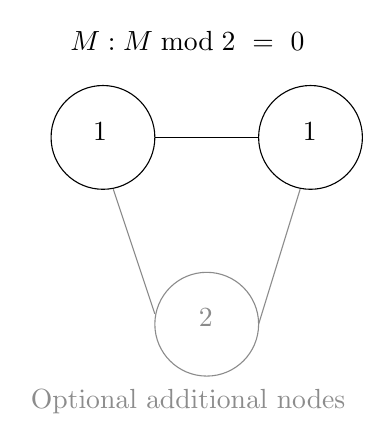
\begin{tikzpicture}[x=0.75pt,y=0.75pt,yscale=-1,xscale=1]
			%uncomment if require: \path (0,224); %set diagram left start at 0, and has height of 224
			
			%Shape: Circle [id:dp8053367545608073] 
			\draw   (360,75) .. controls (360,61.19) and (371.19,50) .. (385,50) .. controls (398.81,50) and (410,61.19) .. (410,75) .. controls (410,88.81) and (398.81,100) .. (385,100) .. controls (371.19,100) and (360,88.81) .. (360,75) -- cycle ;
			%Shape: Circle [id:dp5139832099367154] 
			\draw   (260,75) .. controls (260,61.19) and (271.19,50) .. (285,50) .. controls (298.81,50) and (310,61.19) .. (310,75) .. controls (310,88.81) and (298.81,100) .. (285,100) .. controls (271.19,100) and (260,88.81) .. (260,75) -- cycle ;
			%Straight Lines [id:da34739028917979153] 
			\draw    (310,75) -- (360,75) ;
			%Shape: Circle [id:dp7166484753359771] 
			\draw  [color={rgb, 255:red, 139; green, 139; blue, 139 }  ,draw opacity=1 ] (310,165) .. controls (310,151.19) and (321.19,140) .. (335,140) .. controls (348.81,140) and (360,151.19) .. (360,165) .. controls (360,178.81) and (348.81,190) .. (335,190) .. controls (321.19,190) and (310,178.81) .. (310,165) -- cycle ;
			%Straight Lines [id:da740820997595583] 
			\draw [color={rgb, 255:red, 139; green, 139; blue, 139 }  ,draw opacity=1 ]   (290,100) -- (310,160) ;
			%Straight Lines [id:da5098257307652958] 
			\draw [color={rgb, 255:red, 139; green, 139; blue, 139 }  ,draw opacity=1 ]   (380,100) -- (371.33,128.18) -- (360,165) ;
			
			% Text Node
			\draw (268,22.4) node [anchor=north west][inner sep=0.75pt]    {$M:M\bmod 2\ =\ 0$};
			% Text Node
			\draw (279,66.4) node [anchor=north west][inner sep=0.75pt]    {$1$};
			% Text Node
			\draw (380,66.4) node [anchor=north west][inner sep=0.75pt]    {$1$};
			% Text Node
			\draw (330,156.4) node [anchor=north west][inner sep=0.75pt]  [color={rgb, 255:red, 139; green, 139; blue, 139 }  ,opacity=1 ]  {$2$};
			% Text Node
			\draw (249,195) node [anchor=north west][inner sep=0.75pt]   [align=left] {\textcolor[rgb]{0.55,0.55,0.55}{Optional additional nodes}};
			
			
		\end{tikzpicture}
	}%
	\caption{The base topology from which \textit{Partnerlink} must operate.}
	\label{fig3}
\end{figure}

Each node tracks an additional set of variables. We maintain a set of \textit{locks} against nodes for which operations are still in progress, to protect the system against overlapping requests regarding the same partner. We also maintain an \textit{anticipated} partner count \(M_c\), tracking what our partner count will become if all ongoing non-\textit{panic} operations resolve successfully. Making decisions against this value rather than our actual partner count ensures we do not accidentally request partners above our hard limit \(M\).

\textit{Partnerlink} operations can be split into three categories:
\begin{itemize}
	\item \textit{Initiation}, allowing a healthy node to create new connections with known nodes.
	\item \textit{Panic}, allowing an unhealthy node to recover back to \(M\) connections.
	\item \textit{Leaving}, allowing the overlay to adapt under nominal churn.
	\item \textit{Switching}, incorporating the \textit{DONet} switching mechanism to converge on stronger partnerships.
\end{itemize}
We now discuss the systems and messages in place to allow for these operations.

\subsubsection{\textit{Partnerlink} Initiation} \label{css:partnerlink:initiation}
A node \(n\) entering the network for the first time awaits the first \textit{SCAMP Inview} message to initialize the \textit{Partnerlink} manager. A list of up to \(M / 2\) candidate partners is requested from the contained node, retrieved at random from its \textit{mCache}. This is necessary as the local node's \textit{mCache} needs time to fill with peers; relying on it for first partners comes with substantial startup delay.

\begin{figure}[!ht]
	\centering
	\resizebox{0.8\textwidth}{!}{%
		\input{split.txt}
	}%
\caption{Process of a joining node splitting a partnership}
\label{split}
\end{figure}


Upon reception at node \textit{n}, these nodes are all locked and sent a \textit{Split} message. This performs the split operation discussed in Section \ref{problems:fcn}, attempting to place the node in-between an existing partnership. The node also initializes \(M_c\) to \(M_r * 2\), where \(M_r\) is the number of nodes received from the initial exchange. Node \(a\) receiving a \textit{Split} message checks that no partnership nor lock is held against \(n\) - if not, the node forwards a \textit{TrySplit} message to a random unlocked partner \(b\), holding locks against it and \(n\). Node \(b\) performs the same checks, additionally requiring that \(a\) is not locked. If the checks pass, it returns a \textit{TrySplitSuccess} message, breaks the connection with its old partner and initiates with the new node. Node \(a\) receiving a \textit{TrySplitSuccess} breaks similarly and unlocks the two nodes, after which the exchange is complete. Upon successful TCP connection, node \(n\) removes its lock on node \(a\). The newly joined node has now gained two links, breaking only one in the process. If all \textit{Split} messages respond successfully, the node will have created exactly \(M\) partnerships.

If node \(b\) fails its checks, it responds a \textit{TrySplitFailure}. If node \(a\) receives a \textit{TrySplitFailure}, fails its own checks or does not know another unlocked partner, a \textit{SplitFailure} is forwarded back to the new node \(n\), reducing \(M_c\) by 2 and unlocking the contacted node. This causes the node to immediately begin panicking.

\subsubsection{\textit{Partnerlink} Panicking} \label{css:partnerlink:panicking}
If a node does not satisfy \(M_c = M\), it is described as \textit{panicking}. A node checks its panic state after each update to \(M_c\), from which we begin to look for alternative ways to create new links in the system.

\begin{itemize}
	\begin{figure}[!ht]
		\centering
		\resizebox{0.8\textwidth}{!}{%
			\input{panic.txt}
		}%
		\caption{Gossiping and recovering a \textit{Panic} message}
		\label{panic}
	\end{figure}
	\item If \(M_c = M - 1\), we cannot fill our empty partners by splitting, as we would breach our limit. We instead gossip a 
	\textit{Panic} message containing our \textit{NodeID} to a random partner, similar to the hypothesized mechanism behind \textit{DONet} partnerships. This message is directed across the network towards panicking nodes with priority, as determined from their gossiped status. Otherwise, the message is directed towards any node that is not the original panicking node or the last hop. As a last resort the message is directed to any available node, or else dropped. If a panicking node receives a \textit{Panic} message it initiates a connection with the contained node and increases its \(M_c\) by 1. The original node receiving this connection does the same, unless it has since stopped panicking, in which case the connection is rejected.
	
	This joins two panicking nodes together directly and grants one new link each. This is mostly effective in very small networks, where nodes impacted by an improper exit are few hops apart. As networks grow and crystallize, the hops between panicking nodes will increase, worsening delay before node recovery. Note that locks do not influence the transmission of this message, as its result on a partner does not influence a node's local link count.
	
	\begin{figure}[!ht]
		\centering
		\resizebox{0.8\textwidth}{!}{%
			\input{panicsplit.txt}
		}%
		\caption{Gossiping and recovering a \textit{PanicSplit} message}
		\label{panic}
	\end{figure}
	
	\item If \(M_c = M - 2\), we fall back to the splitting method. We gossip a \textit{PanicSplit} message containing our \textit{NodeID} to a random partner - mechanically, this operates as a gossiped \textit{Split} request. This message contains a field \textit{LastHopOpinion}, initialized to \textit{CANT\_HELP}. The same direction priorities apply, although now targetting non-panicking nodes and with a restriction on gossiping to locked partners. If a node receives a \textit{PanicSplit} with \textit{LastHopOpinion CANT\_HELP}, the node performs similar checks as in a regular \textit{Split} - that we are not already partnered with nor hold any locks against the contained node. If the checks pass, the message is gossiped to a random unlocked partner with a \textit{LastHopOpinion} \textit{CAN\_HELP}, and the contained node and random partner are locked; else, it is marked \textit{CANT\_HELP}.
	
	If a node receives a \textit{PanicSplit} with \textit{LastHopOpinion CAN\_HELP}, we perform the same checks with an additional requirement that we do not hold a lock against the last hop node. If these checks fail, we throw a \textit{PanicSplitFailed} back to the last hop, who unlocks the contained node and partner. We then repeat our treatment of the message as if \textit{LastHopOpinion} had been \textit{CANT\_HELP}. If these checks pass, we proceed as if from a successful \textit{TrySplit} - a \textit{PanicSplitSuccess} is gossiped back to the last hop, our partnership with it is closed and a new connection is initiated with the contained node. The node receiving the \textit{PanicSplitSuccess} message switches connections similarly. The panicking node receiving the connections increases \(M_c\) by 1 each, unless it has since stopped panicking, in which case it rejects the connection.
	
	This finds two relatively stable nodes within the network and places the panicking node between them. This is mostly effective in large networks, where the gossiped message will quickly find its way to nodes with no knowledge of the sender. In networks with node count \(Nc \leq M + 1\), this message will never resolve. The resolution rate quickly improves from there.
	
	\item If \(0 < M_c \leq M - 3\), we gossip both of the above messages at once.
	
	\item If \(M_c = 0\), we should assume global disturbance amongst our membership peers. The standard \textit{SCAMP} leave procedure should be followed to cleanly disconnect from the membership network in the membership manager, before recontacting the origin to gather a fresh partial view and begin new partnerships from scratch.
\end{itemize}

Each of the above messages contains a time-to-live which is checked at each receiving node. If the timeout expires, the message is dropped. It is the responsibility of each panicking node to resend messages after they time out.

These messages are gossiped to partners, though they could instead be gossiped to members. We suspect that gossiping to partners will guide messages towards nodes with a larger number of partnerships (i.e. those with more stable connections) allowing for more effective recovery, whereas the \textit{mCache} may contain a greater concentration of already-poor connections. We cannot provide any proof of this theory, however, which would prove an interesting topic for future research.

\subsubsection{\textit{Partnerlink} Leaving} \label{css:partnerlink:leaving}
To avoid unneeded panics when disconnecting a node, it is intuitive to pair nodes back together, undoing the splitting we performed to enter. If we perform this at leave time, however, an unclean disconnect will still panic all children, adding \(M\) panicking nodes to the network - a substantial breakdown in overlay structure. Instead, we continually inform nodes of their \textit{associated peer} alongside buffer maps. A clean leave then commands nodes to switch connections to the node they were previously informed of, and nodes detecting a failing node can switch automatically without external assistance. This mechanism allows for overlay repair without any additional control in most cases.

\begin{figure}[!ht]
	\centering
	\resizebox{0.8\textwidth}{!}{%
		\input{leave.txt}
	}%
	\caption{Associating peers and cleanly leaving the network}
	\label{panic}
\end{figure}

Nodes should be associated deterministically - that is, for as long as a node holds the same set of partners, the associated peer for each partner should not change. Given a set of partners \(\{A, B, C, ...\}\), the associated peer for \(A\) is \(B\), and for \(B\) is \(A\). If there is an odd number of partners, the final peer is associated with a null \textit{NodeID}. Peers receiving a buffer map should store the new associated peer corresponding to this partnership, replacing any prior peer. If the partnership fails or times out, the node should first attempt to connect to their associated peer. If this connection fails, the node was associated with null, or no association was ever provided, the node should reduce \(M_c\) by 1, entering a panic state.

A leaving node should send a \textit{Leave} message to each of its peers before ending the connection. Each receiving node should attempt the above procedure regardless of the state of the partnership.

\subsubsection{\textit{Partnerlink} Switching} \label{css:partnerlink:switching}
\textit{coolstreaming-spiked} is designed for compatibility with both \textit{DONet} and \textit{New Coolstreaming} research models. To provide this support, we retain the switching system unique to \textit{DONet}. At a set interval, each node should lock and perform a standard \textit{Switch} procedure on a random node in its \textit{mCache}, without changing \(M_c\). Two additional randomly-chosen associated partners should be locked. If both new links from the \textit{Switch} are successful, these two locked partners should be sent \textit{Leave} messages, so that they reconnect to each other; else, the procedure is abandoned and the two partners are unlocked.

We move on to provide additional insight into the rationale of our design.

\subsubsection{\textit{Partnerlink} Rationale} \label{css:partnerlink:rationale}
The \textit{Split} and \textit{Panic} messages are near-identical to those hypothesized to act within the \textit{DONet} model. Switching could also not be achieved without the inclusion of some similar mechanism. These are essential items for the output required of the partner component.

The \textit{SplitPanic} system primarily acts as a caution against early failure when connecting to initial candidate partners. One downside of the \textit{Split} joining model is the chance of collisions - there is some chance that two candidates contact the same node to perform two splits, which will be rejected under the locking mechanism. Network conditions may also lead to a node being impossible to contact. In either case, it is not unreasonable to expect a number of initially chosen nodes to be unreachable, resulting in a starting \(M_c\) far below \(M\) which would take a long time to recover with the vanilla \textit{Panic} strategy. Whilst performance is not a priority for this model, there is still a minimum bar beyond which research analysis would become clouded by its limitations; such startup delay would pose problematic.

The new \textit{associated peers} approach is ultimately easier to implement than the intuitive leave method associated with a splitting approach. Nodes would have to associate peers and forward them to nodes regardless, with the addition of some special case for nodes leaving without notification. An extra opportunity to apply peer selection algorithms also arises in the choosing pairs of peers to associate for filtering, which researchers may find beneficial. Thus, we consider this approach an improvement over the immediately obvious solution.

Whilst the switching mechanism does provide compatibility, its impact on the model is limited compared to the more integral role the \textit{mCache} takes in replacing partners in \textit{DONet}. Research surrounding peer selection algorithms will therefore appear less impactful under \textit{coolstreaming-spiked} - a more in-depth adaptation may also include the algorithm as part of the \textit{associated peer} system to accentuate its effect.

We move on to the final component of the \textit{coolstreaming-spiked} model - the stream manager.

\subsection{Stream Manager} \label{css:stream}
The stream manager is responsible for converting partnerships to parent-child subscriptions, pushing blocks as necessary, as well as the dissemination of buffer maps.

Each node regularly emits a buffer map to every partner. The syntax of these maps has already been discussed - however, an exception on valid syntax is made for when the node has just entered the network. Once buffer maps have been received from some defined minimum percentage of partners, the node must calculate an ideal starting index based on the known set of latest received blocks. Designating \(H_{{S_i},A}\) as the latest block received block for substream \(S_i\) at node \(A\), the starting index at substream \(i\) is calculated as \[I_{S_i} = \max\{H_{{S_i},q} : q \in partners\} - T_p\] where \(T_p\) is a constant to be introduced later. The ideal placement of the starting playout index is specific to the playout strategy and is an open research question. We expect that buffering systems should place playout at \(\min\{I_{S_i}\}\) and begin playout once a minimum buffer percentage has been filled. Non-buffering approaches are more complicated - playout should be placed such that this buffer percentage will have been filled by the time playout reaches \(\min\{I_{S_i}\}\). The actual ideal calculation for this will likely require additional information to be gossiped between nodes.

A new node has not yet receiving blocks in a given substream \textit{i} should fill its latest block with some exceptional value, either a manually-filtered \textit{null} or a value of -1, unless the node intends to make its first subscription on \textit{i} to that partner. In this case, the latest block on this substream should be listed as \(I_{S_i} - K\) to ensure the partner's stream manager begins transmission from the relevant point. The exceptional value should be filtered to ensure the node is never selected as a parent. 

When a node \(n\) subscribes to a substream through their buffer map, the partnership manager reads and stores the node's latest received block \(R_n\). The manager attends to each subscribing partner with a round-robin strategy. At each step, if the node's buffers contains block with sequence number \(R_n + K\), the manager pushes this block to node \(n\) and updates \(R_n\) accordingly, moving on to the next node. The stream manager should aim to fully saturate a node's outgoing bandwidth - as soon as one block finishes transmission, the next should begin. The stream manager will continue to push all blocks in the substream until the partnership or subscription ends; a parent node will not drop a child under any other circumstance.

For monitoring the service of substream \(j\) to child node \(A\) by parent \(p\), two inequalities are defined:

\begin{flalign}
\max\{|H_{{S_i},A} - H_{{S_j},p}| : i \leq K\} < T_s \\
\max\{|H_{{S_i},q}| : q \in partners\} - H_{{S_j},p} < T_p
\end{flalign}

Inequality (1) caps the distance between the most up-to-date child substream and the target parent substream. If this inequality does not hold, the parent has blocks we need that we are not receiving, implying issues with the connecting link. Inequality (2) caps the distance between the target parent substream and the most up-to-date substream we know across all partners. If this inequality does not hold, the parent is lagging behind the wider swarm, implying connection issues further upstream. At each buffer map and block reception, these inequalities are measured against each substream parent - if either fail, the parent is reselected. The replacement parent is selected randomly from all other partners meeting inequality (2) for the target substream - if no partner meets the inequality, the reselection is cancelled. If any reselection occurs, a new buffer map is immediately sent to the affected parents. A cooldown timer \(T_i\) is set on a per-substream basis to prevent repeated reselection and stabilize the overlay topology. Substreams with active cooldowns will not be checked.

The failure state for the stream manager depends on playout strategy. If buffering is incorporated, the node may fall behind the blocks available in the wider swarm. If playout does not halt, we may still find ourselves in a situation where all partners provide unsatisfactory connections. A number of heuristics could detect either case; a threshold over the filled percentage of the buffer is one simple example. Whatever the method, the stream manager should assume a widespread failure amongst its underlying partners, and initiate the same recovery mechanism as defined in the partnership manager.

\subsection{Comparison of \textit{coolstreaming-spiked} to our implementation} \label{css:comparison}
The implementation tested in Section \ref{results} is not an implementation of \textit{coolstreaming-spiked}; indeed, our results from those experiments have informed our design. They are, however, basically similar. The key differences are:

\begin{itemize}
	\item Our implementation retains the \textit{DONet} version of \textit{SCAMP}, with all its oddities. We do not anticipate this aspect of the system to have any impact on performance, and the component outputs are the same.
	\item Our implementation does not include any locking mechanism - instead, more advanced link counting is used to resolve overlapping message streams without hiding nodes from overlay adjustment. The interactions that arise are nearly impossible to reason and are very likely the reason for the desyncing \(M_c\) and partner counts we note in our results. The locking mechanism is proposed due to our experiences with this other approach. This will have an impact on results, as we expect \textit{coolstreaming-spiked} to perform much more reliably.
	\item Our implementation does not make any use of TCP connections, instead relying on UDP either directly or through \textit{OverSim}'s RPC support. This is related at once to the cut-down paper we worked from, that TCP support in \textit{OverSim} is a somewhat hidden feature, and our own oversight. This negatively impacts our results, as TCP networking is essential in the design of \textit{Coolstreaming}.
	\item Our implementation initiates playout similarly to the described buffering playout strategy, though no other buffering is performed. This strange hybrid approach, whilst not invalid, is unlikely to be seen in a real research model and should ideally instead align with one or the other.
\end{itemize}

The changes we have made to \textit{coolstreaming-spiked} since our implementation aim to resolve the poor performance seen in our results. Although this invalidates our final performance figures, we are confident the changes we have made should improve rather than dampen the model.

\section{Conclusion} \label{conclusion}
In this paper, we discuss several research improvements that could be made on top of the popular P2P streaming network \textit{New Coolstreaming}. The objective of the paper is to implement these improvements in simulation alongside a monolithic \textit{AQCS} solution, taking measurements to quantify their impact on QoE. During implementation, we instead hit upon several key issues within the \textit{New Coolstreaming} protocol for research purposes. The new research-oriented model \textit{coolstreaming-spiked} is produced, with a stronger specification and less variable implementation. As part of this, \textit{Partnerlink} allows nodes within the network to form wide-spanning partnership webs at any scale, without triggering any unnecessary churn or reselection.

\section{Further Research} \label{further}
More investigation on \textit{coolstreaming-spiked} should be performed ahead of its use in research. An updated simulation would prove beneficial to validate the issues identified with our first solution have been rectified by the changes since. Assuming this is successful, it would then be possible to perform the testing initially specified in our methodology. A mathematical model of the network, particularly \textit{Partnerlink}, would also prove fruitful in pinpointing any further technical failures, and could produce optimizations that do not significantly impact our low-complexity requirements. Optimized calculations for the ideal starting playout index and proximity-based inequality 1 would round out the model, suitable for more avenues of research.

\printbibliography
\end{document}
